%
%  PARA TRABALLOS EN GALLEGO USAR (LINEA 12): \usepackage[galician]{babel}
%  PARA TRABALLOS EN CASTELLANO USAR (LINEA 13): \usepackage[spanish]{babel}
%
% Para los acentos usamos codificacion UTF-8 (LINEA 10): \usepackage[utf8]{inputenc} 
% Si se usase la codificacion es_ES.ISO-8859-1 (LINEA 11): \usepackage[latin1]{inputenc}
% La conversion de acentos se hace con: iconv -f UTF-8 -t ISO-8859-1 filename.tex
%
% Como se incluyen figuras eps hay que compilar con: latex traballo , dvipdf traballo
%

\documentclass[12pt,twoside,a4paper]{book}
% pódense engadir todos os packages necesarios
\usepackage[utf8]{inputenc}
% \usepackage[latin1]{inputenc}
\usepackage[galician]{babel}
% \usepackage[spanish]{babel}
\usepackage{wrapfig}
\usepackage{lscape}
\usepackage{rotating}
\usepackage{epstopdf}
\usepackage{listings}
\usepackage{color}
\usepackage{enumitem}
\setlist[description]{style=nextline}
\definecolor{dkgreen}{rgb}{0,0.6,0}
\definecolor{gray}{rgb}{0.5,0.5,0.5}
\definecolor{mauve}{rgb}{0.58,0,0.82}
\lstset{frame=tb,
showspaces=false,breakindent=0pt,
  language=Java,
  aboveskip=3mm,
  belowskip=3mm,
  showstringspaces=false,
  columns=fullflexible,
  basicstyle={\small\ttfamily},
  numbers=none,
  numberstyle=\tiny\color{gray},
  keywordstyle=\color{blue},
  commentstyle=\color{dkgreen},
  stringstyle=\color{mauve},
  breaklines=true,
  breakatwhitespace=false,
  tabsize=3
}
\usepackage{graphicx}
\usepackage[dvips]{epsfig}
\usepackage{amssymb}
\usepackage{eurosym}
\usepackage{float}
\usepackage{latexsym}
\usepackage{a4}
\usepackage{listings}
\usepackage{paralist}
\usepackage{parskip}
\usepackage[shortlabels]{enumitem}
\usepackage{hyperref}
\hypersetup{
    colorlinks,
    citecolor=black,
    filecolor=black,
    linkcolor=black,
    urlcolor=black
}
\setlength{\parindent}{1cm}
% \usepackage{hyperref} % menús no pdf pero non leva ben co package galician

\begin{document}
\pagestyle{empty}
\begin{center}
{\bf\Large UNIVERSIDADE DE SANTIAGO DE COMPOSTELA}

\vspace{0.5cm}

\includegraphics[width=5cm]{figuras/logo_usc.eps}

\vspace{0.5cm}
{\bf\large ESCOLA TÉCNICA SUPERIOR DE ENXEÑARÍA}

\vspace{2cm}
{\bf\LARGE Título do Traballo de Fin de Grao}

\vspace{0.5cm}
{\bf\LARGE Subtítulo do Traballo de Fin de Grao}
\end{center}

\vspace{2cm}
\hspace{4cm}\begin{tabular}{l}
{\it\Large Autor:} \\
{\bf\Large Nome do autor} \\
~ \\
{\it\Large Directores:} \\
{\bf\Large Nome do director} \\
{\bf\Large Nome do codirector} \\
\end{tabular}

\vspace{2cm}
\begin{center}
{\bf\Large Grao en Enxeñaría Informática}

\vspace{0.5cm}
{\bf\large Febreiro 2011}

\vspace{0.5cm}
Traballo de Fin de Grao presentado na Escola Técnica Superior de Enxeñaría da Universidade de Santiago de Compostela para a obtención do Grao en Enxeñaría Informática
\end{center}


\cleardoublepage
\pagestyle{plain}
\pagenumbering{roman}

\includegraphics[width=4cm]{figuras/logo_usc.eps}

\vspace{1cm}
{\bf D. Paulo Félix Lamas}, Profesor do Departamento de Electrónica e Computación da Universidade de Santiago de Compostela, e {\bf D. David González Márquez}, Profesor do Departamento de Electrónica e Computación da Universidade de Santiago de Compostela,

\vspace{1cm}
INFORMAN:

\vspace{1cm}
Que a presente memoria, titulada {\it JDataMotion: unha ferramenta para a visualización dinámica de diagramas de dispersión}, presentada por {\bf D. Pablo Pérez Romaní} para superar os créditos correspondentes ao Traballo de Fin de Grao da titulación de Grao en Enxeñaría Informática, realizouse baixo nosa dirección no Departamento de Electrónica e Computación da Universidade de Santiago de Compostela.

\vspace{1cm}
E para que así conste aos efectos oportunos, expiden o presente informe en Santiago de Compostela, a 08/09/2014:

\vspace{2cm}
\begin{tabular}{lll}
O director, & O codirector, & O alumno, \\
~ \\
~ \\
~ \\
~ \\
~ \\
~ \\
~ \\
Paulo Félix Lamas & David González Márquez & Pablo Pérez Romaní
\end{tabular}

 % paxina de certificación (optativa)
%\cleardoublepage
% \pagestyle{plain}
\chapter*{Agradecementos}
Se se quere pór algún agradecemento, este vai aquí.

 % paxina de agradecementos (optativa) 
% \cleardoublepage
% \pagestyle{plain}
\chapter*{Resumo}
Se se quere pór resumo, este vai aquí.

 % páxina de resumo (optativa) 

\cleardoublepage
\pagestyle{plain}
\tableofcontents
\setcounter{secnumdepth}{5}
\setcounter{tocdepth}{5}
\listoffigures

% Agora incluimos os capítulos. Cambiamos a numeración e as cabeceiras
\cleardoublepage
\pagenumbering{arabic}
\setcounter{page}{1}
\pagestyle{headings}
\chapter{Introdución}
\hyphenation{In-te-re-se}

Na actual sociedade da información, onde a cantidade de datos que se manexan aumenta día a día de xeito exponencial, a minería de datos convértese nunha ferramenta fundamental para poder explotalos de maneira eficaz, co fin último de xerar coñecemento a partir dos mesmos.

Para visualizar estes datos unha das técnicas máis utilizadas son os diagramas de dispersión ou scatterplots. Estes permítennos analizar os datos e atopar con facilidade relacións entre as distintas variables, como a correlación entre elas, a distribución dos puntos no plano, a tendencia dos datos recollidos ou outras características que sería complicado extraer a partir dun simple listado, posiblemente desordenado, de vectores de datos. Non obstante, os diagramas de dispersión restrínxennos a unha perspectiva estática do problema. En moitos deses problemas imos encontrar datos cunha compoñente que os sitúa no tempo. Con este proxecto pretendemos dotar a esta representación da súa perspectiva dinámica, para amosar os datos engadindo outro punto de vista que enriqueza a información extraida.

Deséxase desenvolver unha ferramenta para etiquetar cada punto dun diagrama de dispersión cun valor de significado temporal, de tal xeito que este puidese ser empregado como índice nunha visualización dinámica. Este valor numérico podería referenciar dende o momento de captación da tupla que a contén, ata unha ordenación dos datos atendendo á súa prioridade ou relevancia.

\section{Obxectivos xerais}

A motivación principal deste proxecto é o desenvolvemento dunha ferramenta capaz de visualizar a evolución dun conxunto de datos ao longo dunha magnitude como sería o tempo, ademais de permitir o preprocesado ou manipulación deses datos. Sendo máis específicos, este proxecto busca a realización da análise, deseño e implementación dunha aplicación que consiga: 

\begin{itemize}
\item Facilitarlle ao usuario o procesado de volumes de datos dun tamaño significativo. 
\item Posibilitar o traballo con formatos de arquivo CSV ou ARFF. 
\item Dispor das funcionalidades necesarias para manipular os datos. 
\item Ser capaz de amosar os datos en forma de diagramas de dispersión, con funcións de reprodución básicas. Tamén se debe posibilitar a configuración desta reprodución por parte do usuario. 
\item Aplicar filtros nos datos cos que se traballa, de xeito que se poidan eliminar datos fora dun rango, normalizar os seus valores, etc.
\item Interaccionar co usuario por medio dunha interface simple e amigable.
\item Aplicar nun caso real a ferramenta JDataMotion, para apreciar a súa utilidade.
\item Finalizar o desenvolvemento do proxecto antes do día 13 de Febreiro de 2015.
\end{itemize} 

\section{Relación da documentación}

Esta memoria plasma o proceso de desenvolvemento do proxecto JDataMotion, que persegue os obxectivos citados no apartado anterior.

Os distintos capítulos repártense do modo que segue:

\begin{description}
\item[Capítulo 1. Introdución:] composta por obxectivos xerais, relación da documentación que conforma a memoria, descrición do sistema (métodos, técnicas ou arquitecturas utilizadas e xustificación da súa elección).
\item[Capítulo 2. Planificación e presupostos:] inclúe a estimación dos recursos necesarios para desenvolver este proxecto, xunto co custo (presuposto) e planificación temporal do mesmo, así como a súa división en fases e tarefas.
\item[Capítulo 3. Especificación de requisitos:] inclúe a especificación do sistema, xunto coa información que este debe almacenar e as interfaces con outros sistemas, sexan hardware ou software, e outros requisitos (rendemento, seguridade, etc).
\item[Capítulo 4. Deseño:] rexistra como se realiza o sistema, a división deste en diferentes compoñentes e a comunicación entre eles. Así mesmo, neste apartado determínase o equipamento hardware e software necesario.
\item[Capítulo 5. Exemplos:] Avaliación do grao de cumprimento dos requisitos e tests os verifican.
\item[Capítulo 6. Conclusións e posibles ampliacións.]
\item[Apéndice A. Manuais técnicos:] incluirase toda a información precisa para aquelas persoas que se vaian a encargar do desenvolvemento e/ou modificación do sistema.
\item[Apéndice B. Manuais de usuario:] incluirán toda a información precisa para aquelas persoas que utilicen o sistema: instalación, utilización, configuración, mensaxes de erro, etc.
\item[Apéndice C. Licenza.]
\item[Bibliografía]
\end{description} 
\cleardoublepage
\chapter{Xestión do proxecto}

Neste capítulo comentaremos distintos aspectos relacionados coa planificación de como se vai xestionar este proxecto. Falaremos, por exemplo, da xestión de riscos que conleva o desenvolvemento do software, así coma os métodos de continxencia, prevención ou minimización que seguiremos en caso da incidencia dos mesmos. Cos riscos expostos, abordaremos a metodoloxía de desenvolvemento máis axeitada para o proxecto, de acordo tamén cos obxectivos anteriormente plasmados. Seguiremos coa planificación temporal do proxecto e finalizaremos coa estimación de custo e prazos, así como a xestión da configuración. 

\section{Xestión de riscos}

Na fase de planificación dun proxecto hai que sopesar os distintos riscos aos que estará exposto o seu desenvolvemento, cuantificalos e deseñar estratexias para a súa aparición. Algúns dos riscos nun Traballo de Fin de Grao poden ter graves consecuencias na liña base do proxecto debido á inexperiencia do seu autor, polo que fronte á falta de experiencia hai que esforzarse en mellorar a planificación.

Na análise de riscos valoraremos a probabilidade de aparición e a súa gravidade, para a continuación deseñar unha medida de continxencia, prevención ou minimización. A escala de valoración da probabilidade e da gravidade vai ser:

\begin{itemize}
\item Moi baixa
\item Baixa
\item Media
\item Alta
\item Moi alta
\end{itemize} 

Os riscos considerados son os seguintes:

\begin{itemize}

\item \textbf{Risco 01}
\begin{description}
\item[Nome:] Cambios no alcance durante o desenvolvemento
\item[Descrición:] A lista inicial de requisitos funcionais que se captará nas primeiras reunións cos titores vai sufrir modificacións, incluso co proxecto en etapas avanzadas de desenvolvemento. A súa probabilidade duplícase pola existencia de dous clientes no Traballo de Fin de Grao.
\item[Probabilidade:] Moi alta
\item[Gravidade:] Alta
\item[Medidas de minimización:] Botaremos man da folgura temporal do proxecto (marxe de tempo dispoñible para eventualidades). Os cambios razoaranse cos titores, presentando a lista de requisitos actual e valorando a parte da folgura que consumirían ditos cambios. Tamén se tratará de ter reunións de avaliación cos titores cunha alta frecuencia, para así detectar o antes posible calquera cambio nos requisitos, se ben pode acontecer que se propoñan cambios sobre as primeiras etapas cando o proxecto se atopa en etapas avanzadas.
\end{description}

\item \textbf{Risco 02}
\begin{description}
\item[Nome:] Imprecisión á hora de fixar entregables
\item[Descrición:] A inexperiencia do alumno manifestarase xa nas primeiras entregas programadas. Ao non ter traballado previamente en proxectos desta índole, resultará complicado estimar os prazos de entrega nas primeiras fases do proxecto, tanto por exceso como por defecto.
\item[Probabilidade:] Alta
\item[Gravidade:] Media
\item[Medidas de minimización:] Intentaremos especificar entregas dun contido menor e máis frecuentes, sobre todo nas primeiras fases, para que sexa máis doado comezar a estimar correctamente os prazos de entrega.
\end{description}

\item \textbf{Risco 03}
\begin{description}
\item[Nome:] Imposibilidade de reunirse cun dos titores
\item[Descrición:] Un dos titores non pode acudir a algunha reunión proposta, nin estará nos seguintes 5 días.
\item[Probabilidade:] Alta
\item[Gravidade:] Baixa
\item[Medidas de minimización:] Desenvolverase a reunión co titor dispoñible, sendo mester informar das conclusións sacadas ao outro titor por medio do correo electrónico en canto remate a reunión.
\end{description}

\item \textbf{Risco 04}
\begin{description}
\item[Nome:] Descoñecemento ou inexperiencia coas solucións
\item[Descrición:] O alumno non coñece as posibilidades que teñen as ferramentas das que dispón (librarías, módulos, solucións, etc.).
\item[Probabilidade:] Alta
\item[Gravidade:] Media
\item[Medidas de prevención:] Adicarase un tempo prudencial, nas primeiras fases, a revisar as APIs e a documentación en xeral das librerías, proxectos de terceiros e demais ferramentas que se van empregar, para ser conscientes de como poden solucionar as nosas necesidades.
\end{description}

\item \textbf{Risco 05}
\begin{description}
\item[Nome:] Imposibilidade de finalizar o proxecto en tempo
\item[Descrición:] A folgura está esgotada, e o cumprimento do prazo de entrega vese ameazado.
\item[Probabilidade:] Media
\item[Gravidade:] Moi alta
\item[Medidas de prevención:] Evitaremos na medida do posible recorrer á folgura, e trataremos de seguir a planificación do xeito máis estrito que podamos.
\item[Medidas de minimización:] Poremos en coñecemento aos titores do estado do proxecto e dos seus prazos, para discutir a modificación ou eliminación dalgúns ítems da especificación.
\end{description}

\item \textbf{Risco 05}
\begin{description}
\item[Nome:] Limitación das librarías gráficas
\item[Descrición:] As APIs e librarías gráficas non dan solución todas as nosas necesidades
\item[Probabilidade:] Media
\item[Gravidade:] Alta
\item[Medidas de prevención:] Estudiar a especificación de cada solución e as funcionalidades que ofrece.
\item[Medidas de minimización:] Implementarase de xeito manual a solución que se necesita, podendo partir ou botar man do código da librería.
\end{description}

\end{itemize}

\section{Metodoloxía de desenvolvemento}

A elección da metodoloxía de traballo é un paso importante na planificación de calquera proxecto, xa que a posteriori influirá en varios aspectos deste: a xestión dos seus riscos, a súa tolerancia a cambios externos, a confianza na súa validez, etc. Hai dous enfoques fundamentais: as metodoloxías estritas e as metodoloxías áxiles. As primeiras esixen unha planificación estrita, practicamente inmutable e necesariamente realista de todo o plan de traballo, e son boas cando o conxunto de requisitos é fixo e moi concreto. As segundas, pola contra, son flexibles e adáptanse ben a cada situación, pois nelas asúmese que se van producir variacións nos requisitos.

Sopesando as circunstancias nas que se desenvolve un Traballo de Fin de Grao, onde a experiencia do alumno é practicamente nula no que respecta á xestión de proxectos, semella que deberíamos adoptar unha metodoloxía de traballo que se adapte ás necesidades de cambios que vaian xurdindo, e que consiga en cada entrega recibir certa retroalimentación por parte dos titores, de forma que tras cada iteración podamos ter a seguridade da correspondencia entre o proxecto e o modelo mental de quen o especificou. É dicir, necesitamos unha metodoloxía áxil.

Dentro do compendio de metodoloxías áxiles existentes, decantarémonos pola metodoloxía Scrum \cite{scrum}, pois enfoca todas as súas avaliacións sobre entregas parciais, pero funcionais, para facilitarlle ao receptor do proxecto a valoración do mesmo. Necesítase, polo tanto, unha gran implicación do cliente no proxecto, algo que se pode conseguir dada a dualidade da titoría (é máis doado que haxa un titor dispoñible para realizar a reunión). Por outra banda, os requisitos que constitúen as distintas entregas deben estar priorizados para que o proxecto poida avanzar cun carácter incremental, e ditas entregas deben resultar usables para o cliente.

Scrum define unha serie de ferramentas e de regras, idóneas para levar a cabo o desenvolvemento de proxectos que buscan unha metodoloxía áxil. Os preceptos básicos desta metodoloxía son:

\begin{itemize}
\item Adoptar unha estratexia de desenvolvemento incremental, no canto da planificación e execución completa do produto (é dicir, no canto dunha metodoloxía estrita).
\item Basear a calidade do resultado máis no coñecemento das persoas que o especificaron ca na calidade dos procesos empregados.
\item Solapamento das fases de desenvolvemento (análise, deseño, implementación e probas) no canto da sucesión secuencial que nos ofrecen metodoloxías como a fervenza.
\end{itemize} 

A metodoloxía Scrum comeza coa adquisición de requisitos en reunión co cliente, da cal se extrae un Backlog, é dicir, unha lista ordenada por prioridade de requisitos funcionais (RFs). Ademais, Scrum define o sprint como unidade elemental de tempo de traballo. Un sprint dura entre 1 e 4 semanas, aínda que nós trataremos de manter a súa duración en 2 ou incluso 1 semanas para maximizar a supervisión e xestionar ben os riscos, sobre todo nas etapas iniciais.

Ao término de cada reunión co cliente, revísase o Backlog e incorpórase un certo número de RFs a un novo sprint, o cal dará comezo en canto remate a reunión. Para o remate dese novo sprint (dentro dunha semana no noso caso) terase programada a seguinte reunión, na que se valorará o sprint finalizado e se accederá ao Backlog para acordar o seguinte sprint, e así sucesivamente. A valoración do sprint en cada reunión realízase presentando a lista de RFs de dito sprint, e demostrando ante o receptor do proxecto que cada un dos ítems ou tarefas do sprint funciona correctamente.

Para regular o desenvolvemento desa metodoloxía pódese botar man de diversas ferramentas, de entre as cales nós escollemos Acunote \cite{acunote} para o noso proxecto. Acunote é unha aplicación web especialmente deseñada para a xestión da metodoloxía Scrum. Ten varios plans de prezos, pero nós empregaremos o gratuíto porque as nosas necesidades restrínxense a un equipo de persoal pequeno (o alumno e os dous titores). Entre as prestacións desta ferramenta, sacarémoslle maior proveito ás seguintes:

\begin{description}
\item[Wiki:] Empregarémola para engadir contido visible ao resto de membros do grupo.
\item[Lista de sprints:] Amosa os sprints en 3 grupos: sprints pasados, sprints presentes e sprints futuros. Ao abrir un sprint visualízanse os ítems ou tarefas (requisitos funcionais no noso caso) que o compoñen. Accederemos a este apartado na maioría dos casos para crear novos sprints.
\item[Sprint actual:] Visualiza os RFs do sprint actual. A medida que se vaian completando requisitos funcionais, accederase a esta lapela para cambiar o estado do requisito en cuestión. Os estados posibles son:
\begin{itemize}
\item Non comezado (por defecto)
\item En progreso
\item Reaberto
\item Bloqueado
\item Completado
\item Verificado
\item Duplicado
\item Non se vai realizar
\end{itemize}
\item[Backlog:] Contén todos os ítems (requisitos funcionais) pendentes de ser asignados a un sprint. Este lista cumprimentarase ao principio, cos requisitos funcionais captados e ordenados por prioridade, e logo accederase a ela á hora de asignar RFs aos novos sprints. Na extracción de RFs débese respectar a orde dos mesmos dentro da lista, collendo sempre un número de ítems determinado da parte superior. Estes ítems desaparecerán do Backlog en canto sexan asignados.
\item[Tarefas:] Mostra todos os ítems especificados, independentemente de que fosen asignados a un sprint ou non.
\end{description} 

\section{Planificación temporal}

A metodoloxía Scrum caracterízase como ben dixemos polo solapamento das fases que nun modelo en fervenza estarían ben separadas. As primeiras semanas de traballo estarán adicadas á análise para a captación inicial de requisitos, pero nas sucesivas iteracións ou sprints poderán realizarse en paralelo análise, deseño, implementación e probas. Esta é unha das licencias que outorga o emprego das metodoloxías áxiles. De todos xeitos, aínda dentro da variabilidade destas metodoloxías, podemos dividir a vida do proxecto en unha serie de fases fundamentais:
\begin{description}
\item[Inicio:] Constitúe o primeiro sprint (Sprint 00) da planificación, e durará dúas semanas. Nesta fase programaranse reunións cos titores para realizar a captación de requisitos funcionais (análise de requisitos), e ordenaranse estes por prioridade, dando lugar ao Backlog. Tamén se definirá a especificación de cada requisito e se deseñarán as probas que os verifiquen.
\item[Desenvolvemento:] Abrangue dende o Sprint 01 ata o Sprint 11, ambos inclusive (20 semanas en total). Nesta fase elaborarase o produto de acordo cos requisitos.
\item[Documentación:] Abrangue 5 semanas de traballo. Nesta fase recompilarase toda a documentación xerada nas fases anteriores, e confeccionarase a memoria e máis a presentación, que constituirán os entregables do Traballo de Fin de Grao.
\end{description}

En total, o proxecto traballarase durante un período de 27 semanas (189 días, algo máis de 6 meses), co cal, para realizar as 401,25 horas de traballo necesarias teremos que levar un ritmo de traballo aproximado de 15,28 horas semanais (unha media de 2 horas e cuarto diarias). Non nos convén asumir un ritmo de traballo maior, pois durante ese período de tempo o alumno deberá repartir a súa axenda entre este proxecto, o resto de materias, as prácticas en empresa, etc.

\section{Xestión da configuración}

Todo proxecto ten elementos de interese para incluír na xestión da configuración. Estes elementos caracterízanse porque son candidatos a sufrir cambios que poden ameazar o correcto desenvolvemento do proxecto. A xestión da configuración trata de manter a integridade do proxecto perante a estes cambios. O noso deber é identificar que obxectos do proxecto (sexan entregables ou resultados parciais do mesmo) merecen a súa inclusión na xestión da configuración, e por outra parte, temos que especificar que ferramentas empregaremos para dar soporte a esta característica.

Para este caso consideraremos ao código fonte do proxecto (e máis das súas probas) e á documentación como elementos de configuración. O código fonte é o sustento do noso proxecto, e os cambios no seu contido veranse directamente reflexados no produto a entregar, polo que é mester incluír este elemento na xestión da configuración. Tamén incluiremos o código fonte das probas porque debemos respectar a integridade entre estas e o propio proxecto. Por outra parte, a documentación sufrirá cambios de xeito paralelo ao código, e evolucionará da man deste ao longo da vida do proxecto (rexistrará a súa especificación de requisitos, o seu deseño, etc.), así que tamén debe ser un elemento a considerar en aras de preservar a integridade do proxecto. En resumo, faremos seguimento de cambios dos tres directorios ('src', 'test' e 'doc'), e para iso botaremos man do software GitHub \cite{github}.

Github é unha plataforma para darlle aloxamento a distintos tipos de proxectos, por medio do sistema de control de versións Git. Para aloxar o noso proxecto crearemos un repositorio local e outro remoto, chamando a ambos 'JDataMotion', e outorgándolle ao remoto permisos de lectura e escritura para o alumno e permisos de lectura (ou de escritura tamén, opcionalmente) para os titores. Deste xeito estes poderán descargar a última versión do proxecto en calquera momento, mentres que o alumno poderá ir subindo as modificacións cos cambios implementados cada certo tempo.

O proxecto conterá moitos máis elementos, pero non podemos consideralos a todos aptos para a xestión de configuración por diversos motivos: as librarías empregadas non cambian (e no caso de querer actualizar algunha, asúmese que non deben xurdir problemas de integridade grazas á compatibilidade entre versións), os arquivos de configuración persoal non deben ser almacenados no repositorio, e os ficheiros de código obxecto e de distribución dependen directamente do código fonte (que xa é un elemento de configuración), pois xéranse como resultado da súa compilación.

\section{Análise de custos}

A estimación dos custos de desenvolvemento do proxecto amósase no Cadro \ref{tab:custosLabel}. Para ela, consideramos a adquisición dun novo equipo informático. As horas de traballo neste caso non van ter un valor económico asociado, como consecuencia de que este proxecto pertenza a un Traballo de Fin de Grao, pois as horas do traballo do alumno correspóndense coas que este debe cumprimentar para a obtención do título. Para o consumo eléctrico tivemos en conta o prezo do kWh en España \cite{preciokWh_espana} e fixemos unha estimación \cite{energyusecalculator} do consumo eléctrico dun equipo informático, que a plena potencia pode traballar a 120 W. Considerando que o desenvolvemento do traballo durará 401,25 horas, necesitaremos 120 W * 401,25 h = 48150 Wh = 48,15 kWh. Ademais, sabemos que o salario medio anual dun desenvolvedor de software en España é de 26740 €/ano. Se un ano ten 249 días laborables, o custo por hora deste traballador sería de (26740 \euro/ano) / (249 días laborables/ano) / (8 horas/día laboral) = 13,4237 \euro/hora. Os custos inclúen o IVE, pero trataremos de diferencialos na seguinte táboa.

% Table generated by Excel2LaTeX from sheet 'Hoja1'
\begin{table}[htbp]
  \centering
    \begin{tabular}{rrrrr}
    \textbf{Activo} & \textbf{Cantidade} & \textbf{C.U. sen IVE} & \textbf{IVE} & \textbf{Custo total} \\
    Ordenador portátil & 1     & 570,00 \euro & 21\%  & 689,70 \euro \\
    Horas de traballo & 401,25 horas & 11,094 \euro/hora & 21\%  & 5386,26 \euro \\
    Consumo eléctrico & 48,15 kWh & 0,0663 \euro/kWh & 21\%  & 3,86 \euro \\
          &       &       & \textbf{Total} & 6079,82 \euro \\
    \end{tabular}%
		\caption{Custos}
  \label{tab:custosLabel}%
\end{table}%

A anterior estimación é válida só en caso de que o produto a desenvolver non teña unha finalidade comercial. No caso de que este se pretenda comercializar, certas ferramentas que imos utilizar poderían esixir o pago dunha licencia específica.
\cleardoublepage
\chapter{Especificación de requisitos}

\section{Requisitos funcionais}

\subsection{RF01}
\subsubsection{Título}
Importar arquivos con datos para o experimento
\subsubsection{Descripción}
A aplicación debe permitir cargar do sistema de arquivos un ficheiro que conteña unha secuencia de datos (nun formato axeitado segundo o RNF02) para ser utilizados no experimento.
\subsubsection{Casos de uso relacionados}
\subsubsection{Importancia}
Esencial

\subsection{RF02}
\subsubsection{Título}
Exportar datos
\subsubsection{Descripción}
A aplicación debe permitir almacear nun arquivo o conxunto de datos do arquivo actual (tendo en conta filtrados, modificacións, datos engadidos ou eliminados...). Os arquivos de saída deben respetar o RNF02.
\subsubsection{Casos de uso relacionados}
\subsubsection{Importancia}
Esencial

\subsection{RF03}
\subsubsection{Título}
Gardar sesión
\subsubsection{Descripción}
A aplicación debe permitir gardar en disco a sesión (ou experimento) actual tal e como está no momento de executar esta acción.
\subsubsection{Casos de uso relacionados}
\subsubsection{Importancia}
Esencial

\subsection{RF04}
\subsubsection{Título}
Abrir sesión
\subsubsection{Descripción}
A aplicación debe permitir restaurar unha sesión (ou experimento) gardada anteriormente, de xeito que se atope exactamente igual ca no momento en que se gardou.
\subsubsection{Casos de uso relacionados}
\subsubsection{Importancia}
Esencial

\subsection{RF05}
\subsubsection{Título}
Representar os datos en forma de táboa
\subsubsection{Descripción}
A aplicación debe ser capaz de amosar os datos segundo unha táboa na que figuren cabeceiras, tipos, valores...
\subsubsection{Casos de uso relacionados}
\subsubsection{Importancia}
Esencial

\subsection{RF06}
\subsubsection{Título}
Insertar datos no experimento actual
\subsubsection{Descripción}
A aplicación debe permitir a inserción dinámica de datos no experimento actual.
\subsubsection{Casos de uso relacionados}
\subsubsection{Importancia}
Esencial

\subsection{RF07}
\subsubsection{Título}
Modificar datos no experimento actual
\subsubsection{Descripción}
A aplicación debe permitir a modificación dinámica de datos no experimento actual.
\subsubsection{Casos de uso relacionados}
\subsubsection{Importancia}
Esencial

\subsection{RF08}
\subsubsection{Título}
Eliminar datos no experimento actual
\subsubsection{Descripción}
A aplicación debe permitir a eliminación dinámica de datos no experimento actual.
\subsubsection{Casos de uso relacionados}
\subsubsection{Importancia}
Esencial

\subsection{RF09}
\subsubsection{Título}
Asignar tipos aos atributos dun arquivo importado
\subsubsection{Descripción}
A aplicación debe permitir especificar os tipos de atributos presentes no arquivo importado. Por exemplo, os datos cuantitativos poderían ser enteiros ou reais, mentras que os cualitativos serían algo distinto (mesmamente strings).
\subsubsection{Casos de uso relacionados}
\subsubsection{Importancia}
Esencial

\subsection{RF10}
\subsubsection{Título}
Sinalar identificación temporal
\subsubsection{Descripción}
A aplicación debe permitir sinalar unha columna que exprese o orde ou a temporalidade dunha tupla, ou ben definir esta columna manualmente.
\subsubsection{Casos de uso relacionados}
\subsubsection{Importancia}
Esencial

\subsection{RF11}
\subsubsection{Título}
Representar graficamente mediante scatterplot
\subsubsection{Descripción}
A aplicación debe ser capaz de representar gráficamente (mediante scatterplots) o conxunto de parámetros de entrada. Concretamente, débense poder representar ata 4 parámetros por cada scatterplot (ordeadas, abscisas, cor e forma dos puntos). A cor e a forma representan valores discretos, pero ademáis a forma pode representar valores continuos no caso dun degradado. Todos os scatterplots estarán englobados dentro do ``menú de visualización'', que cumprirá co RNF06.
\subsubsection{Casos de uso relacionados}
\subsubsection{Importancia}
Esencial

\subsection{RF12}
\subsubsection{Título}
Engadir scatterplots ao menú de visualización
\subsubsection{Descripción}
A aplicación debe permitir engadir dinámicamente novos scatterplots dentro do menú de visualización.
\subsubsection{Casos de uso relacionados}
\subsubsection{Importancia}
Esencial

\subsection{RF13}
\subsubsection{Título}
Eliminar un scatterplot do menú de visualización
\subsubsection{Descripción}
A aplicación debe permitir eliminar un scatterplot do menú de visualización.
\subsubsection{Casos de uso relacionados}
\subsubsection{Importancia}
Esencial

\subsection{RF14}
\subsubsection{Título}
Configurar un scatterplot do menú de visualización
\subsubsection{Descripción}
A aplicación debe permitir especificar para cada scatterplot do menú de visualización a tupla de atributos a comparar. Tamén se debe poder elixir dende o eixo de representación para cada atributo como a cor ou forma dos puntos. Ademáis tense que dispoñer da opción especificar numéricamente a posición x0 e y0 na que comeza a ventá de visualización, e o ancho e alto desta ventá, o cal constitúe implícitamente un xeito de situar a ventá de visualización, de facer zoom sobre ela e no caso da relación ancho/alto, mesmo de establecer escalas distintas para cada eixo. Esto último podería omitirse, en beneficio dun comportamento dinámico e por defecto da ventá de visualización, que se adaptaría para englobar a todos os puntos representados.
\subsubsection{Casos de uso relacionados}
\subsubsection{Importancia}
Esencial

\subsection{RF15}
\subsubsection{Título}
Detallar punto seleccionado dentro do scatterplot
\subsubsection{Descripción}
Cada punto (non difuminado completamente) dos scatterplots pode ser seleccionado para ver nun apartado os seus detalles (todos os seus atributos, marca temporal...).
\subsubsection{Casos de uso relacionados}
\subsubsection{Importancia}
Esencial

\subsection{RF16}
\subsubsection{Título}
Resaltar punto en scatterplots
\subsubsection{Descripción}
Cada punto seleccionalo dentro dun scatterplot resaltarase tanto nel coma en todos os demáis scatterplots (que plasmarán outras proxeccións do mesmo punto).
\subsubsection{Casos de uso relacionados}
\subsubsection{Importancia}
Esencial

\subsection{RF17}
\subsubsection{Título}
Desprazar a ventá de visualización por arrastre de cada scatterplot (reposicionar)
\subsubsection{Descripción}
Para cada scatterplot poderemos usar unha ferramenta ``man'' para desprazar a ventá polo scatterplot.
\subsubsection{Casos de uso relacionados}
\subsubsection{Importancia}
Esencial

\subsection{RF18}
\subsubsection{Título}
Facer zoom in e zoom out en cada scatterplot (escalar)
\subsubsection{Descripción}
Para cada scatterplot poderemos usar unha ferramenta de Zoom in e outra de Zoom out para facer zoom do scatterplot. O zoom aumentará ou diminuirá a razón de X1.2
\subsubsection{Casos de uso relacionados}
\subsubsection{Importancia}
Esencial

\subsection{RF19}
\subsubsection{Título}
Escalar e reposicionar dinámicamente
\subsubsection{Descripción}
Para cada scatterplot poderemos seleccionar que a ventá de visualización que o enfoca se adapte dinámicamente ao conxunto de datos representados (movéndose, afastándose, aproximándose... para englobar todos os datos).
\subsubsection{Casos de uso relacionados}
\subsubsection{Importancia}
Esencial

\subsection{RF20}
\subsubsection{Título}
Reproducir a secuencia de datos (Play)
\subsubsection{Descripción}
A aplicación debe de permitir que a visualización dos scatterplots poida basarse na variable temporal (ou de orde) para reproducir a secuencia de datos, amosando os datos de cada scatterplot baixo unha secuencia de vídeo. Nesta secuencia engadiríase á visualización en cada instante a tupla de atributos asociada a esa marca temporal. 
\subsubsection{Casos de uso relacionados}
\subsubsection{Importancia}
Esencial

\subsection{RF21}
\subsubsection{Título}
Difuminar puntos ao longo da reprodución
\subsubsection{Descripción}
A aplicación debe permitir difuminar os puntos xa representados a través do avance temporal.
\subsubsection{Casos de uso relacionados}
\subsubsection{Importancia}
Esencial

\subsection{RF22}
\subsubsection{Título}
Representar estela
\subsubsection{Descripción}
A aplicación debe de permitir que cada novo punto ploteado se ligue ao último representado no scaterplott por medio dunha liña recta.
\subsubsection{Casos de uso relacionados}
\subsubsection{Importancia}
Esencial

\subsection{RF23}
\subsubsection{Título}
Difuminar estela ao longo da reprodución
\subsubsection{Descripción}
A aplicación debe permitir difuminar as estelas xa representadas a través do avance temporal.
\subsubsection{Casos de uso relacionados}
\subsubsection{Importancia}
Esencial

\subsection{RF24}
\subsubsection{Título}
Configurar a reprodución da secuencia de datos
\subsubsection{Descripción}
A aplicación debe de permitir que a visualización dos scatterplots sexa configurable en canto a tempo transcurrido entre marcas temporais cando estas sexan de orde, que a velocidade do Play sexa x1, x2 ou x4 ou que se reproduza cara adiante ou cara atrás. Ademáis débese poder especificar o número de marcas temporais que durará o difuminado dos puntos que se ploteen, de xeito que durante ese intervalo cada punto se vaia difuminando ata desaparecer. Pode ser  0 para que os puntos non se difuminen. A aplicación tamén debe permitir especificar o número de marcas temporais que durará o difuminado das estelas que se ploteen, de xeito que durante ese intervalo cada estela xa debuxada se vaia difuminando ata desaparecer. Pode ser 0 para que as estelas non se difuminen.
\subsubsection{Casos de uso relacionados}
\subsubsection{Importancia}
Esencial

\subsection{RF25}
\subsubsection{Título}
Rebobinado e avance rápido da reprodución (Rewind, FastForward)
\subsubsection{Descripción}
A aplicación debe permitir avanzar e retroceder a alta velocidade (X8) a reprodución.
\subsubsection{Casos de uso relacionados}
\subsubsection{Importancia}
Esencial

\subsection{RF26}
\subsubsection{Título}
Pausar a reprodución (Pause)
\subsubsection{Descripción}
A aplicación debe permitir parar a reprodución na marca de tempo na que se atope ao executar esta acción, mantendo as visualizacións para ese momento.
\subsubsection{Casos de uso relacionados}
\subsubsection{Importancia}
Esencial

\subsection{RF27}
\subsubsection{Título}
Ir a un determinado instante dentro do intervalo temporal da reprodución (GoTo)
\subsubsection{Descripción}
A aplicación debe permitir situarse directamente sobre un instante de tempo, mantendo a reprodución pausada sobre esa marca temporal, e visualizando os scatterplots tal e como deben estar nese momento.
\subsubsection{Casos de uso relacionados}
\subsubsection{Importancia}
Esencial

\subsection{RF28}
\subsubsection{Título}
Insertar filtros para os datos do experimento
\subsubsection{Descripción}
A aplicación debe permitir engadir unha serie de filtros que se aplicarán de xeito secuencial sobre a secuencia de datos coa que se esté a traballar. Chamarémoslle "secuencia de filtros" a esta secuencia.
\subsubsection{Casos de uso relacionados}
\subsubsection{Importancia}
Esencial

\subsection{RF29}
\subsubsection{Título}
Gardar unha subsecuencia de filtros do experimento
\subsubsection{Descripción}
A aplicación debe permitir gardar unha subsecuencia de filtros dentro dos que se estén aplicando sobre o experimento. Esta subsecuencia pode comprender tanto un só filtro como a secuencia de filtros enteira.
\subsubsection{Casos de uso relacionados}
\subsubsection{Importancia}
Esencial

\subsection{RF30}
\subsubsection{Título}
Cargar unha secuencia de filtros para o experimento
\subsubsection{Descripción}
A aplicación debe permitir cargar do sistema de arquivos unha secuencia de filtros que se engadirá á cabeza da secuencia de filtros (a cal pode estar vacía). Esta secuencia tamén pode estar composta por un só filtro.
\subsubsection{Casos de uso relacionados}
\subsubsection{Importancia}
Esencial

\subsection{RF31}
\subsubsection{Título}
Eliminar un filtro para os datos do experimento
\subsubsection{Descripción}
A aplicación debe permitir eliminar un determinado filtro dentro da secuencia de filtros.
\subsubsection{Casos de uso relacionados}
\subsubsection{Importancia}
Esencial

\subsection{RF32}
\subsubsection{Título}
Configurar filtros para os datos do experimento
\subsubsection{Descripción}
A aplicación debe permitir seleccionar un determinado filtro dentro da secuencia de filtros para modificar a regla de filtrado implícita.
\subsubsection{Casos de uso relacionados}
\subsubsection{Importancia}
Esencial

\subsection{RF33}
\subsubsection{Título}
Mover os filtros dentro da secuencia de filtros
\subsubsection{Descripción}
A aplicación debe permitir desprazar un filtro dentro da secuencia de filtros do experimento, de xeito que o orde de aplicación dos filtros varíe. O desprazamento realizarase insertando o filtro en cuestión nunha nova posición.
\subsubsection{Casos de uso relacionados}
\subsubsection{Importancia}
Esencial

\subsection{RF34}
\subsubsection{Título}
Calcular distancia entre dous puntos do plano
\subsubsection{Descripción}
A aplicación debe permitir o cálculo da distancia entre dous puntos do plano.
\subsubsection{Importancia}
Esencial

\subsection{RF35}
\subsubsection{Título}
Configurar a fórmula para achar distancia entre dous puntos do plano
\subsubsection{Descripción}
A aplicación debe permitir a introdución da fórmula que se desexe para calcular a distancia entre dous puntos
\subsubsection{Casos de uso relacionados}
\subsubsection{Importancia}
Esencial

\subsection{RF36}
\subsubsection{Título}
Configurar o menú de visualización
\subsubsection{Descripción}
A aplicación debe permitir cambiar os parámetros de visualización dos scatterplots que compoñen o menú de visualización, por exemplo, a cor das estelas, do fondo, dos eixos... ou a fonte, tamaño de letra...
\subsubsection{Casos de uso relacionados}
\subsubsection{Importancia}
Optativa

\section{Requisitos de calidade}

\subsection{RC01}
\subsubsection{Título}
Latencia mínima para o procesamento
\subsubsection{Descripción}
A aplicación debe responder nun tempo razoable ás operacións executadas polo usuario, e intentar que esa latencia escale de xeito controlado ao aumentar a talla dos parámetros.
\subsubsection{Casos de uso relacionados}
\subsubsection{Importancia}
Esencial

\section{Requisitos non funcionais}

\subsection{RNF01}
\subsubsection{Título}
Formatos de entrada admitidos ao importar e exportar arquivos
\subsubsection{Descripción}
A aplicación debe estar preparada para importar e exportar arquivos en distintos formatos, como son o CSV e ARFF.
\subsubsection{Casos de uso relacionados}
\subsubsection{Importancia}
Esencial

\subsection{RNF02}
\subsubsection{Título}
Modularidade no deseño dos filtros
\subsubsection{Descripción}
A aplicación debe facilitar unha interface para a inclusión e uso de filtros personalizados (.jar) no proxecto.
\subsubsection{Casos de uso relacionados}
\subsubsection{Importancia}
Esencial

\subsection{RNF03}
\subsubsection{Título}
Relación programa-sesión
\subsubsection{Descripción}
Cada instancia do programa debe traballar cunha única sesión (experimento).
\subsubsection{Casos de uso relacionados}
\subsubsection{Importancia}
Esencial

\subsection{RNF04}
\subsubsection{Título}
Representación matricial dos scatterplots
\subsubsection{Descripción}
Os scatterplots represéntanse de xeito matricial, facendo que cada parámetro dentro dun eixo sexa enfrentado a cada un dos demáis do outro eixo, e en cada punto desa dupla se sitúe o scatterplot que compara ambos parámetros. Deste xeito, os scatterplots non son acumulables: se temos un que representa X fronte a Y, non podemos engadir outro que represente X fronte a Y, pois ocuparían ambos a misma cela dentro da matriz de scatterplots.
\subsubsection{Casos de uso relacionados}
\subsubsection{Importancia}
Esencial

\subsection{RNF05}
\subsubsection{Título}
Interface de fiestra para engadir contido
\subsubsection{Descripción}
Dentro do apartado de detalles que ilustrará a fondo os atributos dun punto seleccionado haberá un espacio asociado a unha interface que poderá ser implementada para engadir calquer contido.
\subsubsection{Casos de uso relacionados}
\subsubsection{Importancia}
Esencial


\cleardoublepage
\chapter{Deseño}

Neste capítulo documentarase o proceso de deseño que se irá formando de xeito incremental nas sucesivas iteracións da metodoloxía Scrum. Comentarase a arquitectura do modelo de datos que vai manexar a aplicación, así como a distribución deses datos na aplicación, o que nos obrigará a falar da interface gráfica de usuario. Despois disto, mergullarémonos no que é o deseño e máis a implementación dos compoñentes da aplicación.

\section{Deseño global}

O proxecto que imos traballar podería terse desenvolvido, atendendo á súa especificación, baixo un único módulo de traballo. É unha aplicación de escritorio, é dicir, non existe a necesidade, por exemplo, de facer un módulo cliente e un módulo servidor, e polo tanto poderíamos crear un único proxecto de nome JDataMotion que contivese toda a lóxica necesaria para ler, interpretar e procesar datos externos, fornecidos polo usuario.

Sen embargo, e a pesar de todo isto, debemos considerar o requisito de deseño RD01, que nos obriga a definir e facilitar ao usuario unha interface de programación, a cal lle permitirá programar e ensamblar os seus propios filtros no proxecto. Ademais da interface, teremos que publicar as clases das que esta depende. Desta forma, decidimos que o máis práctico era crear un segundo proxecto, ao que mencionaremos a partir de aquí como JDataMotion.common.

E seguindo nesta liña, crearase un terceiro módulo que se usará para probar e exemplificar a efectividade da relación entre os outros dous. Este proxecto chamarase JDataMotion.filters.sample e conterá algunhas clases que implementarán a interface de filtro publicada en JDataMotion.common.

O diagrama que ilustra as relacións entre os 3 módulos sería o que se expón na figura \ref{disenhoGlobal}. O módulo (ou subproxecto) JDataMotion.common contén a interface IFilter (ademáis doutras clases das que depende a interface). Tanto o JDataMotion (a aplicación) como o JDataMotion.filters.sample dependen do módulo común, e en concreto o JDataMotion.filters.sample deberá implementar a interface naquelas clases que vaian ser susceptibles de ser importadas en forma de filtro polo JDataMotion.

\begin{figure}
\centering
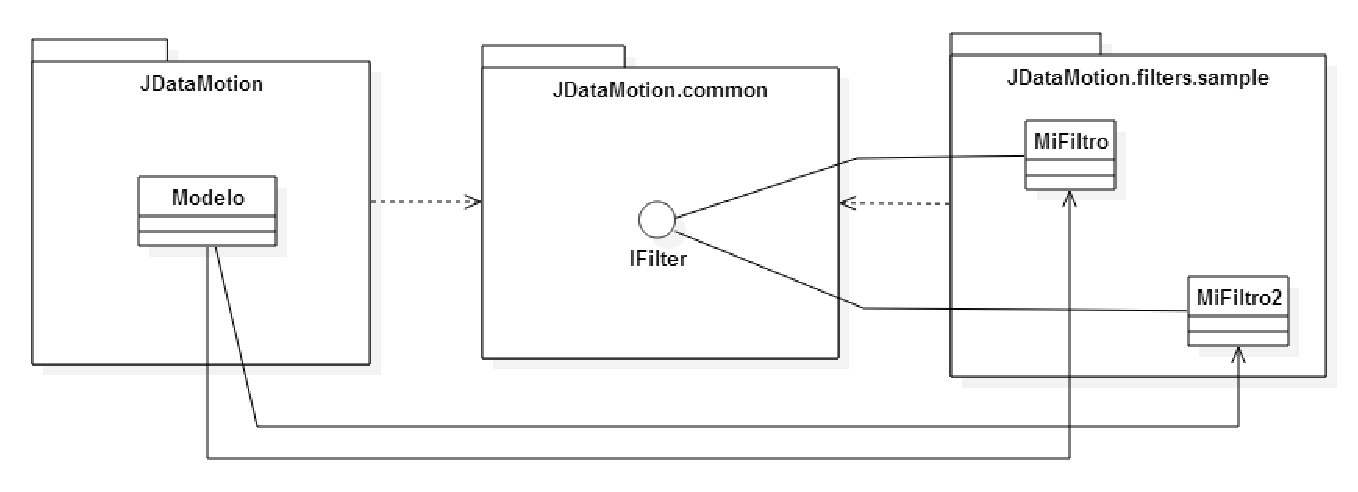
\includegraphics[width=\textwidth,height=\textheight,keepaspectratio]{figuras/disenhoGlobal}
\caption{Deseño global dos 3 módulos que se incluirán dentro do proxecto}
\label{disenhoGlobal}
\end{figure}

A continuación abordaremos o deseño de cada un dos tres módulos implicados neste proxecto.

\section{Deseño de JDataMotion}

Os datos son o punto de partida de todas as funcionalidades deste proxecto. Todo xira arredor do arquivo con información que o usuario importa tras abrir por primeira vez o JDataMotion. O dato debe ser almacenado de xeito adecuado, e accedido só a través dos métodos e clases necesarios, para manter o fluxo de información controlado. A clase que captará, almacenará e distribuirá os datos de cara ás demais clases da aplicación recibirá o nome de Modelo, posto que realmente alberga o modelo da aplicación.

JDataMotion vai ser un programa moi dependente da súa interface de usuario. Os diagramas de dispersión non poden ser visualizados a través dunha simple terminal, e o constante fluxo de datos entre o usuario e o sistema non se pode activar a través dun menú de opcións en termos de usabilidade. Si traballamos co JDataMotion a través dunha interface gráfica multifío como as que Java permite deseñar, a aplicación pode procesar a información ao mesmo tempo que o usuario realiza outras interaccións (ver o modelo, configurar un filtro ou mesmo cancelar a visualización dinámica). Por isto, a clase Vista será un dos artefactos que máis tempo adicaremos a implementar. Vista conterá os ``widgets'' da libraría Swing necesarios para presentar a información ao usuario, e recibir del as novas ordes. Será unha clase complexa e de bastante peso que delegará certas funcións en clases internas ou asociadas.

Só falta unha clase que reciba da Vista as funcionalidades activadas polo usuario e cree un comando que se encargue de realizar o traballo. Esta clase deberá non só disparar o comando, se non que tamén terá que xestionalo, e reaccionar dun xeito específico en caso de que o comando chegue a unha situación de erro. A maioría de comandos influirá directa ou indirectamente sobre o Modelo. A esta clase chamarémoslle Controlador porque a súa responsabilidade será esencialmente esa, a de recibir eventos da Vista e xestionar comandos que actúen de cara ao Modelo. Deste xeito a Vista utilizará a API do Controlador, e quedará exenta de responsabilidade no caso de que se detecten fallas no Modelo.

Acabamos de definir dun xeito explícito cal é o patrón de deseño sobre o que vai xirar toda esta fase do proxecto: o Modelo-Vista-Controlador (MVC). Os patróns de deseño son solucións prácticas a problemas de deseño comúns. En concreto, o Modelo-Vista-Controlador divide o sistema en tres compoñentes coas responsabilidades definidas que xa comentamos anteriormente. A mellor forma de expoñer a aplicación exacta do patrón MVC no noso proxecto é o diagrama da figura \ref{MVC}.

\begin{figure}
\centering
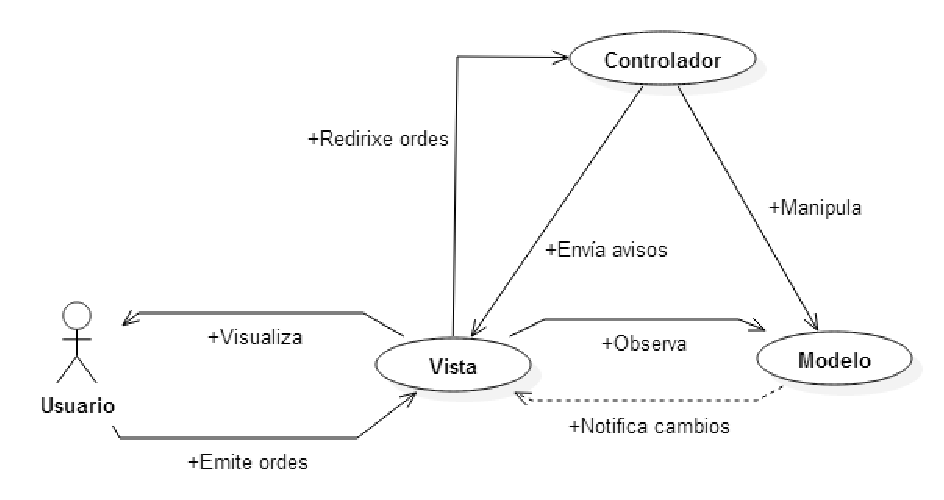
\includegraphics[width=\textwidth,height=\textheight,keepaspectratio]{figuras/MVC}
\caption{Modelo-Vista-Controlador para JDataMotion}
\label{MVC}
\end{figure}

As relacións marcadas cunha liña sólida son asociacións directas (unha clase que actúa de xeito explícito sobre os atributos ou métodos doutra), mentres que a relación marcada cunha liña descontinua representa unha relación indirecta (por exemplo, unha clase que resulta afectada pola actividade doutra). As relacións entre compoñentes detallaranse a continuación.

\begin{itemize}
\item O usuario emite ordes en forma de eventos cara a Vista ao interactuar cos seus botóns e menús.
\item A Vista identifica os eventos que recibe e redirixe cara o Controlador a orde asociada ao evento en cuestión.
\item O Controlador envía un aviso directo á Vista en caso de que a orde que recibe dela levase ao sistema a un estado de erro.
\item O Controlador manipula o Modelo segundo o contido da orde que recibe.
\item O Modelo actúa como entidade observada de cara á Vista. A Vista ten acceso ao Modelo para actualizar a súa aparencia.
\item Do mesmo xeito, que o Modelo sexa observado pola Vista implica que os cambios no modelo serán notificados á Vista, para que esta se actualice no momento do cambio.
\end{itemize} 

Imos documentar máis en profundidade a relación entre a Vista e o Modelo. Comentábamos que a Vista accede ao Modelo para actualizarse cando o desexe, pero ademais o Modelo, cando cambia, notifica á Vista o suceso deste cambio. Temos entón que a Vista actúa como entidade ``observadora'' dun Modelo que é a entidade ``observada''. En esencia, estamos definindo o patrón de deseño Observer.

O patrón de deseño Observer é a mellor resposta que podemos atopar a nivel de deseño para solucionar o problema de manter actualizados ao mesmo nivel o Modelo e a Vista. Se non botásemos man desta solución, teríamos dúas alternativas:

\begin{itemize}
\item Refrescar a vista cada certo intervalo tempo, o cal é ineficiente e seguiría permitindo a posibilidade de que se dese unha incoherencia Vista-Modelo entre refrescos.
\item Permitir ao Modelo que acceda directamente á Vista para invocar un método de actualización, é dicir, asociar directamente a Vista ao Modelo. Isto atenta contra a natureza do Modelo-Vista-Controlador, xa que o Modelo ten que almacenar a información do sistema e abstraerse por completo da Vista ou do módulo que se encargue de representar os seus contidos. Témonos que manter na premisa de que a Vista pode observar ao Modelo e acceder a el para ler datos, pero o Modelo non debe ser consciente da existencia de ningunha Vista.
\end{itemize} 

O patrón Observer pódese aplicar de forma moi sinxela ao noso proxecto. Basta con facer que a Vista implemente a interface \textit{Observer}, de xeito que a obrigue a implementar un método de actualización chamado \textit{update()}, que se disparará cando un obxecto observado cambie o seu estado. Por outra parte, o Modelo só necesita estender a clase \textit{Observable} para ser susceptible de ser observado por un \textit{Observer}. Ao estender esta clase, a Vista xa pode chamar ao método \textit{addObserver(Observer o)} do Modelo, pasándose a ela mesma como parámetro para así incluírse como observadora e ser notificada dos seus cambios.

A asociación dos patróns Modelo-Vista-Controlador e Observer baixo esta forma é bastante común. O libro Pattern-Oriented Software Architecture \cite{pattern-oriented-software-architecture} fai unha boa exposición do que acabamos de mencionar, e aporta o diagrama da figura \ref{MVC-observer} para sintetizar ambos patróns.

\begin{figure}
\centering
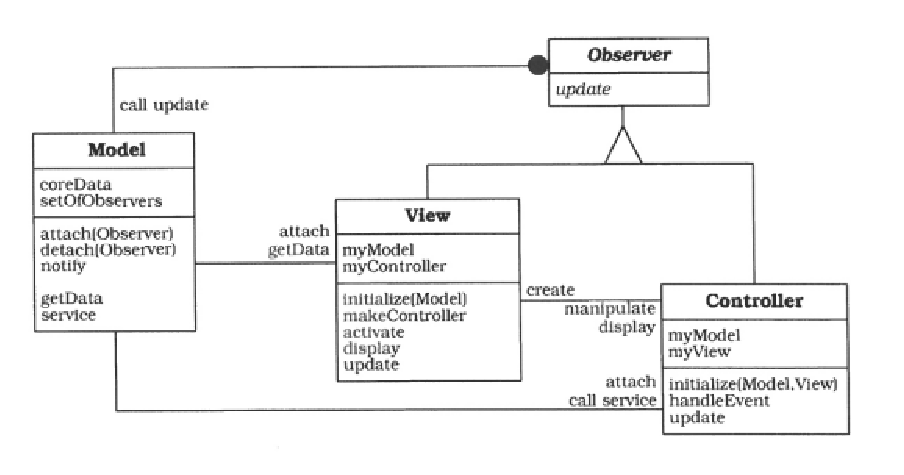
\includegraphics[width=\textwidth,height=\textheight,keepaspectratio]{figuras/MVC-observer}
\caption{Modelo-Vista-Controlador con Observer}
\label{MVC-observer}
\end{figure}

Probablemente a diferencia máis destacable que podemos atopar entre este diagrama e o diagrama que correspondería coa nosa aplicación sería que no noso caso só a Vista implementará a interface \textit{Observer}. O Controlador no noso proxecto non actuará de observador, pois non ten que recibir notificacións ante os cambios do Modelo, xa que de feito el é o responsable directo de todos eses cambios, e non necesita ser notificado de cambios do modelo que non provocase el.

Acabamos de expoñer as 3 clases principais do proxecto e as súas interrelacións, pero debemos ter en conta que cada unha desas clases necesita a axuda doutras que colaboren con ela no obxectivo de cumprir coas súas responsabilidades. O que faremos a continuación será ampliar as 3 entidades básicas do MVC aplicadas ao noso proxecto.

\subsection{Modelo}

O Modelo, como comentábamos, é o responsable de captar e almacenar a información coa que traballamos. A información almacenada clasifícase en 3 conxuntos:

\begin{description}

\item[Instancias:]

Son as tuplas de información coas que se traballa. A estrutura para almacenalas e xestionalas foi reutilizada a partir da API de programación de Weka: a clase Instances. Esta estrutura almacena tanto as propias instancias ou tuplas de información, coma os atributos que levan asociadas. Ademais, contempla toda a información relacionada co atributo: nome, tipo, rango, etc. Esta clase tamén nos facilitará todos os métodos que necesitamos para acceder ou modificar instancias ou atributos. Ademais, a clase Instances de Weka tamén almacena un nome para a relación.

Como veremos, non empregaremos a clase Instances directamente, se non que a estenderemos a través dunha clase á que chamaremos ComparableInstances. A única diferencia entre ambas é que ComparableInstances sobreescribe o método equals(Object o), para determinar que dúas instancias sexan iguais en canto a nome da relación, atributos e tuplas. Isto resultará clave á hora de realizar as probas da aplicación, xa que permitirá verificar que un experimento acada un estado esperado ao aplicarlle unha acción, demostrando a efectividade da mesma.

\item[Filtros:]

O Modelo tamén albergará a secuencia de filtros que utilicemos no noso experimento. Utilizará para isto unha estrutura de tipo lista na que cada novo filtro se engada ao final (se ben é posible cambiar a posición dos filtros e polo tanto a orde da súa aplicación).

Para seren útiles de cara ao Modelo, os filtros deben de conter unha pequena porción de lóxica que a interface IFilter non pode incorporar. Por isto, o Modelo tratará de encapsular cada IFilter co que traballe dentro dun FilterHandler. O FilterHandler só é un manexador da interface que contén, pero con outros campos necesarios como o índice do atributo sobre o que opera o filtro, ou un parámetro de bandeira que indica si o filtro está seleccionado. En canto a métodos, o FilterHandler tamén ofrece ao Modelo un conxunto de procedementos prácticos para traballar co filtro en cuestión.

\item[Outros elementos:]

O Modelo tamén almacena outros datos máis discretos acerca do experimento, como son os índices de atributo temporal e nominal que se empregarán na visualización, a dirección ao ficheiro de orixe e o resumo SHA1 do mesmo (para posibilitar a creación e restauración de sesións).

\end{description}

\begin{figure}
\centering
\includegraphics[width=\textwidth,height=\textheight,keepaspectratio]{figuras/UMLModelo}
\caption{Diagrama de clases do modelo}
\label{UMLModelo}
\end{figure}

A continuación expoñeremos e comentaremos o deseño da sección Modelo. O diagrama de clases preséntase na figura \ref{UMLModelo}. O Modelo debe contar cunha gran batería de métodos útiles para o Controlador. Isto significa que se debe crear un número suficiente de métodos concretos para as necesidades de almacenamento de datos que vaia ter o proxecto, pois as responsabilidades do Controlador non contemplan o traballo directo con unidades de información pesadas como son as ComparableInstances. Isto é, polo xeral será preferible esixirlle ao Modelo unha tupla de información determinada, ca pedirlle todas as ComparableInstances e mesturar dentro do Controlador a xestión de eventos coa procura dunha tupla dentro das instancias totais. En definitiva, en certa medida o Modelo debe ofrecer ao Controlador unha API de programación que atenda ás súas necesidades individuais.

O Modelo, como xa comentáramos anteriormente, estendía a clase Observable (neste caso escolleremos a do paquete java.util). Ademais implementará a interface Sesionizable, que permitirá que os seus campos sexan almacenados nunha sesión para ser recuperados posteriormente. Os dous métodos que deberá implementar serán obterSesion(), que obligará ao Modelo a devolver unha SesionModelo cos datos que desea salvar, e aplicarSesion(Sesion sesion), que tratará de recuperar a sesión a partir da SesionModelo previamente obtida.

Un dos métodos máis destacables do Modelo é notifyChanged(). Este método comproba que o obxecto en cuestión cambiou o seu estado, e en caso afirmativo invoca ao método update(Observable o, Object arg) de todos cantos obxectos estean observando ao Modelo. A comprobación de que o Modelo cambiou realízase cos métodos setChanged() e clearChanged() herdados da clase Observable, que activan ou desactivan unha variable de bandeira. O método setChanged() será chamado polo Modelo cada vez que este acade un novo estado que deba ser notificado (por exemplo, que se engadise unha nova instancia). A continuación, cando o Controlador invoque o notifyChanged() do Modelo comprobarase a bandeira, si esta está activada invocarase ao update(Observable o, Object arg) dos observadores, e a continuación con clearChanged() volverase a desactivar, indicando que non houbo cambios dende a última actualización. O Modelo tamén contén un método reset() que reinicia a súa actividade previa cada vez que comeza un novo experimento.

Outras das clases das que se valerá o Modelo para realizar a súa labor é JarClassLoader. Esta clase estende a MultiClassLoader e utiliza a JarResources para permitir cargar en tempo de execución proxectos .jar xa compilados, posibilitando a importación dinámica de filtros. A clase JarClassLoader será estática e con visibilidade suficiente para permitir que a Vista a use, xa que a vai necesitar para ler directamente dende o directorio onde o Modelo almacena os filtros en .jar que importa.

\subsection{Controlador}

A continuación expoñeremos e comentaremos o deseño da sección Controlador. O diagrama de clases preséntase na figura \ref{UMLcontrolador}. O Controlador é o motor da aplicación, a clase involucrada na maioría das transaccións que afectan ao experimento. A súa tarefa principal é recibir o fluxo de eventos que a Vista notifica, e realizar a operación axeitada en consecuencia. Si a operación require dun procesamento complexo dos datos, o Controlador delegará na lóxica do Modelo para obter o resultado que desexa.

\begin{figure}
\centering
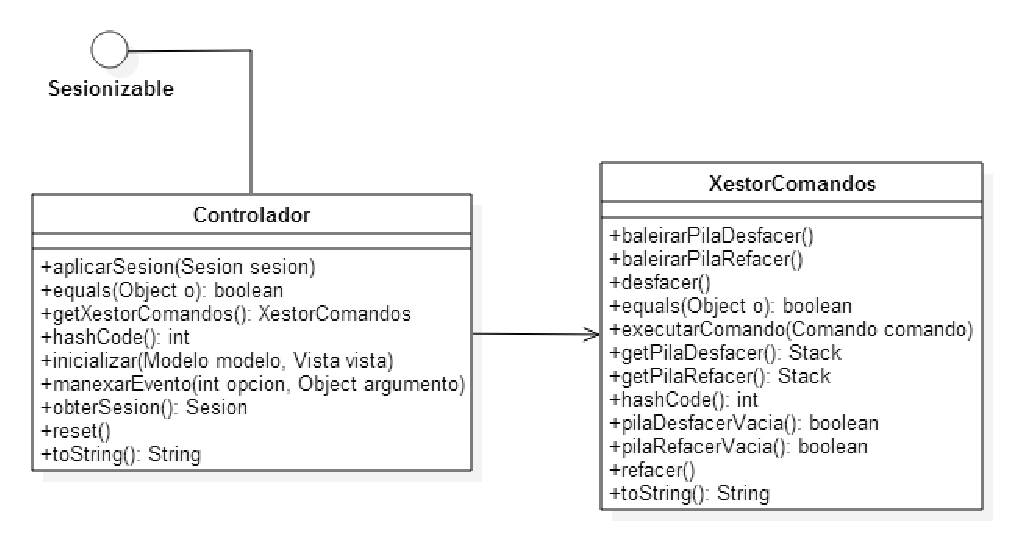
\includegraphics[width=\textwidth,height=\textheight,keepaspectratio]{figuras/UMLcontrolador}
\caption{Diagrama de clases do controlador}
\label{UMLcontrolador}
\end{figure}

O Controlador, do mesmo xeito ca o Modelo, implementa a interface Sesionizable, que permitirá que os seus campos sexan almacenados nunha sesión para ser recuperados posteriormente. Os dous métodos que deberá implementar serán obterSesion(), que obligará ao Controlador a devolver unha SesionControlador cos datos que desea salvar, e aplicarSesion(Sesion sesion), que tratará de recuperar a sesión a partir da SesionControlador previamente obtida.

O Controlador, como motor da aplicación, contén o método inicializar, que recibe unha Vista e un Modelo para comezar a desempeñar as súas funcións. Tamén contén un método reset() que reinicia a súa actividade previa cada vez que comeza un novo experimento.

A pesar de que o Controlador recibe os eventos a través do seu método máis importante: manexarEvento(int opcion, Object argumento). Para procesalos, botará man dunha clase auxiliar chamada XestorComandos, que expoñeremos a continuación. A especificación de que eventos e argumentos pode recibir este método amósase na figura \ref{manexarEvento}. Esta especificación xa figura no código fonte como o JavaDoc do método, de forma que durante a implementación teñamos acceso áxil á especificación deste método, cando estemos configurando dende a Vista as chamadas a este método do Controlador.

\begin{figure}
\centering
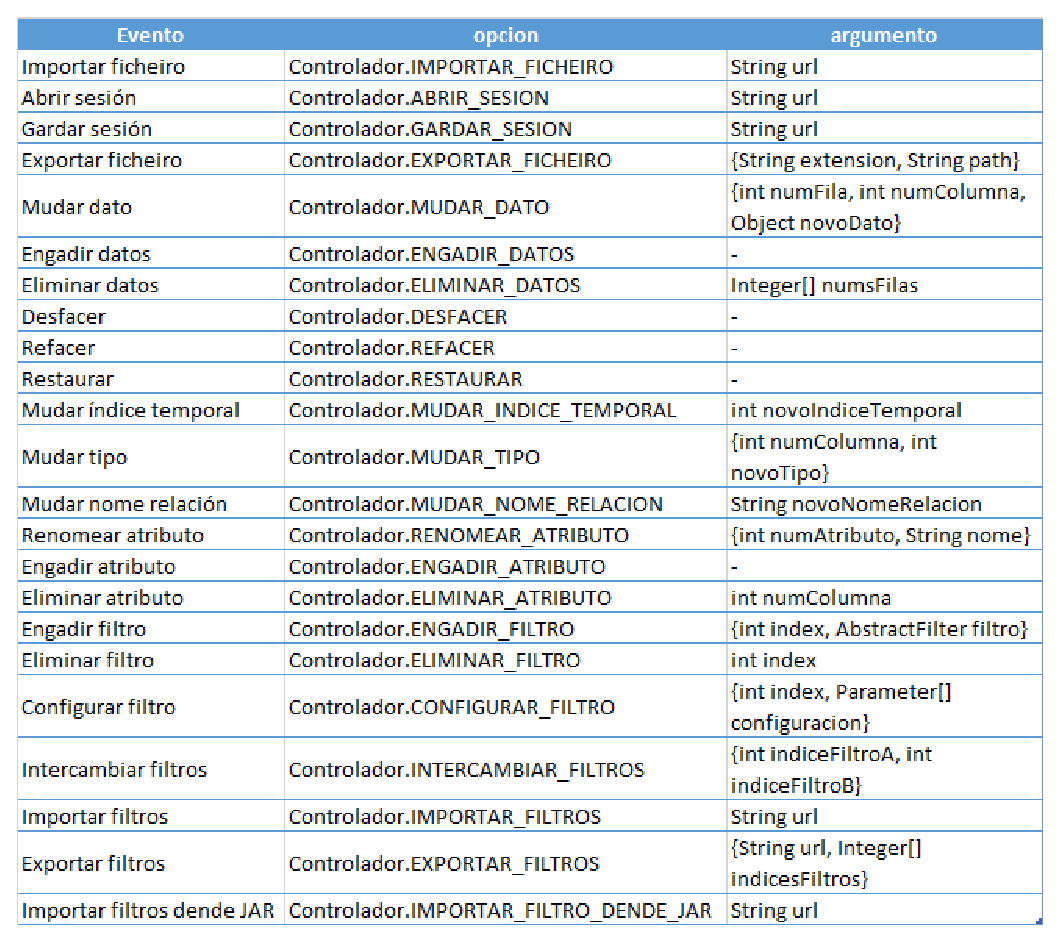
\includegraphics[width=\textwidth,height=\textheight,keepaspectratio]{figuras/manexarEvento}
\caption{Inputs do método manexarEvento}
\label{manexarEvento}
\end{figure}

O parámetro opción é un enteiro que representa ao evento, e todos os valores que pode tomar son constantes declaradas estaticamente na propia clase Controlador. O parámetro argumento debe ser de un tipo ou outro en función da opción escollida. Nos casos nos que na especificación figure unha lista de tipos entre corchetes ({String a, Integer b}), referirase a un array de obxectos ou Object[] (primeiro elemento de tipo String, segundo elemento de tipo Integer).

A clase Controlador recibe eventos a través de manexarEvento, e invoca a un método do XestorComandos para procesalo. Este método non será outro que executarComando(Comando comando). A este método o Controlador debe pasarlle unha instancia do comando que queira procesar, de xeito que a clase Controlador está traducindo eventos que recibe da Vista en comandos que envía ao XestorComandos. Entre as responsabilidades do Controlador tamén está a de recoller as excepcións que poda devolver o XestorComandos, e procesalas adecuadamente (por exemplo ordenándolle á Vista que informe do erro).

Cada vez que se termina de executar un comando, o Controlador solicita ao Modelo a execución de notifyChanged, para que en caso de que este último sufrise modificacións con motivo da execución do comando, a Vista sexa capaz de plasmar a nova información. Xuntando a relación evento-comando coa aplicación do patrón Observer conseguimos que o noso sistema se manteña sempre actualizado ante calquera cambio no Modelo, xa que a causa dos cambios debe pasar polo método manexarEvento do Controlador, e este método sempre remata chamando a notifyChanged. Ambas entidades manteranse sincronizadas sen recorrer a esperas activas ou refrescos innecesarios. Para apreciar mellor as interaccións durante todo este proceso, a figura \ref{DScomandos} contén un diagrama de secuencia que o ilustra.

\begin{figure}
\centering
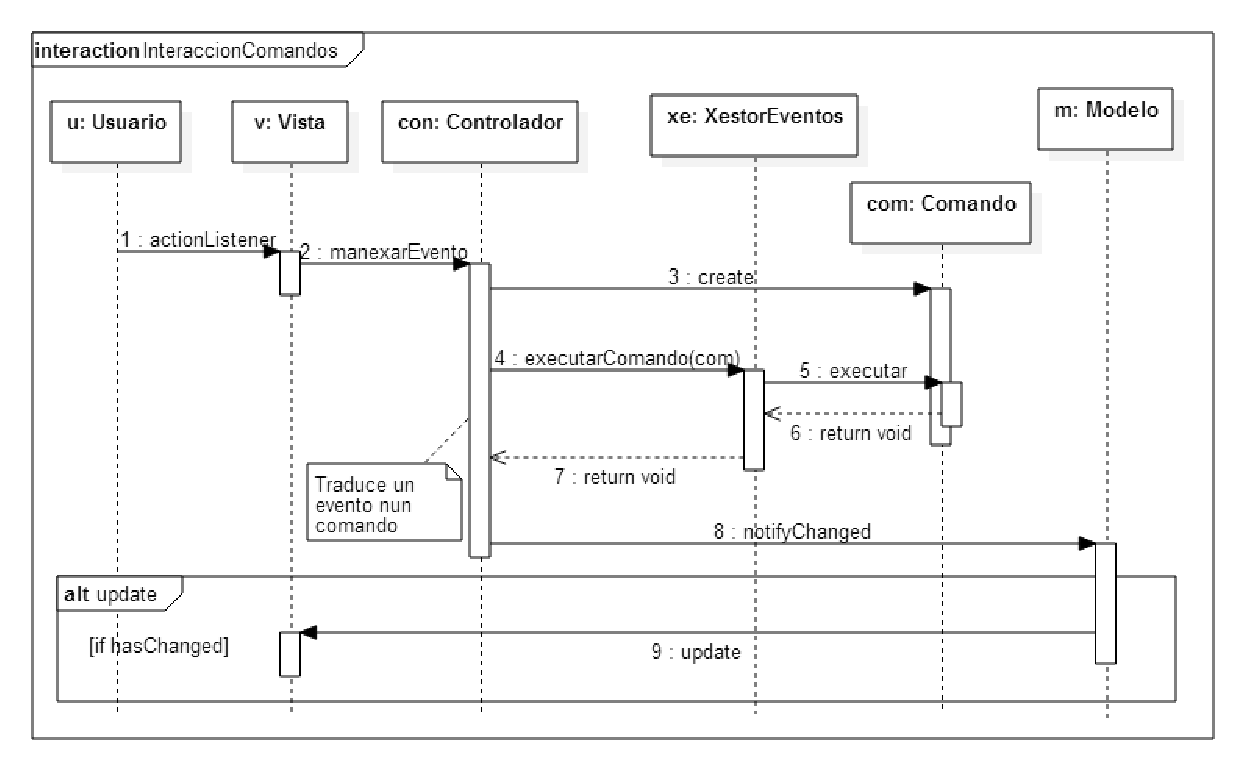
\includegraphics[width=\textwidth,height=\textheight,keepaspectratio]{figuras/DScomandos}
\caption{Diagrama de secuencia evento-notificación}
\label{DScomandos}
\end{figure}

Os comandos que o Controlador emite ao XestorComandos son a forma de manter controladas as transaccións que alteran ao Modelo. Os comandos seguen unha xerarquía que se expón na figura \ref{xerarquiaComandos}.

\begin{figure}
\centering
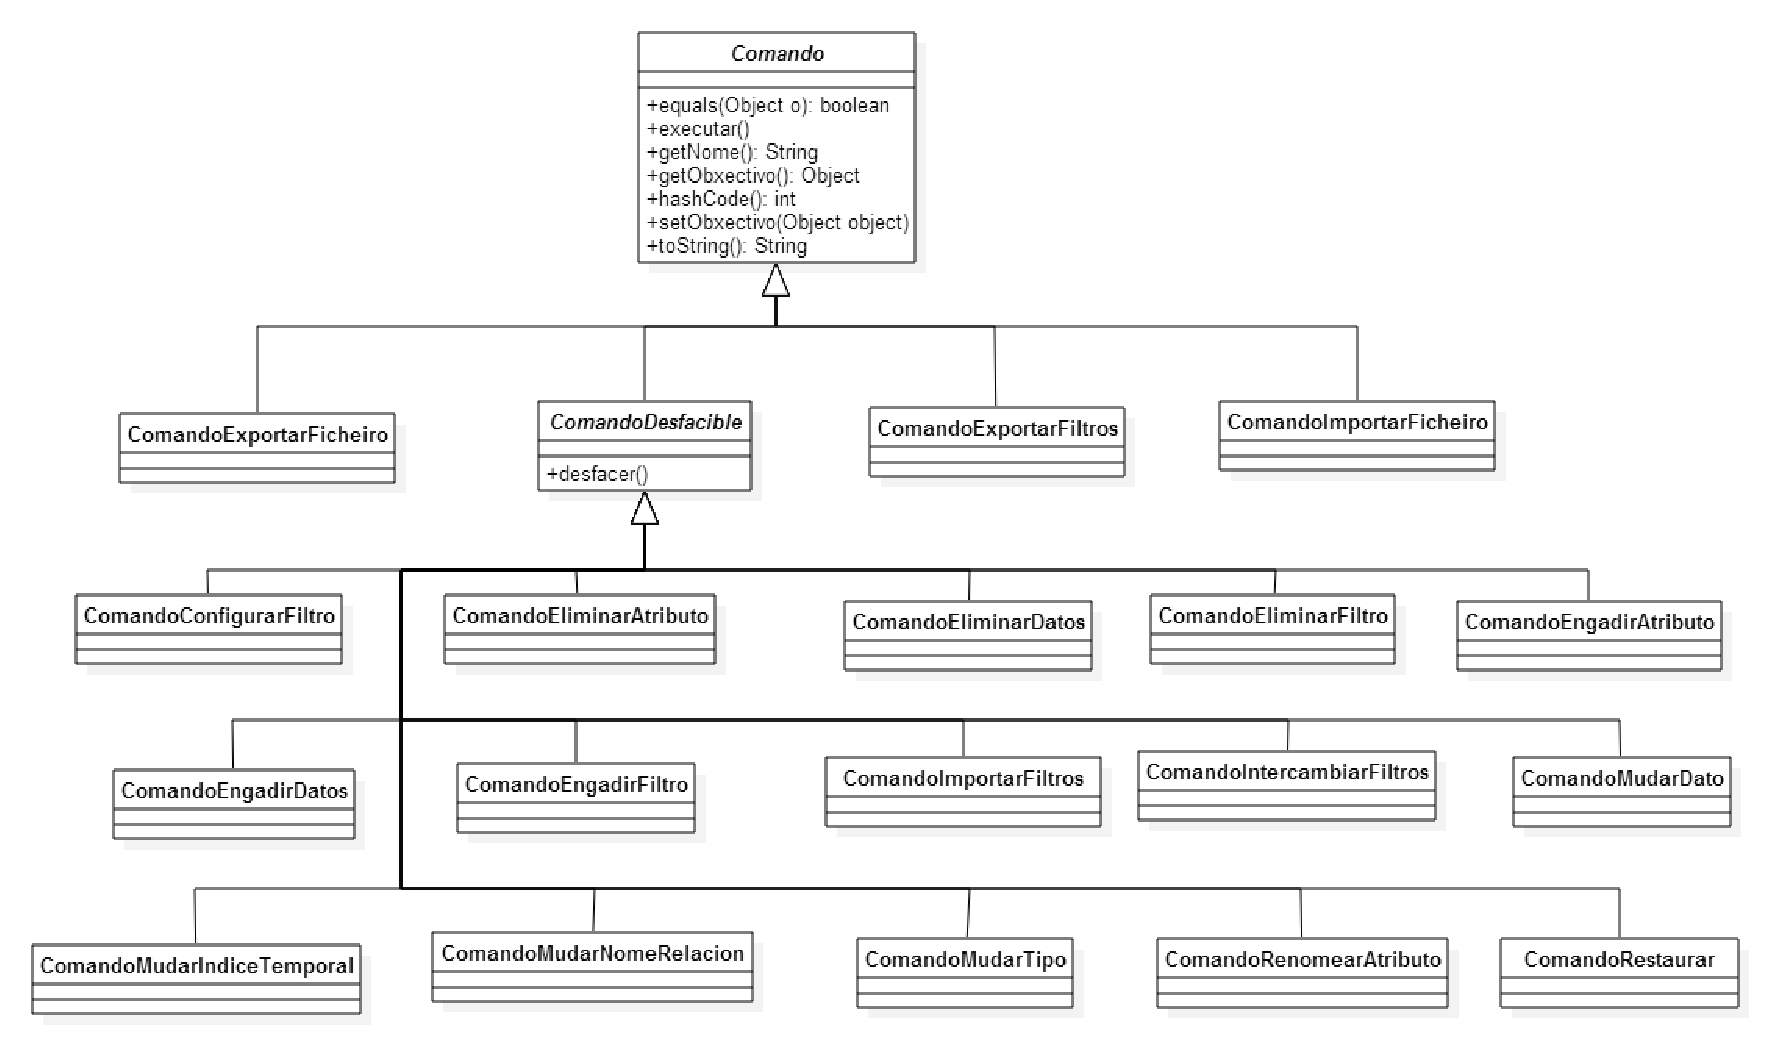
\includegraphics[width=\textwidth,height=\textheight,keepaspectratio]{figuras/xerarquiaComandos}
\caption{Xerarquía de comandos}
\label{xerarquiaComandos}
\end{figure}

Todos os comandos realizan a súa función no método executar(). O construtor da superclase Comando sempre debe recibir un Modelo (ao que tratará co nome de obxectivo). Este obxectivo, que poderemos recuperar por medio de getObxectivo(), é o que se terá que modificar no método executar(). O outro parámetro que debe recibir o construtor de Comando é o nome do comando en cuestión, que poderemos recuperar por medio de getNome().

A maioría de Comandos que o Controlador pode elixir para pasarlle ao XestorComandos son clases que estenderán a superclase ComandoDesfacible. Cando un XestorComandos recibe un Comando que deriva de ComandoDesfacible, almacenarao na pila de desfacer tras a súa correcta execución. Deste xeito, si o Controlador recibe un evento solicitando desfacer o último comando, executará o método desfacer() do XestorComandos directamente. Análogamente poderanse refacer comandos desfeitos. Cabe destacar que os eventos Desfacer e Refacer non xeran comando algún, se non que se tratan chamando ao método desfacer() ou refacer() directamente. O diagrama de secuencia destes dous eventos podémolo observar na figura \ref{xerarquiaComandos}.

\begin{figure}
\centering
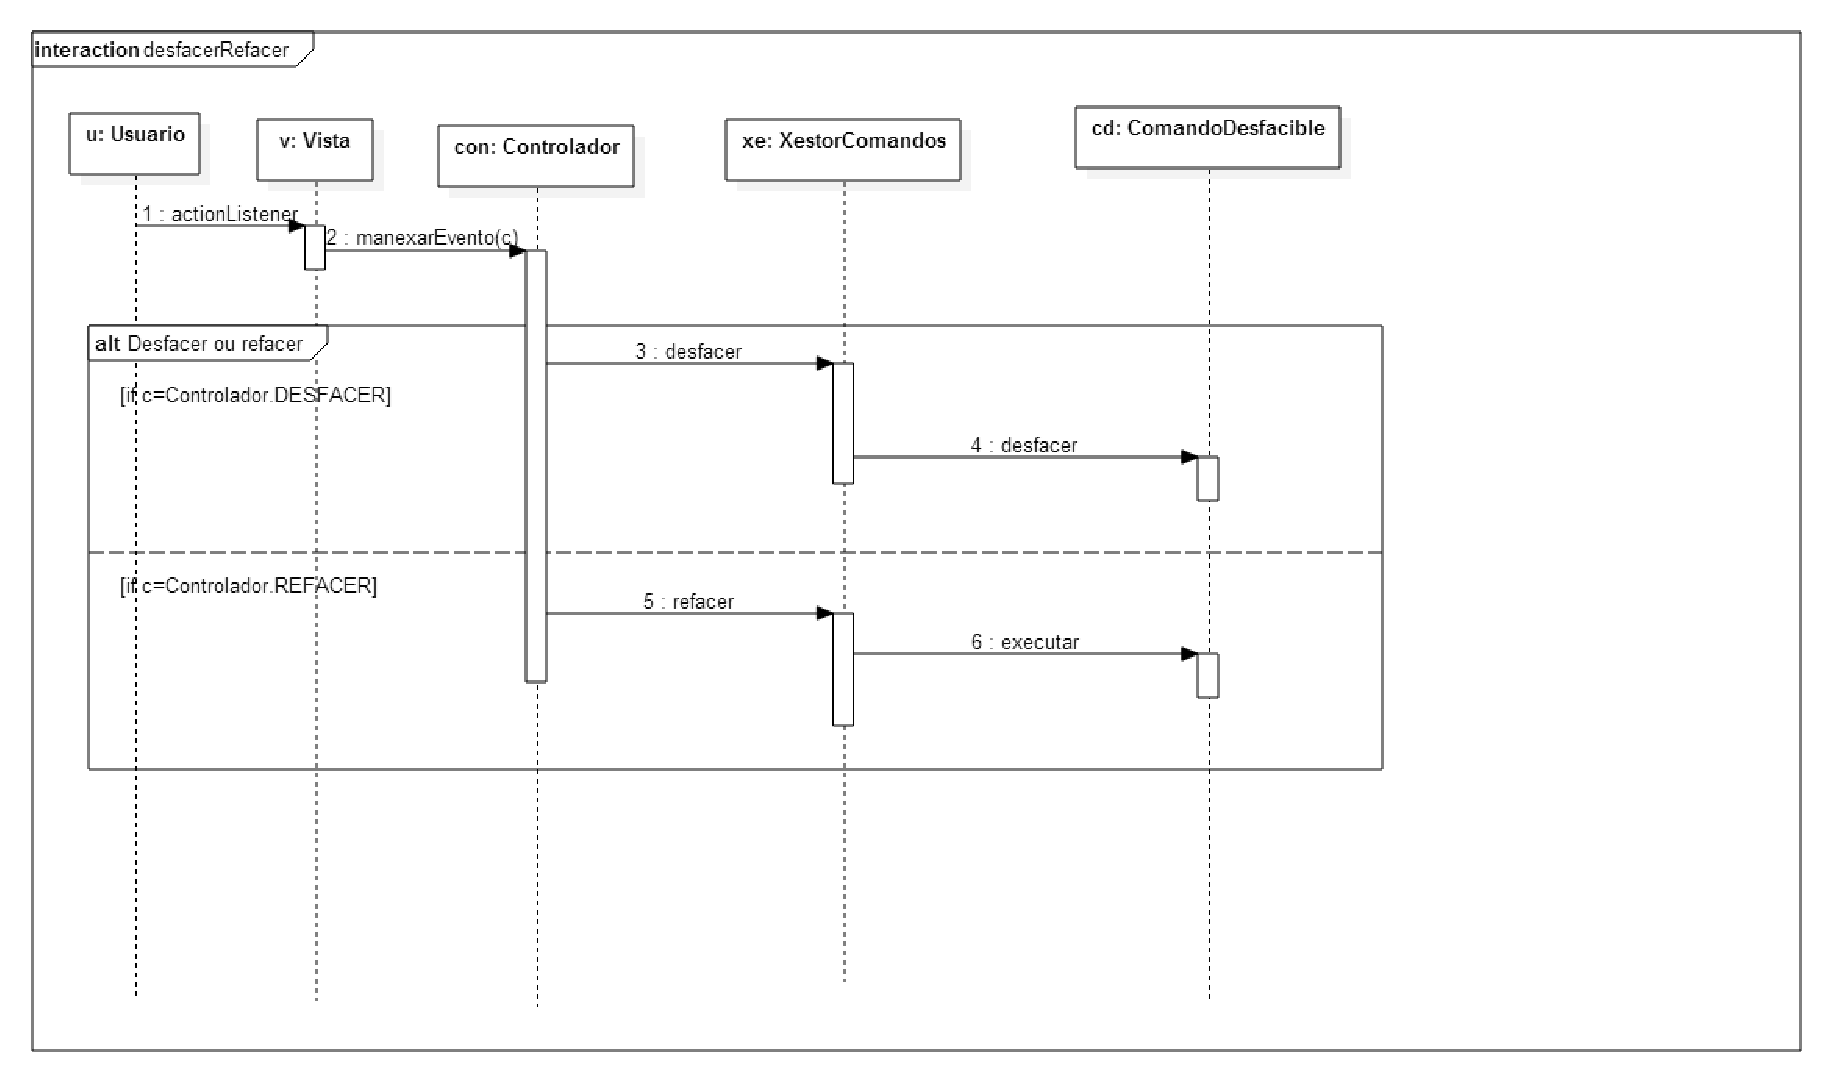
\includegraphics[width=\textwidth,height=\textheight,keepaspectratio]{figuras/desfacerRefacer}
\caption{Diagrama de secuencia dos eventos desfacer e refacer}
\label{desfacerRefacer}
\end{figure}

Do mesmo xeito que se debe implementar o método executar() para todos os comandos atendendo ao seu propósito, no caso dos ComandosDesfacibles tamén debemos implementar o método desfacer(), otorgándolle a este un comportamento que permita inverter os efectos do método executar(). A coherencia entre os procedementos executar() e desfacer() é unha responsabilidade á hora de programar comandos útiles para JDataMotion.

Existe un último grupo de comandos que comentar, e é aquel composto por comandos que aínda que estenden a clase Comando, non estenden a clase ComandoDesfacible. Estes comandos son executados sen posibilidade de entrar ou saír das pilas pilaDesfacer ou pilaRefacer que contén o XestorComandos. Trátase dos seguintes comandos:

\begin{description}

\item[ComandoExportarFicheiro:]

A exportación dun experimento supón a creación dun novo ficheiro no sistema. Esta acción non debe poder desfacerse, xa que atentaría contra a propia finalidade do comando, que é a de salvar permanentemente os datos do experimento no disco duro.

\item[ComandoExportarFiltros:]

Baixo a mesma filosofía anterior, os accesos a disco carecen da necesidade de ser reversibles.

\item[ComandoImportarFicheiro:]

O inicio dun novo experimento reinicia por completo os datos do sistema. Non se deben manter as pilas do XestorComandos dun experimento a outro.

\end{description}

\subsection{Vista}

A continuación expoñeremos e comentaremos o deseño da sección Vista. O diagrama de clases preséntase na figura \ref{UMLvista}. A Vista é

\subsubsection{Deseño da interface gráfica}

Nesta sección configuraremos o deseño da interface gráfica. A Vista é a clase encargada de darlle soporte, delegando certas funcións ou responsabilidades en clases propias asociadas ou internas. Para o deseño da aplicación gráfica teremos en conta as posibilidades da librería gráfica Swing de Java, así como os elementos ou gadgets que a compoñen. 

A utilidade da ferramenta radica no seu uso secuencial: comezamos o noso traballo a partir dun ficheiro (de datos ou de sesión) para revisar os datos e incluso formatealos ou editalos, opcionalmente aplicamos algún filtro global que afecte a todos os campos dunha determinada columna e finalmente visualizamos o resultado. A interface pode colaborar a que este proceso sexa intuitivo, de xeito que dividiremos a interface en tres seccións, ás que se accederá a través de lapelas (o gadget JTabbedPane permitiranos traballar cos 3 contedores de xeito separado). Estas seccións son:

\begin{description}
\item[Modelo:] conterá unha táboa na que cada columna representará un dos atributos, e cada fila unha instancia que pode conter valores para cada un desos atributos. As instancias á sua esquerda unha columna adicional e non editable que indique o índice da instancia. Á dereita da táboa reservaremos un espacio para arroxar información sobre un atributo ao seleccionalo. Por exemplo, ao seleccionar un atributo de tipo numérico (pulsando na cabeceira da columna que o representa) indicarase neste espacio á dereita a media de valores, o máximo, o mínimo, a desviación típica, etc. O mockup desta sección pódese observar na figura \ref{Modelo}.
\begin{figure}
\centering
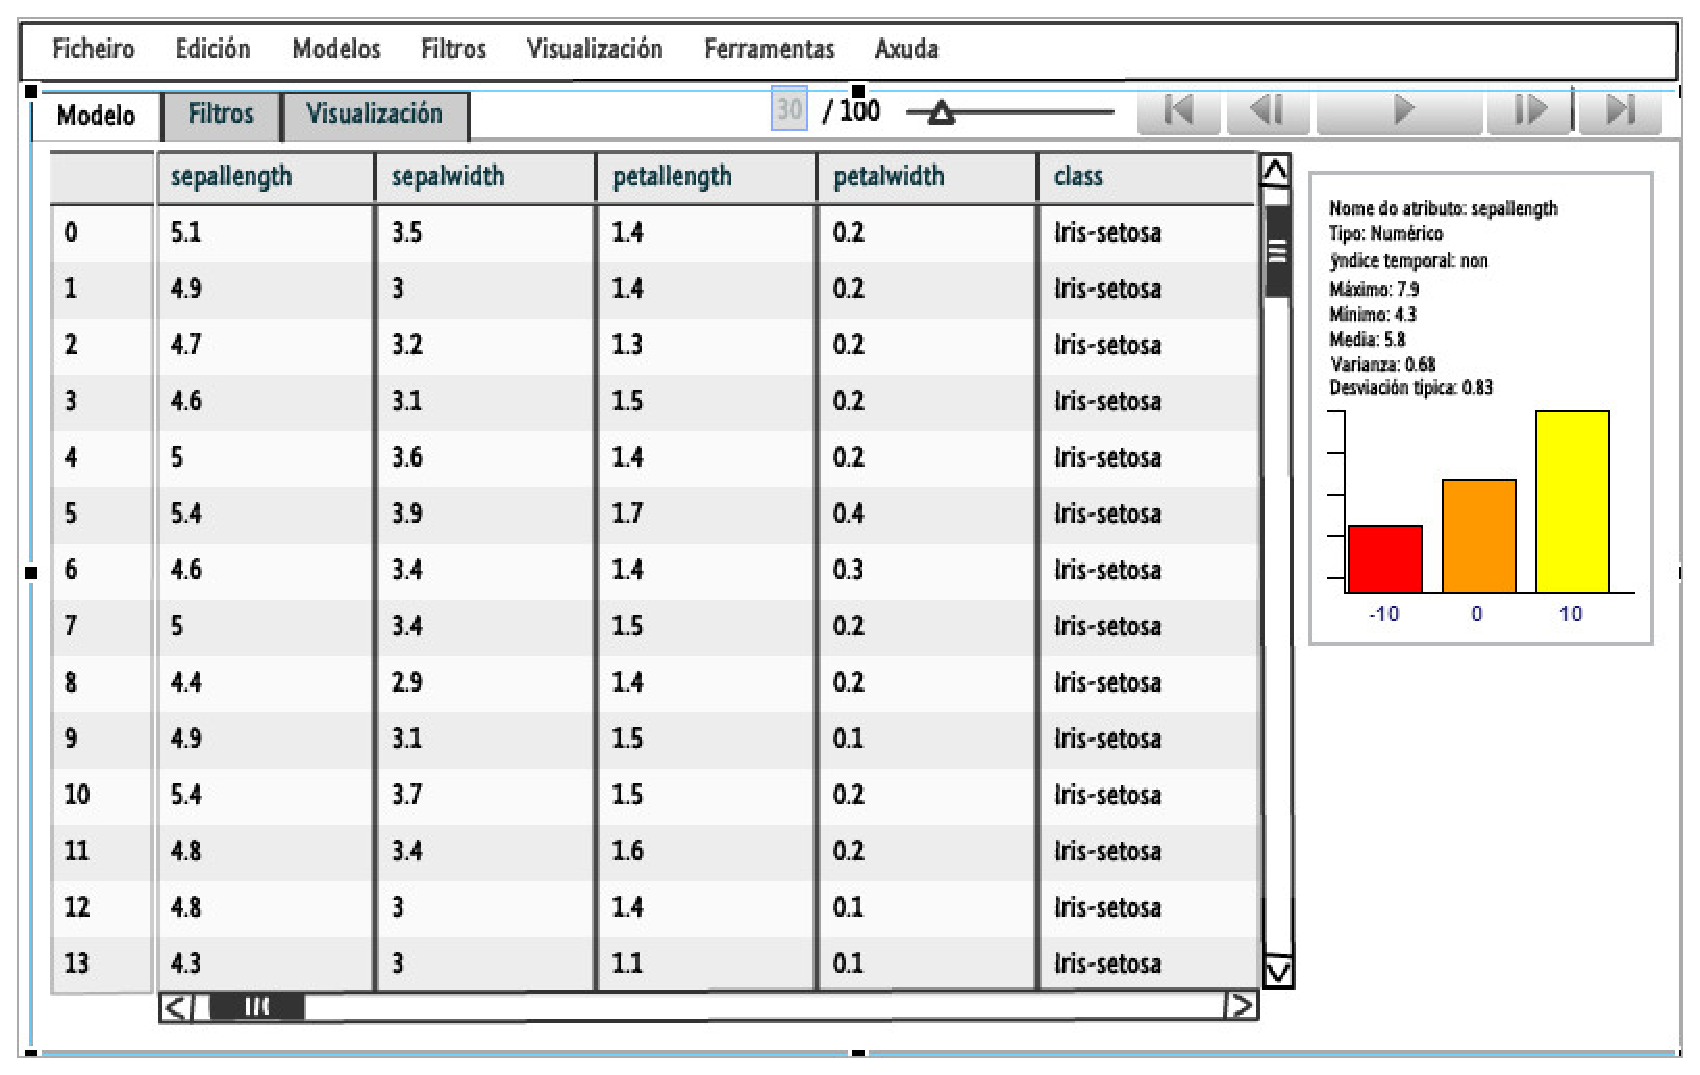
\includegraphics[width=\textwidth,height=\textheight,keepaspectratio]{figuras/Modelo}
\caption{Mockup da sección Modelo}
\label{Modelo}
\end{figure}
\item[Filtros:] conterá unha lista de filtros dispoñibles pegada á borde esquerda, e un botón baixo ela que se active cando haxa un filtro desta lista seleccionado, para engadilo. O resto do contedor ocuparao unha secuencia de iconas en fila, facendo referencia aos distintos filtros que se engadiron e aos modelos parciais que temos antes e despois de cada filtro. O mockup desta sección pódese observar na figura \ref{Filtros}.
\begin{figure}
\centering
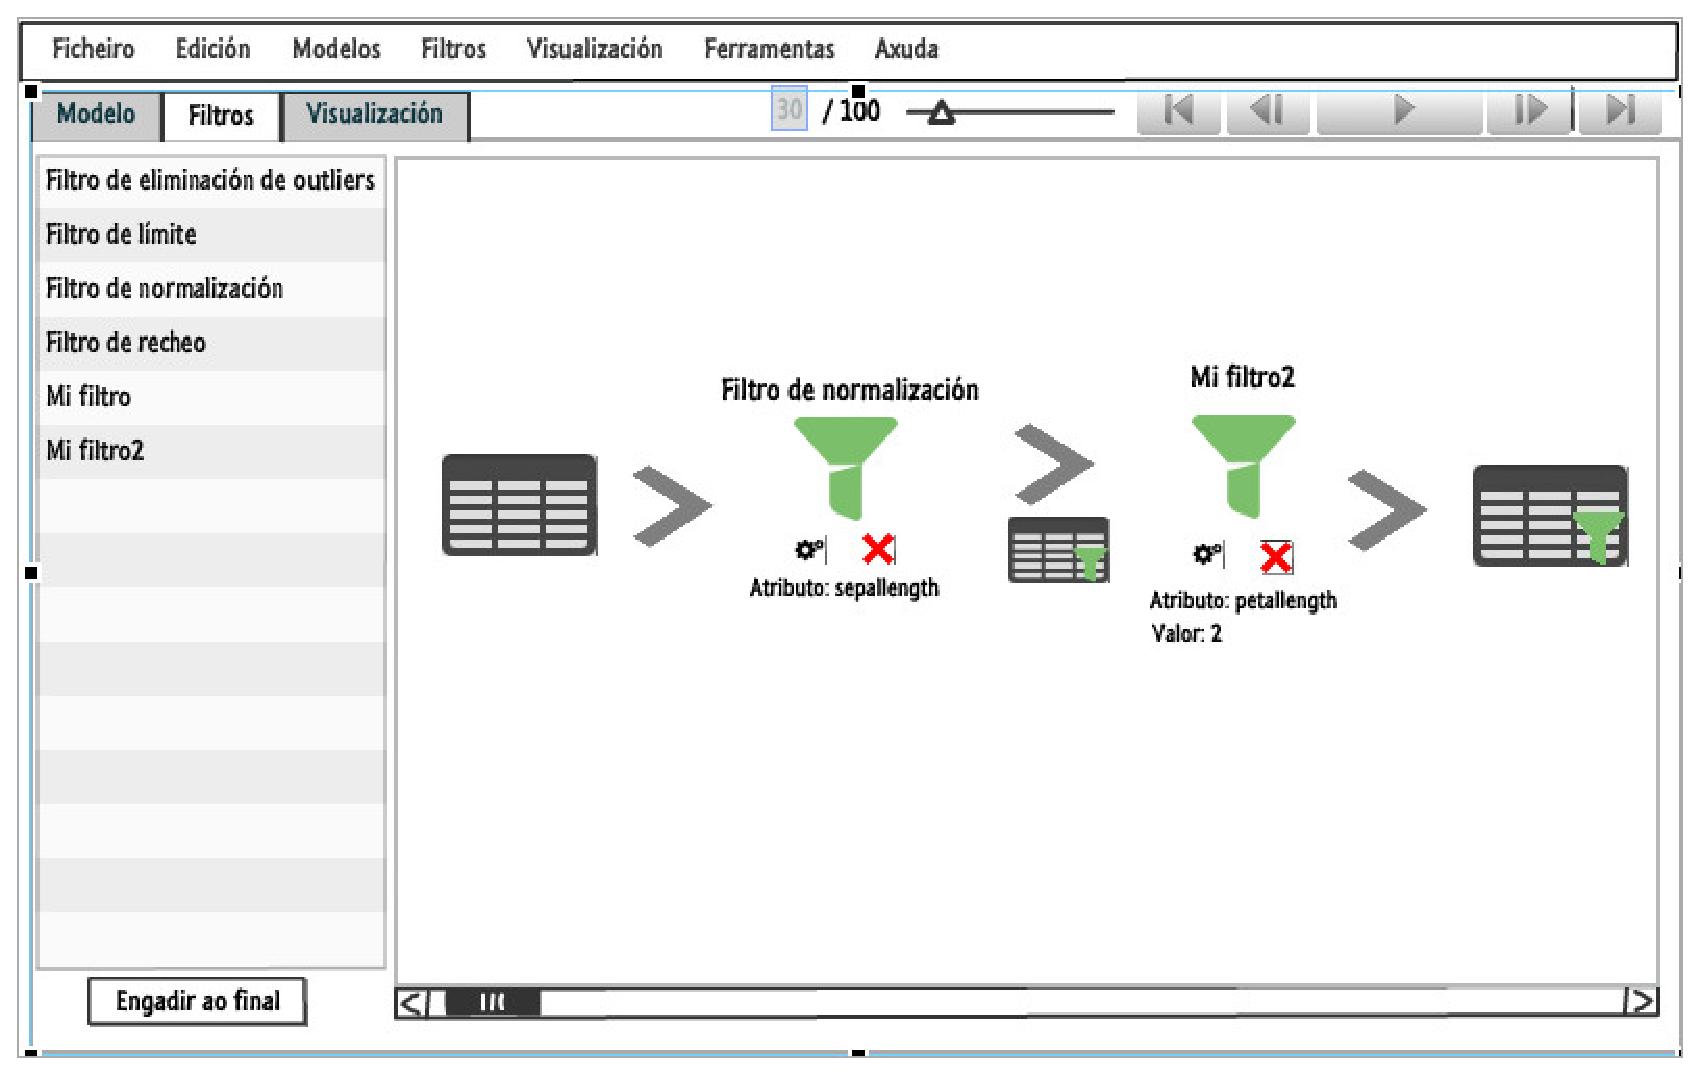
\includegraphics[width=\textwidth,height=\textheight,keepaspectratio]{figuras/Filtros}
\caption{Mockup da sección Filtros}
\label{Filtros}
\end{figure}
\item[Modelo:] a totalidade do espacio para esta sección ocuparao un conxunto de diagramas de dispersión organizados baixo unha matriz, de xeito que en cada fila da matriz os diagramas teñan o mesmo atributo para as ordenadas, e en cada columna da matriz os diagramas teñan o mesmo atributo para as abscisas. Cada diagrama disporá dun botón para ser ampliado nunha ventá aparte. Tamén figurarán dentro desta sección aínda que fora do propio contedor (en liña coas lapelas das seccións) 5 botóns asociados a funcións de reprodución (ir a principio, paso atrás, reproducir/pausar, paso adiante e ir ao final), así como un pivote desprazable ao longo dunha barra (moverase conforme se reproduza o experimento) e un indicador do número de elementos xa visualizados e totais. O mockup desta sección pódese observar na figura \ref{Visualizacion}.
\begin{figure}
\centering
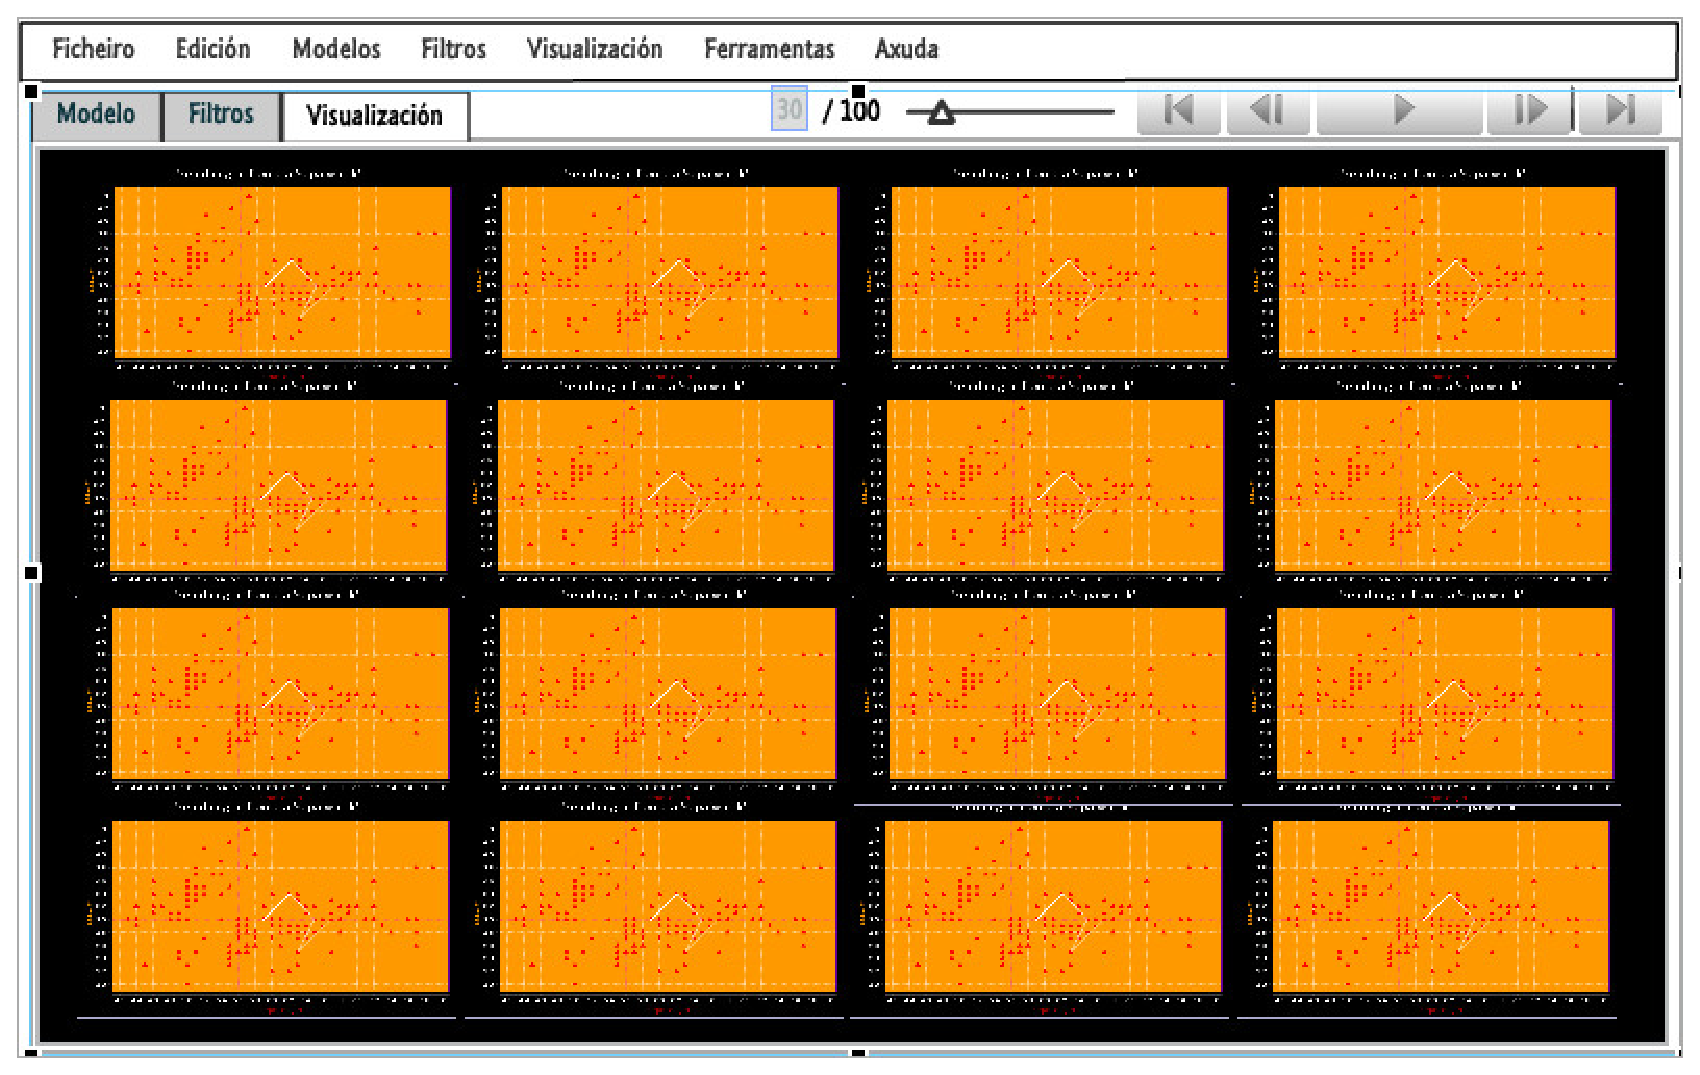
\includegraphics[width=\textwidth,height=\textheight,keepaspectratio]{figuras/Visualizacion}
\caption{Mockup da sección Visualizacion}
\label{Visualizacion}
\end{figure}
\end{description} 

Cada sección foi previamente deseñada a nivel gráfico por medio da ferramenta Lumzy, da cal acabamos de presentar algunhas capturas de pantalla. Para acceder ao mockup e ter unha mínima interacción con el (navegando a través das seccións), podemos utilizar o seguinte enlace (probado a día 10/07/2015):
\\
http://lumzy.com/access/?id=83517845D38CCEEA54A9D6B484A32147

Dada a necesidade do espacio para táboas, listas e sobre todo para a matriz de diagramas de dispersión, adoptouse a medida de desplazar os activadores de case todas as funcionalidades á barra de menús (non operativa no mockup). Prácticamente os únicos botóns que por motivos de usabilidade non podían ser desprazados cara a barra de menús eran os de funcións de reprodución, e de feito tiveron que ir encaixados fóra da propia sección de Visualización sobre a que operan. Entre outros, na barra de menús haberá un título para cada unha das 3 seccións.

Os ítems da barra de menús son os seguintes:

\begin{description}

\item[Ficheiro:] \hfill

\begin{description}

\item[Importar ficheiro:] \hfill \\
Abre unha ventá cun explorador de ficheiros para seleccionar un arquivo en formato .arff ou .csv. A dirección a ese arquivo mándase ao Controlador como argumento, acompañando a un evento de tipo IMPORTAR\_FICHEIRO.

\item[Exportar ficheiro:] \hfill \\
Abre unha ventá cun explorador de ficheiros para seleccionar unha ruta e un nome de arquivo en formato .arff ou .csv. A dirección a ese novo arquivo mándase ao Controlador como argumento, acompañando a un evento de tipo EXPORTAR\_FICHEIRO.

\item[Abrir sesión:] \hfill \\
Abre unha ventá cun explorador de ficheiros para seleccionar un arquivo en formato .jdms. A dirección a ese arquivo mándase ao Controlador como argumento, acompañando a un evento de tipo ABRIR\_SESION.

\item[Gardar sesión:] \hfill \\
Abre unha ventá cun explorador de ficheiros para seleccionar unha ruta e un nome de arquivo en formato .jdms. A dirección a ese novo arquivo mándase ao Controlador como argumento, acompañando a un evento de tipo GARDAR\_SESION.

\item[Restaurar:] \hfill \\
Envía ao Controlador un evento de tipo RESTAURAR.

\item[Pechar:] \hfill \\
Pecha a aplicación JDataMotion.

\end{description}

\item[Edición:] \hfill

\begin{description}

\item[Desfacer:] \hfill \\
Envía ao Controlador un evento de tipo DESFACER.

\item[Rafacer:] \hfill \\
Envía ao Controlador un evento de tipo REFACER.

\end{description}

\item[Modelo:] \hfill

\begin{description}

\item[Engadir instancia:] \hfill \\
Envía ao Controlador un evento de tipo ENGADIR\_DATOS.

\item[Eliminar instancias seleccionadas:] \hfill \\
Envía ao Controlador un evento de tipo ELIMINAR\_DATOS, acompañado dun array de enteiros que contén os índices das filas do Modelo que están seleccionadas.

\item[Engadir atributo:] \hfill \\
Envía ao Controlador un evento de tipo ENGADIR\_ATRIBUTO.

\item[Eliminar atributo:] Envía ao Controlador un evento de tipo ELIMINAR\_ATRIBUTO, acompañado do índice do atributo sobre o que se pulsou.

\item[Renomear atributo:] \hfill \\
Abre un diálogo para introducir o novo nome do atributo pulsado. Envía ao Controlador un evento de tipo RENOMEAR\_ATRIBUTO, acompañado dun array de obxetos co índice do atributo sobre o que se pulsou e o novo nome do atributo.

\item[Mudar nome da relación:] \hfill \\
Abre un diálogo para introducir o novo nome para a relación. Envía ao Controlador un evento de tipo MUDAR\_NOME\_RELACION, acompañado do novo nome.

\item[Amosar todas as columnas:] \hfill \\
Volve a amosar todas as columnas que se ocultaron.

\end{description}

\item[Filtros:] \hfill

\begin{description}

\item[Importar filtros:] \hfill \\
Abre unha ventá cun explorador de ficheiros para seleccionar un arquivo en formato .jdmf. A dirección a ese arquivo mándase ao Controlador como argumento, acompañando a un evento de tipo IMPORTAR\_FILTROS.

\item[Exportar filtros seleccionados:] \hfill \\
Abre unha ventá cun explorador de ficheiros para seleccionar unha ruta e un nome de arquivo en formato .jdmf. Envía ao Controlador un evento de tipo EXPORTAR\_FILTROS, acompañado dun array de obxetos coa dirección do arquivo e un array de enteiros cos índices dos filtros seleccionados.

\item[Importar filtro dende JAR:] \hfill \\
Abre unha ventá cun explorador de ficheiros para seleccionar un arquivo en formato .jar. A dirección a ese arquivo mándase ao Controlador como argumento, acompañando a un evento de tipo IMPORTAR\_FILTRO\_DENDE\_JAR.

\end{description}

\item[Visualización:] \hfill

\begin{description}

\item[Engadir ou eliminar scatterplots:] \hfill \\
Abre unha ventá cunha matriz que enfronta a todos os atributos entre si. Os diagramas de dispersión asociados que se seleccionen ou deseleccionen aparecerán ou desaparecerán da lapela de Visualización.

\item[Establecer atributo nominal representado:] \hfill \\
Abre un diálogo para seleccionar dunha lista despregable de atributos nominais cal se desexa utilizar para diferenciar os puntos nos diagramas de dispersión.

\item[Configurar reprodutor:] \hfill \\
Abre un diálogo que permite modificar a orde da reprodución, o paso e a cor e a lonxitude da estela.

\item[Calcular distancia:] \hfill \\
Abre un diálogo que permite seleccionar dous puntos da lapela de Visualización para calcular a distancia entre eles, segundo unha fórmula editable incluída no diálogo.

\end{description}

\item[Ferramentas:] \hfill

\begin{description}

\item[Idioma:] \hfill

\begin{description}

\item[Galego:] \hfill \\
Cambia o idioma da aplicación a galego (require reiniciar).

\end{description}

\begin{description}

\item[Español:] \hfill \\
Cambia o idioma da aplicación a español (require reiniciar).

\end{description}

\begin{description}

\item[Inglés:] \hfill \\
Cambia o idioma da aplicación a inglés (require reiniciar).

\end{description}

\end{description}

\item[Axuda:] \hfill

\begin{description}

\item[Acerca de:] \hfill \\
Abre un diálogo con información acerca da aplicación e o seu desenvolvemento.

\end{description}

\end{description}

E a continuación comentaremos as funcionalidades que sí se incorporaron na lapela correspondente ao seu ámbito de actuación:

\begin{description}

\item[Modelo:] \hfill

\begin{description}

\item[Botón secundario nun atributo $\rightarrow$ Tipo:] \hfill

\begin{description}

\item[Numérico:] \hfill \\
Envía ao Controlador un evento de tipo MUDAR\_TIPO, acompañado dun array de obxectos co índice do atributo sobre o que se pulsou e a constante Attribute.NUMERIC.

\item[Nominal:] \hfill \\
Envía ao Controlador un evento de tipo MUDAR\_TIPO, acompañado dun array de obxectos co índice do atributo sobre o que se pulsou e a constante Attribute.NOMINAL.

\item[String:] \hfill \\
Envía ao Controlador un evento de tipo MUDAR\_TIPO, acompañado dun array de obxectos co índice do atributo sobre o que se pulsou e a constante Attribute.STRING.

\item[Data:] \hfill \\
Envía ao Controlador un evento de tipo MUDAR\_TIPO, acompañado dun array de obxectos co índice do atributo sobre o que se pulsou e a constante Attribute.DATA.

\end{description}

\item[Botón secundario nun atributo $\rightarrow$ Índice temporal:] \hfill \\
Envía ao Controlador un evento de tipo MUDAR\_INDICE\_TEMPORAL, acompañado do índice do atributo sobre o que se pulsou.

\item[Botón secundario nun atributo $\rightarrow$ Agochar columna:] \hfill \\
Agocha a columna da táboa correspondente ao atributo no que se pulsou.

\item[Botón secundario nun histograma:] \hfill \\
Abre un menú contextual no que se pode almacenar o histograma como unha imaxe, copialo, imprimilo ou cambiarlle o zoom ou a escala.

\item[Selección por arrastre dunha área dentro do diagrama de dispersión:] \hfill \\
Reposiciona e escala o histograma para visualizar a área marcada.

\item[Tecla control + arrastre do diagrama de dispersión:] \hfill \\
Reposiciona o histograma movendo o lenzo na dirección do cursor.

\item[Roda do rato:] \hfill \\
Acerca ou afasta o zoom do histograma.

\end{description}

\item[Filtros:] \hfill

\begin{description}

\item[Botón ``Engadir ao final'':] \hfill \\
Envía ao Controlador un evento de tipo ENGADIR\_FILTRO, acompañado dun array de obxectos co índice que representa a última posición e o filtro que se seleccionou da lista.

\item[Botóns de instancias parciais/finais:] \hfill \\
Abre unha nova ventá co modelo do experimento ao aplicar os filtros ata ese punto da secuencia.

\item[Botón mover filtro á dereita:] \hfill \\
Envía ao Controlador un evento de tipo INTERCAMBIAR\_FILTROS, acompañado dun array de obxectos co índice do filtro sobre o que se pulsou este botón e o índice seguinte.

\item[Botón mover filtro á esquerda:] \hfill \\
Envía ao Controlador un evento de tipo INTERCAMBIAR\_FILTROS, acompañado dun array de obxectos co índice do filtro sobre o que se pulsou este botón e o índice anterior.

\item[Botón configurar filtro:] \hfill \\
Abre un diálogo con campos para cubrir os valores dos parámetros do filtro (o atributo sobre o que se aplica vai incluído). Envía ao Controlador un evento de tipo CONFIGURAR\_FILTRO, acompañado dun array de obxectos co índice do filtro e o array con estes novos valores.

\item[Botón eliminar filtro:] \hfill \\
Envía ao Controlador un evento de tipo ELIMINAR\_FILTRO, acompañado do índice do filtro sobre o que se pulsou este botón.

\end{description}

\item[Visualización:] \hfill

\begin{description}

\item[Botón ``Comezar visualización'':] \hfill \\
Mesmo efecto ca Visualización $\rightarrow$ Engadir ou eliminar scatterplots

\item[Desprazador:] \hfill \\
Permite moverse a distintos puntos da reprodución, chamando ao método goTo() do ManexadorScatterplots e pasándolle a fracción de tempo na que se situou o pivote do desprazador.

\item[Botón ``Ir ao comezo'':] \hfill \\
Leva á reprodución ao instante inicial, chamando ao método goTo() do ManexadorScatterplots e pasándolle o valor 0.0.

\item[Botón ``Paso atrás'':] \hfill \\
Retrocede un paso no reprodución, chamando ao método goToBefore() do ManexadorScatterplots.

\item[Botón ``Reproducir/Pausar'':] \hfill \\
Continúa a reprodución no último punto si esta se atopa parada ou pausada, chamando ao método play() do ManexadorScatterplots. Pausa a reprodución si esta está sucedendo, chamando ao método pause() do ManexadorScatterplots.

\item[Botón ``Paso adiante'':] \hfill \\
Retrocede un paso no reprodución, chamando ao método gotoNext() do ManexadorScatterplots.

\item[Botón ``Ir ao final'':] \hfill \\
Leva á reprodución ao instante inicial, chamando ao método goTo() do ManexadorScatterplots e pasándolle o valor 1.0.

\item[Botón secundario nun diagrama de dispersión:] \hfill \\
Abre un menú contextual no que se pode almacenar a imaxe, copiala, imprimila, cambiarlle o zoom ou automatizar a escala durante a reprodución.

\item[Botón secundario nun diagrama de dispersión $\rightarrow$ Propiedades:] \hfill \\
Este ítem do menú contextual abre unha ventá con opcións de configuración gráfica (colores, fontes, formas, etc.) para aplicar aos diagramas de dispersión desta sección de xeito global. As preferencias establecidas neste menú gardaranse como configuración de usuario.

\item[Selección por arrastre dunha área dentro do diagrama de dispersión:] \hfill \\
Reposiciona e escala o diagrama para visualizar a área marcada.

\item[Tecla control + arrastre do diagrama de dispersión:] \hfill \\
Reposiciona o diagrama movendo o lenzo na dirección do cursor.

\item[Roda do rato:] \hfill \\
Acerca ou afasta o zoom o diagrama de dispersión sobre o que repousa o cursor.

\end{description}

\end{description}

\section{Deseño de JDataMotion.common}

\section{Deseño de JDataMotion.filters.sample}
\cleardoublepage
\chapter{Validación e probas}

Neste capítulo realizaremos o deseño das probas da nosa aplicación. As probas son experimentos cunha especificación determinada. Céntranse en probar un aspecto puntual do sistema, parten dunhas premisas (parámetros, situación, contexto, etc.) definidas a priori, e espérase delas unha resposta consistente. A correspondencia entre o estado ou resposta que se espera da proba e o resultado da súa realización determinan a validez do aspecto que están a probar.

Para probar a nosa aplicación recorreremos a dous métodos, cada un centrarase nun escenario concreto. Por unha parte, a libraría JUnit pon á nosa disposición unha serie de clases, deseñadas para lanzar probas contra pequenos métodos ou bloques de execución. Esta solución será de gran utilidade para validar as funcionalidades que versan sobre o Modelo, xa que o Modelo manipula grandes cantidades de datos que de xeito programático se poden comprobar facilmente.

Os tests en JUnit adoitan finalizar cunha sentencia assetEquals(), que recibe dous obxectos e comproba que sexa iguais para aceptar a proba. En caso contrario devolven un mensaxe de erro e a traza para axudar a solventalo. Para poder asumir que as probas funcionan, necesitamos algo co que comparar os nosos métodos. Nalgúns casos, imos botar man das prestacións da libraría Weka para verificar que o estado final dunha estrutura de datos é o esperado. Deste xeito, poderemos defender que o método funciona apoiándose en que os métodos de Weka co que o validamos xa foron probados previamente.

En base a isto, comezaremos os nosos test creando dous métodos estáticos nunha clase chamada ``ValidFileLoading.java''. Estos métodos son loadARFF(String resourcePath) e loadCSV(String resourcePath). Ambos serán usados de acordo á documentación sobre o seu uso para ler un ficheiro en formato ARFF ou CSV (respectivamente) e extraer del unha instancia de ComparableInstances. Deste xeito xa poderemos asumir como válido que as instancesComparable que devolven son as correctas, as que contén o ficheiro do cal lle pasamos a dirección.

\begin{lstlisting}
public class ValidFileLoading {

    public static ComparableInstances loadARFF(String resourcePath) {
        ComparableInstances comparableInstances = null;
        try {
            ArffLoader loaderARFF = new ArffLoader();
            loaderARFF.setFile(new File(resourcePath));
            comparableInstances = new ComparableInstances(loaderARFF.getDataSet());
        } catch (IOException ex) {
            Logger.getLogger(ValidFileLoading.class.getName()).log(Level.SEVERE, null, ex);
        }
        return comparableInstances;
    }

    public static ComparableInstances loadCSV(String resourcePath) {
        ComparableInstances comparableInstances = null;
        try {
            CSVLoader loaderCSV = new CSVLoader();
            loaderCSV.setSource(new File(resourcePath));
            comparableInstances = new ComparableInstances(loaderCSV.getDataSet());

        } catch (IOException ex) {
            Logger.getLogger(ValidFileLoading.class.getName()).log(Level.SEVERE, null, ex);
        }
        return comparableInstances;
    }

}
\end{lstlisting}

Tamén incluiremos no directorio dos filtros dous ficheiros compatibles con JDataMotion, que empregaremos para realizar as probas: ``213\_N3.csv'' (40 atributos e 3251 instancias) e ``example01.arff'' (1 atributo nominal e 30 numéricos, e 569 instancias)

Sen embargo, JUnit non nos facilita do mesmo xeito a validación de métodos que implican cambios directos na interface de usuario. Probas a nivel gráfico como comprobar que se visualizan correctamente os diagramas de dispersión son menos asequibles realizándoos mediante código ca por simple observación. É por isto que adoptaremos a avaliación heurística para aqueles casos nos que a usabilidade (apariencia intuitiva, sencillez, facilidade de uso, etc.) sexa un importante factor a validar.

A continuación percorreremos de novo todos os requisitos que describimos na análise, para asignarlle un test de proba e executalo mostrando os resultados.

\subsection{Requisitos funcionais}

\subsubsection*{RF01}
\begin{description}
\item[Título] \hfill
Importar arquivos con datos para o experimento
\item[Descrición] \hfill
A aplicación debe permitir cargar do sistema de arquivos un ficheiro que conteña unha secuencia de datos (nun formato axeitado segundo o RNF01) para ser utilizados no experimento.
\item[Importancia] \hfill
Esencial
\item[Tipo de proba] \hfill
Test implementado en JUnit.
\item[Nome do test] \hfill
TestRF01\_1 e TestRF01\_2
\item[Código fonte]
TestRF01\_1:
\begin{lstlisting}
public void test() {
        Modelo modelo = new Modelo();
        Vista vista = new Vista();
        vista.inicializar(modelo, false);
        Controlador.setDebug(true);
        String resource = "example01.arff";
        try {
            String pathEntrada = new URI(getClass().getResource(resource).toString()).getPath();
            ComparableInstances is1 = ValidFileLoading.loadARFF(pathEntrada);
            vista.getControlador().manexarEvento(Controlador.IMPORTAR_FICHEIRO, pathEntrada);
            ComparableInstances is2 = modelo.getComparableInstances();
            assertEquals(is1, is2);
        } catch (URISyntaxException ex) {
            Logger.getLogger(getClass().getName()).log(Level.SEVERE, null, ex);
        }
    }
\end{lstlisting}
TestRF01\_2:
\begin{lstlisting}
public void test() {
        Modelo modelo = new Modelo();
        Vista vista = new Vista();
        vista.inicializar(modelo, false);
        Controlador.setDebug(true);
        String resource = "213_N3.csv";
        try {
            String pathEntrada = new URI(getClass().getResource(resource).toString()).getPath();
            ComparableInstances is1 = ValidFileLoading.loadCSV(pathEntrada);
            vista.getControlador().manexarEvento(Controlador.IMPORTAR_FICHEIRO, pathEntrada);
            ComparableInstances is2 = modelo.getComparableInstances();
            assertEquals(is1, is2);
        } catch (URISyntaxException ex) {
            Logger.getLogger(getClass().getName()).log(Level.SEVERE, null, ex);
        }
    }
\end{lstlisting}
\item[Descrición]
Instáncianse un Modelo e unha vista, inicialízanse utilizando o parámetro visualizacion=false para bloquear a aparición da interface gráfica e actívase a depuración. Importamos o recurso ``example01.arff'' para TestRF01\_1 ou ``213\_N3.csv'' para TestRF01\_2, con axuda dos métodos de Weka nos que imos confiar, e almacenamos as instancias obtidas en ``is1''. A continuación lanzamos ao Controlador un evento de tipo IMPORTAR\_FICHEIRO e almacenamos as instancias do modelo en ``is2''. Por último, metemos ``is1'' e ``is2'' como parámetros do método assertEquals(Object expected, Object actual), e si ambos son iguais o RF01 quedará validado para formatos CSV e ARFF. A sobrescritura do método equals(Object o) dentro de ComparableInstances permitiralle ás instancias desta clase seren pasadas ao assertEquals.
\item[Resultado]
Correcto.
\end{description}

\subsubsection*{RF02}
\begin{description}
\item[Título] \hfill
Exportar datos
\item[Descrición] \hfill
A aplicación debe permitir almacenar nun arquivo o conxunto de datos do experimento actual (tendo en conta filtrados, modificacións, datos engadidos ou eliminados...). Os arquivos de saída deberán respectar o RNF01 en canto a formato de almacenamento.
\item[Importancia] \hfill
Esencial
\item[Tipo de proba] \hfill
Test implementado en JUnit.
\item[Nome do test] \hfill
TestRF02\_1 e TestRF02\_2
\item[Código fonte]
TestRF02\_1:
\begin{lstlisting}
public void test() {
        Modelo modelo = new Modelo();
        Vista vista = new Vista();
        vista.inicializar(modelo, false);
        Controlador.setDebug(true);
        String resource = "example01.arff";
        String tempSaida = "temp01.csv";
        try {
            String pathEntrada = new URI(getClass().getResource(resource).toString()).getPath();
            ComparableInstances is1 = ValidFileLoading.loadARFF(pathEntrada);
            modelo.setComparableInstances(new ComparableInstances(is1));
            String pathSaida = new URI(getClass().getResource(".").toString()).getPath() + tempSaida;
            vista.getControlador().manexarEvento(Controlador.EXPORTAR_FICHEIRO, new Object[]{"csv", pathSaida});
            ComparableInstances is2 = ValidFileLoading.loadCSV(pathSaida);
            is1.setRelationName("");
            is2.setRelationName("");
            assertEquals(is1, is2);
        } catch (URISyntaxException ex) {
            Logger.getLogger(getClass().getName()).log(Level.SEVERE, null, ex);
        }
    } 
\end{lstlisting}
TestRF02\_2:
\begin{lstlisting}
public void test() {
        Modelo modelo = new Modelo();
        Vista vista = new Vista();
        vista.inicializar(modelo, false);
        Controlador.setDebug(true);
        String resource = "213_N3.csv";
        String tempSaida = "temp01.arff";
        try {
            String pathEntrada = new URI(getClass().getResource(resource).toString()).getPath();
            ComparableInstances is1 = ValidFileLoading.loadCSV(pathEntrada);
            modelo.setComparableInstances(new ComparableInstances(is1));
            String pathSaida = new URI(getClass().getResource(".").toString()).getPath() + tempSaida;
            vista.getControlador().manexarEvento(Controlador.EXPORTAR_FICHEIRO, new Object[]{"arff", pathSaida});
            ComparableInstances is2 = ValidFileLoading.loadARFF(pathSaida);
						assertEquals(is1, is2);
        } catch (URISyntaxException ex) {
            Logger.getLogger(getClass().getName()).log(Level.SEVERE, null, ex);
        }
    }
\end{lstlisting}
\item[Descrición]
Instáncianse un Modelo e unha vista, inicialízanse utilizando o parámetro visualizacion=false para bloquear a aparición da interface gráfica e actívase a depuración. Importamos o recurso ``example01.arff'' para TestRF02\_1 ou ``213\_N3.csv'' para TestRF02\_2, con axuda dos métodos de Weka nos que imos confiar, e almacenamos as instancias obtidas en ``is1''. A continuación lanzamos ao Controlador un evento de tipo EXPORTAR\_FICHEIRO, pasándolle a dirección dun arquivo temporal en formato CSV para TestRF02\_1 ou en formato ARFF para TestRF02\_2. Despois disto, utilizamos as clases de importación nas que estamos confiando para obter as instancias dende o arquivo ao que acabamos de exportar e almacenamos o seu contido en ``is2''. Por último, metemos ``is1'' e ``is2'' como parámetros do método assertEquals(Object expected, Object actual), e si ambos son iguais o RF02 quedará validado para formatos CSV e ARFF. A sobrescritura do método equals(Object o) dentro de ComparableInstances permitiralle ás instancias desta clase seren pasadas ao assertEquals. En TestRF02\_1 debemos eliminar os nomes de relación das dúas ComparableInstances para ser xustos, xa que o arquivo ARFF perdeu o seu no proceso de exportación a CSV.
\item[Resultado]
Correcto.
\end{description}

\subsubsection*{RF03}
\begin{description}
\item[Título] \hfill
Gardar sesión
\item[Descrición] \hfill
A aplicación debe permitir gardar en disco a sesión (ou experimento) actual tal e como está no momento de executar esta acción.
\item[Importancia] \hfill
Esencial
\item[Tipo de proba] \hfill
Test implementado en JUnit.
\item[Nome do test] \hfill
TestRF0304
\item[Código fonte]
\begin{lstlisting}
public void test() {
        Modelo modelo = new Modelo();
        Vista vista = new Vista();
        vista.inicializar(modelo, false);
        Controlador.setDebug(true);
        String resource = "example01.arff";
        String archivoSesion = "temp01.jdms";
        try {
            String pathEntrada = new URI(getClass().getResource(resource).toString()).getPath();
            ComparableInstances is1 = ValidFileLoading.loadARFF(pathEntrada);
            modelo.setComparableInstances(new ComparableInstances(is1));
            modelo.setDireccionAoFicheiro(pathEntrada);
            modelo.setHashCodeFicheiro(Modelo.resumirFicheiroSHA1(new File(pathEntrada)));
            String pathSaida = new URI(getClass().getResource(".").toString()).getPath() + archivoSesion;
            /* se modificamos un dato manualmente, a sesion non o rexistra
             e ao restaurar a sesion o arquivo segue sendo igual ao inicial */
            modelo.getComparableInstances().instance(5).setValue(5, 666);
            /* se lanzamos un comando, a sesión rexistrao e entonces a proba fallaria
             porque se volveria a executar o comando ao restaurar a sesion, e xa non seria igual ao inicial */
            //vista.getControlador().manexarEvento(Controlador.MUDAR_DATO, new Object[]{5, 5, 666});
            vista.getControlador().manexarEvento(Controlador.GARDAR_SESION, pathSaida);
            vista.getControlador().manexarEvento(Controlador.ABRIR_SESION, pathSaida);
            ComparableInstances is2 = modelo.getComparableInstances();
            assertEquals(is1, is2);
        } catch (Exception ex) {
            Logger.getLogger(TestRF0304.class.getName()).log(Level.SEVERE, null, ex);
        }
    }
\end{lstlisting}
\item[Descrición]
Tras inicializar o sistema do mesmo xeito ca en test anteriores, cárgase o ficheiro ``example01.arff'' en ``is1'' por medio de ValidFileLoading (importación confiable). Asígnase ao modelo unha copia das ComparableInstances obtidas, de xeito que ``is1'' siga referenciando as instancias orixinais. Tamén se asigna a dirección ao ficheiro e o seu hash, pois o Modelo compróbaos ao abrir unha sesión por motivos de consistencia. A continuación modifícanse directamente as instancias, sen axuda de eventos. Despois lanzamos un evento GARDAR\_SESION e outro ABRIR\_SESION, ambos coa mesma dirección. Almacenamos as instancias que temos agora en ``is2'', colocándoas ás dúas no assertEquals. A modificación manual non debería provocar o error da proba, pois foi creada manualmente e non por un comando, así que ao restaurar a sesión esta modificación non se repetirá. 
\item[Resultado]
Correcto.
\end{description}

\subsubsection*{RF04}
\begin{description}
\item[Título] \hfill
Abrir sesión
\item[Descrición] \hfill
A aplicación debe permitir restaurar unha sesión (ou experimento) gardada anteriormente, de xeito que se atope exactamente igual ca no momento en que se gardou.
\item[Importancia] \hfill
Esencial
\item[Tipo de proba] \hfill
Test implementado en JUnit.
\item[Nome do test] \hfill
TestRF0304 (xa mencionado).
\end{description}

\subsubsection*{RF05}
\begin{description}
\item[Título] \hfill
Representar os datos en forma de táboa
\item[Descrición] \hfill
A aplicación debe ser capaz de amosar os datos segundo unha táboa na que figuren cabeceiras, tipos, valores, etc.
\item[Importancia] \hfill
Esencial
\item[Tipo de proba] \hfill
Avaliación heurística
\item[Descrición]
Ao abrir un ficheiro de tipo ARFF ou CSV coa aplicación, aparece no menú Modelo toda a información que necesitamos.
\begin{figure}
\centering
\includegraphics[width=\textwidth,height=\textheight,keepaspectratio]{figuras/RF05}
\caption{Comprobación heurística do RF05}
\label{RF05}
\end{figure}
\item[Resultado]
Correcto.
\end{description}

\subsubsection*{RF06}
\begin{description}
\item[Título] \hfill
Insertar datos no experimento actual
\item[Descrición] \hfill
A aplicación debe permitir a inserción dinámica de datos no experimento actual.
\item[Importancia] \hfill
Esencial
\item[Tipo de proba] \hfill
Test implementado en JUnit.
\item[Nome do test] \hfill
TestRF06\_1 e TestRF06\_2
\item[Código fonte]
TestRF06\_1:
\begin{lstlisting}
public void test() {
        Modelo modelo = new Modelo();
        Vista vista = new Vista();
        vista.inicializar(modelo, false);
        Controlador.setDebug(true);
        String resource = "example01.arff";
        try {
            String pathEntrada = new URI(getClass().getResource(resource).toString()).getPath();
            ComparableInstances is1 = ValidFileLoading.loadARFF(pathEntrada);
            modelo.setComparableInstances(new ComparableInstances(is1));
            vista.getControlador().manexarEvento(Controlador.ENGADIR_DATOS, null);
            is1.add(new DenseInstance(is1.numAttributes()));
            ComparableInstances is2 = modelo.getComparableInstances();
            assertEquals(is1, is2);
        } catch (URISyntaxException ex) {
            Logger.getLogger(getClass().getName()).log(Level.SEVERE, null, ex);
        }
    }
\end{lstlisting}
TestRF06\_2:
\begin{lstlisting}
public void test() {
        Modelo modelo = new Modelo();
        Vista vista = new Vista();
        vista.inicializar(modelo, false);
        Controlador.setDebug(true);
        String resource = "example01.arff";
        try {
            String pathEntrada = new URI(getClass().getResource(resource).toString()).getPath();
            ComparableInstances is1 = ValidFileLoading.loadARFF(pathEntrada);
            modelo.setComparableInstances(new ComparableInstances(is1));
            vista.getControlador().manexarEvento(Controlador.ENGADIR_ATRIBUTO, null);
            is1.insertAttributeAt(new Attribute("novoAtributo1", (List<String>) null), is1.numAttributes());
            ComparableInstances is2 = modelo.getComparableInstances();
            assertEquals(is1, is2);
        } catch (URISyntaxException ex) {
            Logger.getLogger(getClass().getName()).log(Level.SEVERE, null, ex);
        }
    }
\end{lstlisting}
\item[Descrición]
TestRF06\_1 debe probar a funcionalidade de engadir datos (filas), mentres que TestRF06\_2 debe probar a inserción de atributos. En calquera caso, empézase asignándolle a ``is1'' as ComparableInstances de ValidFileLoading, e pasándolle unha copia ao Modelo. En TestRF06\_1, ``is1'' engadirá unha instancia baleira de DenseInstance ao final das InstanceComparables, mentres que ``is2'' asignarase tras lanzar un evento de tipo ENGADIR\_DATOS ao Controlador. En TestRF06\_2, ``is1'' engadirá un atributo de tipo String ás InstanceComparables, mentres que ``is2'' asignarase tras lanzar un evento de tipo ENGADIR\_ATRIBUTO. Unha vez máis, cada par de instancias é comparado por assertEquals.
\item[Resultado]
Correcto.
\end{description}

\subsubsection*{RF07}
\begin{description}
\item[Título] \hfill
Modificar datos no experimento actual
\item[Descrición] \hfill
A aplicación debe permitir a modificación dinámica de datos no experimento actual.
\item[Importancia] \hfill
Esencial
\item[Tipo de proba] \hfill
Test implementado en JUnit.
\item[Nome do test] \hfill
TestRF07
\item[Código fonte]
\begin{lstlisting}
public void test() {
        Modelo modelo = new Modelo();
        Vista vista = new Vista();
        vista.inicializar(modelo, false);
        Controlador.setDebug(true);
        String resource = "example01.arff";
        int fila = 5;
        int columna = 6;
        int novoDato = 666;
        try {
            String pathEntrada = new URI(getClass().getResource(resource).toString()).getPath();
            ComparableInstances is1 = ValidFileLoading.loadARFF(pathEntrada);
            modelo.setComparableInstances(new ComparableInstances(is1));
            vista.getControlador().manexarEvento(Controlador.MUDAR_DATO, new Object[]{fila, columna, novoDato});
            is1.instance(fila).setValue(columna, novoDato);
            ComparableInstances is2 = modelo.getComparableInstances();
            assertEquals(is1, is2);
        } catch (URISyntaxException ex) {
            Logger.getLogger(getClass().getName()).log(Level.SEVERE, null, ex);
        }
    }
\end{lstlisting}
\item[Descrición]
De forma análoga aos tests anteriores, esta proba compara o funcionamento do evento MUDAR\_DATO coa modificación programática dos datos, é dicir, utilizando o método setValue propio da clase Instance, a cal desenvolveu Weka.
\item[Resultado]
Correcto.
\end{description}

\subsubsection*{RF08}
\begin{description}
\item[Título] \hfill
Eliminar datos no experimento actual
\item[Descrición] \hfill
A aplicación debe permitir a eliminación dinámica de datos no experimento actual.
\item[Importancia] \hfill
Esencial
\item[Tipo de proba] \hfill
Test implementado en JUnit.
\item[Nome do test] \hfill
TestRF08\_1 e TestRF08\_2
\item[Código fonte]
TestRF08\_1:
\begin{lstlisting}
public void test() {
        Modelo modelo = new Modelo();
        Vista vista = new Vista();
        vista.inicializar(modelo, false);
        Controlador.setDebug(true);
        String resource = "example01.arff";
        Integer indices[] = new Integer[]{2, 4};
        try {
            String pathEntrada = new URI(getClass().getResource(resource).toString()).getPath();
            ComparableInstances is1 = ValidFileLoading.loadARFF(pathEntrada);
            modelo.setComparableInstances(new ComparableInstances(is1));
            vista.getControlador().manexarEvento(Controlador.ELIMINAR_DATOS, indices);
						Arrays.sort(indices);
            for (int i = 0; i < indices.length; i++) {
                is1.remove((int) indices[i] - i);
            }
            ComparableInstances is2 = modelo.getComparableInstances();
            assertEquals(is1, is2);
        } catch (URISyntaxException ex) {
            Logger.getLogger(getClass().getName()).log(Level.SEVERE, null, ex);
        }
    }
\end{lstlisting}
TestRF08\_2:
\begin{lstlisting}
public void test() {
        Modelo modelo = new Modelo();
        Vista vista = new Vista();
        vista.inicializar(modelo, false);
        Controlador.setDebug(true);
        String resource = "example01.arff";
        int columna = 6;
        try {
            String pathEntrada = new URI(getClass().getResource(resource).toString()).getPath();
            ComparableInstances is1 = ValidFileLoading.loadARFF(pathEntrada);
            modelo.setComparableInstances(new ComparableInstances(is1));
            vista.getControlador().manexarEvento(Controlador.ELIMINAR_ATRIBUTO, columna);
            is1.deleteAttributeAt(columna);
            ComparableInstances is2 = modelo.getComparableInstances();
            assertEquals(is1, is2);
        } catch (URISyntaxException ex) {
            Logger.getLogger(getClass().getName()).log(Level.SEVERE, null, ex);
        }
    }
\end{lstlisting}
\item[Descrición]
TestRF08\_1 debe probar a funcionalidade de eliminar instancias (filas), mentres que TestRF08\_2 debe probar a eliminación de atributos (columnas). O primeiro compara a eliminación dun conxunto de índices por medio de ELIMINAR\_DATOS, coa eliminación en bucle a través do método remove, de Instances. O segundo compara a eliminación dun atributo por medio do evento ELIMINAR_ATRIBUTO, e a eliminación dese atributo por medio do método deleteAttributeAt, de Instances.
\item[Resultado]
Correcto.
\end{description}

\subsubsection*{RF09}
\begin{description}
\item[Título] \hfill
Asignar tipos aos atributos dun arquivo importado
\item[Descrición] \hfill
A aplicación debe permitir especificar os tipos de atributos presentes no arquivo importado. Por exemplo, os datos cuantitativos poderían ser enteiros ou reais, mentres que os cualitativos serían algo distinto (mesmamente strings).
\item[Importancia] \hfill
Esencial
\item[Tipo de proba] \hfill
Test implementado en JUnit.
\item[Nome do test] \hfill
TestRF09
\item[Código fonte]
\begin{lstlisting}
public void test() {
        Modelo modelo = new Modelo();
        Vista vista = new Vista();
        vista.inicializar(modelo, false);
        Controlador.setDebug(true);
        String resource = "213_N3.csv";
        int columna = 39;
        int novoDato = Attribute.NOMINAL;
        try {
            String pathEntrada = new URI(getClass().getResource(resource).toString()).getPath();
            ComparableInstances is1 = ValidFileLoading.loadCSV(pathEntrada);
            modelo.setComparableInstances(new ComparableInstances(is1));
            vista.getControlador().manexarEvento(Controlador.MUDAR_TIPO, new Object[]{columna, novoDato});
            NumericToNominal filtro = new NumericToNominal();
            filtro.setOptions(new String[]{"-R", String.valueOf(columna + 1)});
            filtro.setInputFormat(is1);
            is1 = new ComparableInstances(Filter.useFilter(is1, filtro));
            ComparableInstances is2 = modelo.getComparableInstances();
            is1.setRelationName("");
            is2.setRelationName("");
            assertEquals(is1, is2);
        } catch (Exception ex) {
            Logger.getLogger(TestRF09.class.getName()).log(Level.SEVERE, null, ex);
        }
    }
\end{lstlisting}
\item[Descrición]
Para comparar con algo fiable a conversión de tipos que implementa JDataMotion tivemos que recorrer á documentación de Weka, na que mencionan como empregar a clase NumericToNominal para converter un tipo numérico en nominal. O resultado asignámolo como novo valor de ``is1'', e comparámolo co que resulta de enviar ao Controlador o evento MUDAR\_TIPO acompañado do índice dun atributo que é numérico e da constante Attribute.NOMINAL, que é o tipo ao que o queremos converter.
\item[Resultado]
Correcto.
\end{description}

\subsubsection*{RF10}
\begin{description}
\item[Título] \hfill
Sinalar identificación temporal
\item[Descrición] \hfill
A aplicación debe permitir sinalar unha columna que exprese o orde ou a temporalidade dunha tupla, ou ben definir esta columna manualmente.
\item[Importancia] \hfill
Esencial
\item[Tipo de proba] \hfill
Test implementado en JUnit.
\item[Nome do test] \hfill
TestRF10
\item[Código fonte]
\begin{lstlisting}
public void test() {
        Modelo modelo = new Modelo();
        Vista vista = new Vista();
        vista.inicializar(modelo, false);
        Controlador.setDebug(true);
        String resource = "example01.arff";
        int columna = 6;
        try {
            String pathEntrada = new URI(getClass().getResource(resource).toString()).getPath();
            ComparableInstances is1 = ValidFileLoading.loadARFF(pathEntrada);
            modelo.setComparableInstances(new ComparableInstances(is1));
            vista.getControlador().manexarEvento(Controlador.MUDAR_INDICE_TEMPORAL, columna);
            assertEquals(modelo.getIndiceTemporal(), columna);
        } catch (URISyntaxException ex) {
            Logger.getLogger(getClass().getName()).log(Level.SEVERE, null, ex);
        }
    }
\end{lstlisting}
\item[Descrición]
Este test non comproba InstancesComparable, se non enteiros. Concretamente, tras disparar un evento MUDAR\_INDICE\_TEMPORAL co índice de columna, chequéase que logo no Modelo o índice temporal equivala ao índice da columna dada.
\item[Resultado]
Correcto.
\end{description}

\subsubsection*{RF11}
\begin{description}
\item[Título] \hfill
Representar os datos graficamente mediante diagrama de dispersión
\item[Descrición] \hfill
A aplicación debe ser capaz de representar graficamente (mediante diagrama de dispersión) o conxunto de parámetros de entrada. Concretamente, débense poder representar ata 3 parámetros por cada diagrama de dispersión (ordeadas, abscisas e cor e forma dos puntos). Todos os diagramas de dispersión estarán englobados dentro do ``menú de visualización'', que cumprirá co RNF04.
\item[Importancia] \hfill
Esencial
\item[Tipo de proba] \hfill
Avaliación heurística
\item[Descrición]
Abrimos un ficheiro ARFF ou CSV e imos á lapela de Visualización. Na barra de menús, iremos a Visualización \textgreater{} Establecer atributo nominal representado e seleccionamos un atributo. Aceptamos e observamos como en cada diagrama hai 2 atributos representados nos eixos, máis un atributo de clase representado polo estilo dos puntos que contén.
\begin{figure}
\centering
\includegraphics[width=\textwidth,height=\textheight,keepaspectratio]{figuras/RF11}
\caption{Comprobación heurística do RF11}
\label{RF11}
\end{figure}
\item[Resultado]
Correcto.
\end{description}

\subsubsection*{RF12}
\begin{description}
\item[Título] \hfill
Engadir diagramas de dispersión ao menú de visualización
\item[Descrición] \hfill
A aplicación debe permitir engadir dinamicamente novos diagramas de dispersión dentro do menú de visualización.
\item[Importancia] \hfill
Esencial
\item[Tipo de proba] \hfill
Avaliación heurística
\item[Descrición]
Abrimos un ficheiro ARFF ou CSV e imos á lapela de Visualización. Na barra de menús, iremos a Visualización \textgreater{} Engadir ou eliminar scatterplots e seleccionamos da matriz os elementos que queremos engadir á visualización.
\begin{figure}
\centering
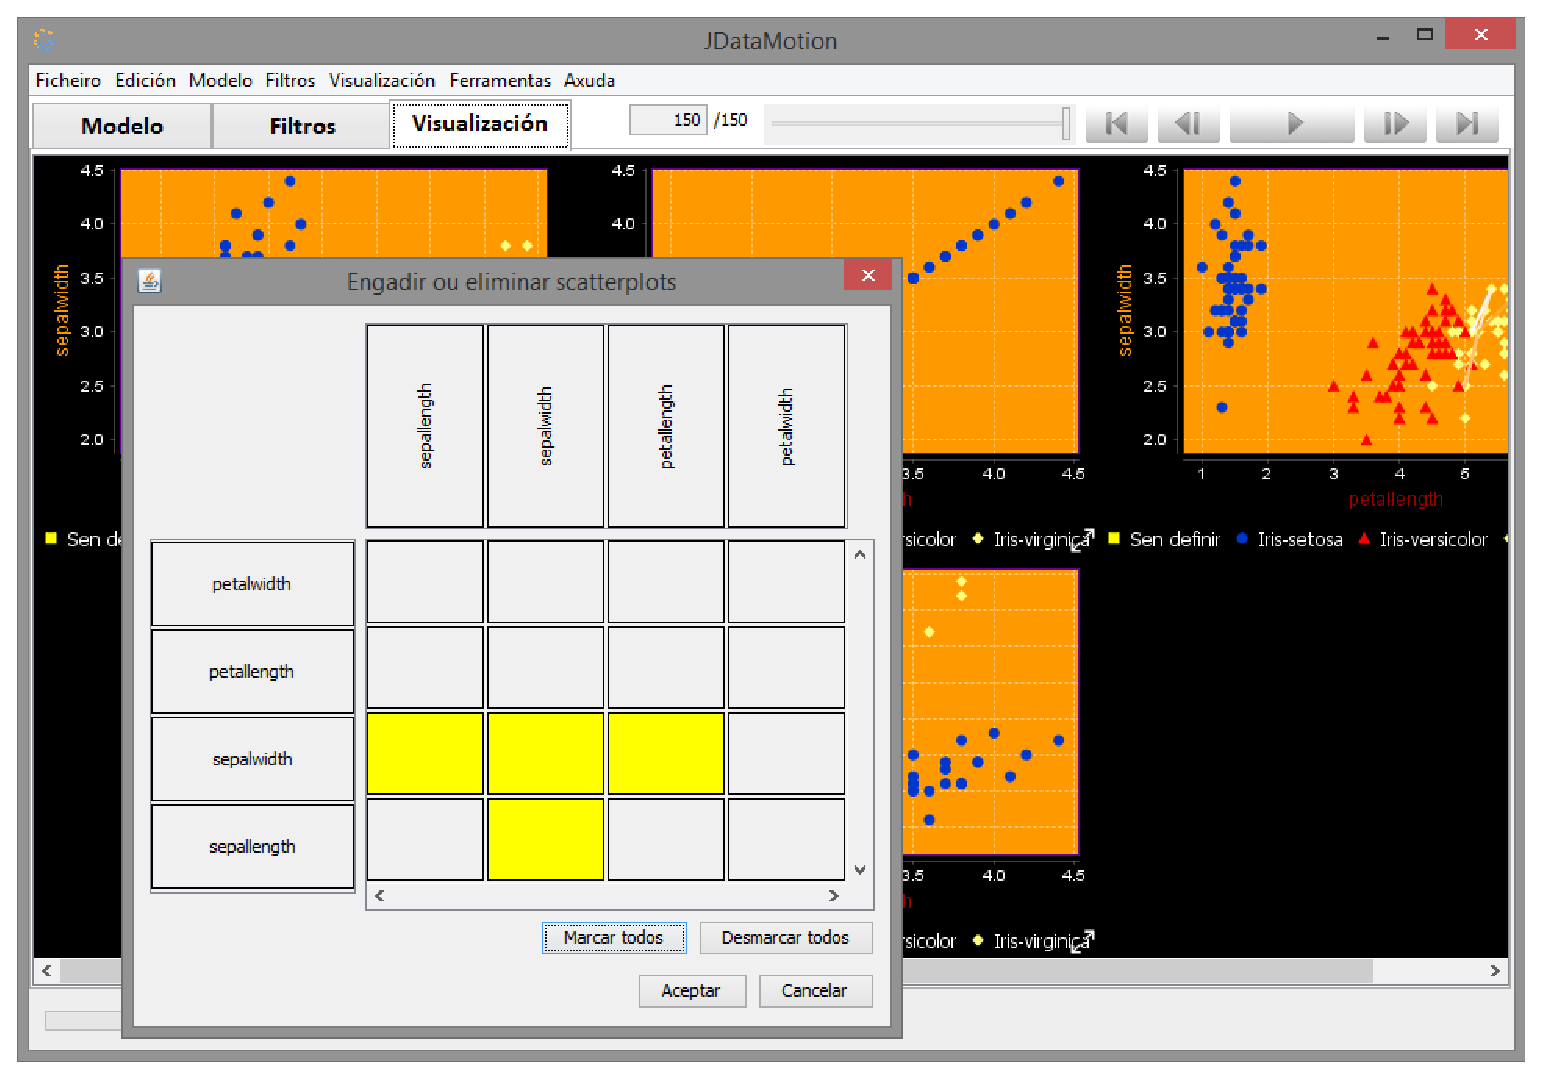
\includegraphics[width=\textwidth,height=\textheight,keepaspectratio]{figuras/RF1213}
\caption{Comprobación heurística do RF12}
\label{RF1213}
\end{figure}
\item[Resultado]
Correcto.
\end{description}

\subsubsection*{RF13}
\begin{description}
\item[Título] \hfill
Eliminar un diagrama de dispersión do menú de visualización
\item[Descrición] \hfill
A aplicación debe permitir eliminar un diagrama de dispersión do menú de visualización.
\item[Importancia] \hfill
Esencial
\item[Tipo de proba] \hfill
Avaliación heurística
\item[Descrición]
Consideramos que xa se esta visualizando algún scatterplot. Na barra de menús, iremos a Visualización \textgreater{} Engadir ou eliminar scatterplots e desmarcamos da matriz os elementos que queremos quitar da visualización.
\begin{figure}
\centering
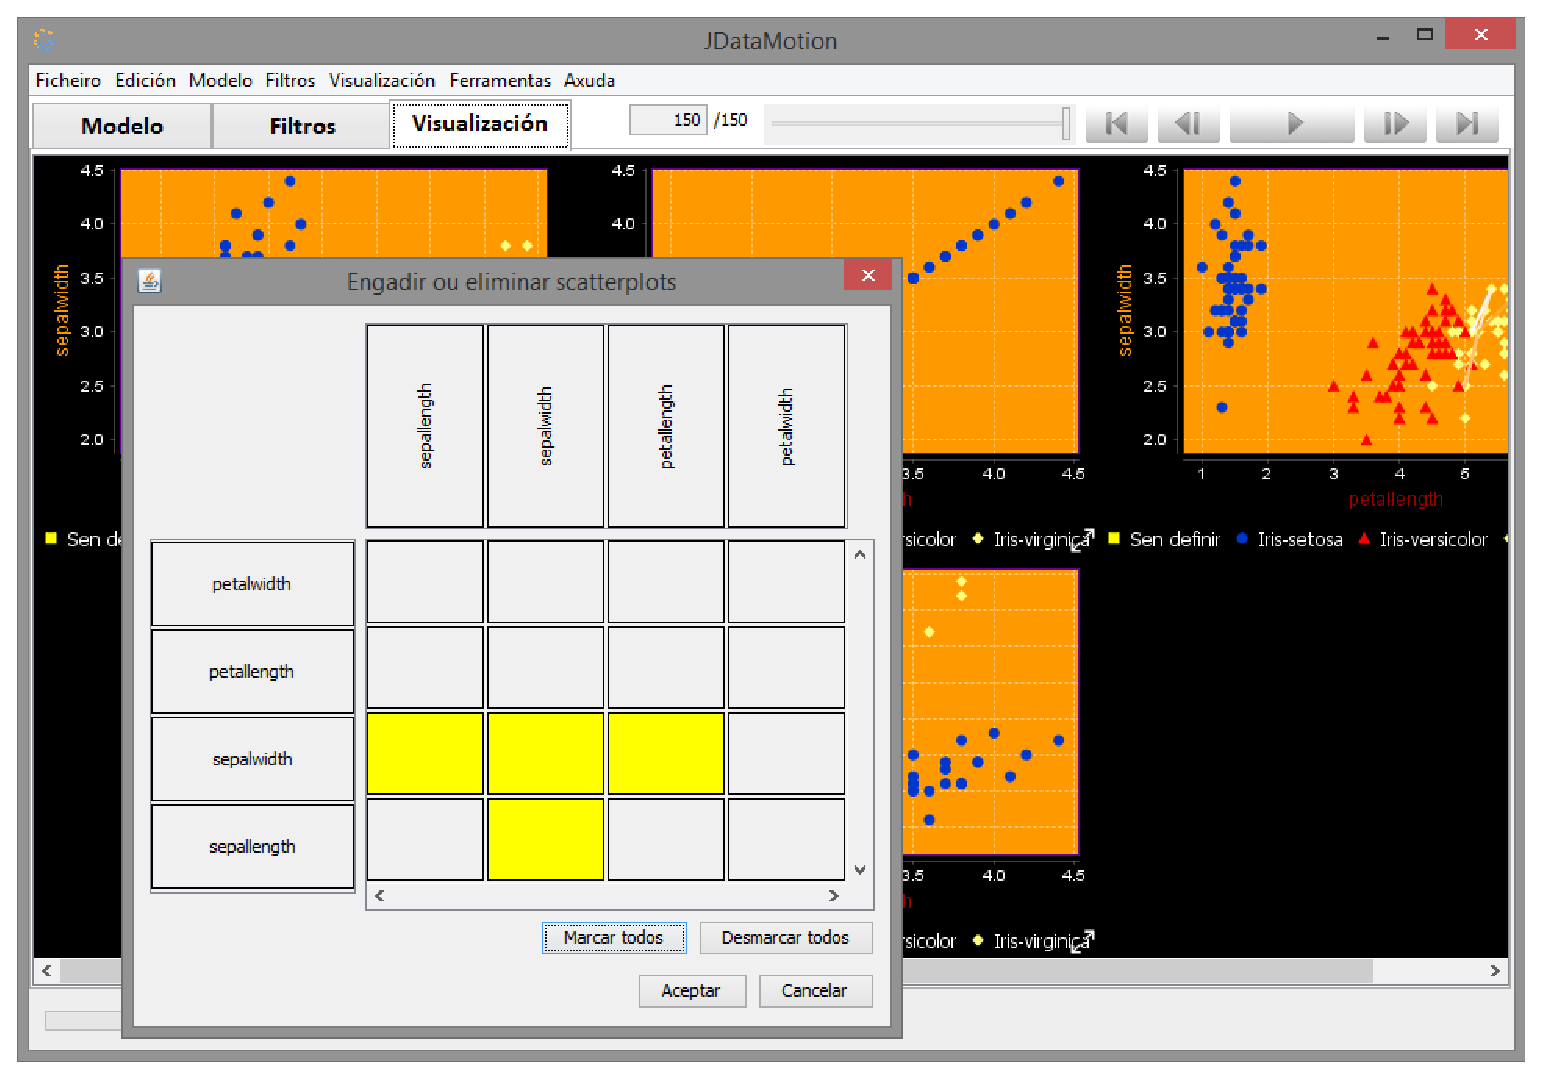
\includegraphics[width=\textwidth,height=\textheight,keepaspectratio]{figuras/RF1213}
\caption{Comprobación heurística do RF13}
\label{RF1213}
\end{figure}
\item[Resultado]
Correcto.
\end{description}

\subsubsection*{RF14}
\begin{description}
\item[Título] \hfill
Configurar diagramas de dispersión do menú de visualización
\item[Descrición] \hfill
A aplicación debe permitir especificar para os diagramas de dispersión do menú de visualización a súa configuración, respecto a que parámetros se representarán en cada un dos eixos ou si as cores e formas dos puntos se desexan usar para representar algún atributo nominal.
\item[Importancia] \hfill
Esencial
\item[Tipo de proba] \hfill
Avaliación heurística
\item[Descrición]
Para configurar os atributos representados en cada eixo está a matriz e3 selección de Visualización \textgreater{} Engadir ou eliminar scatterplots. (ver RF12 e RF13). Para representar un atributo de clase por medio de cores e formas diferentes, só temos que seleccionalo en Visualización \textgreater{} Establecer atributo nominal representado. Ao aceptar podemos apreciar o resultado.
\begin{figure}
\centering
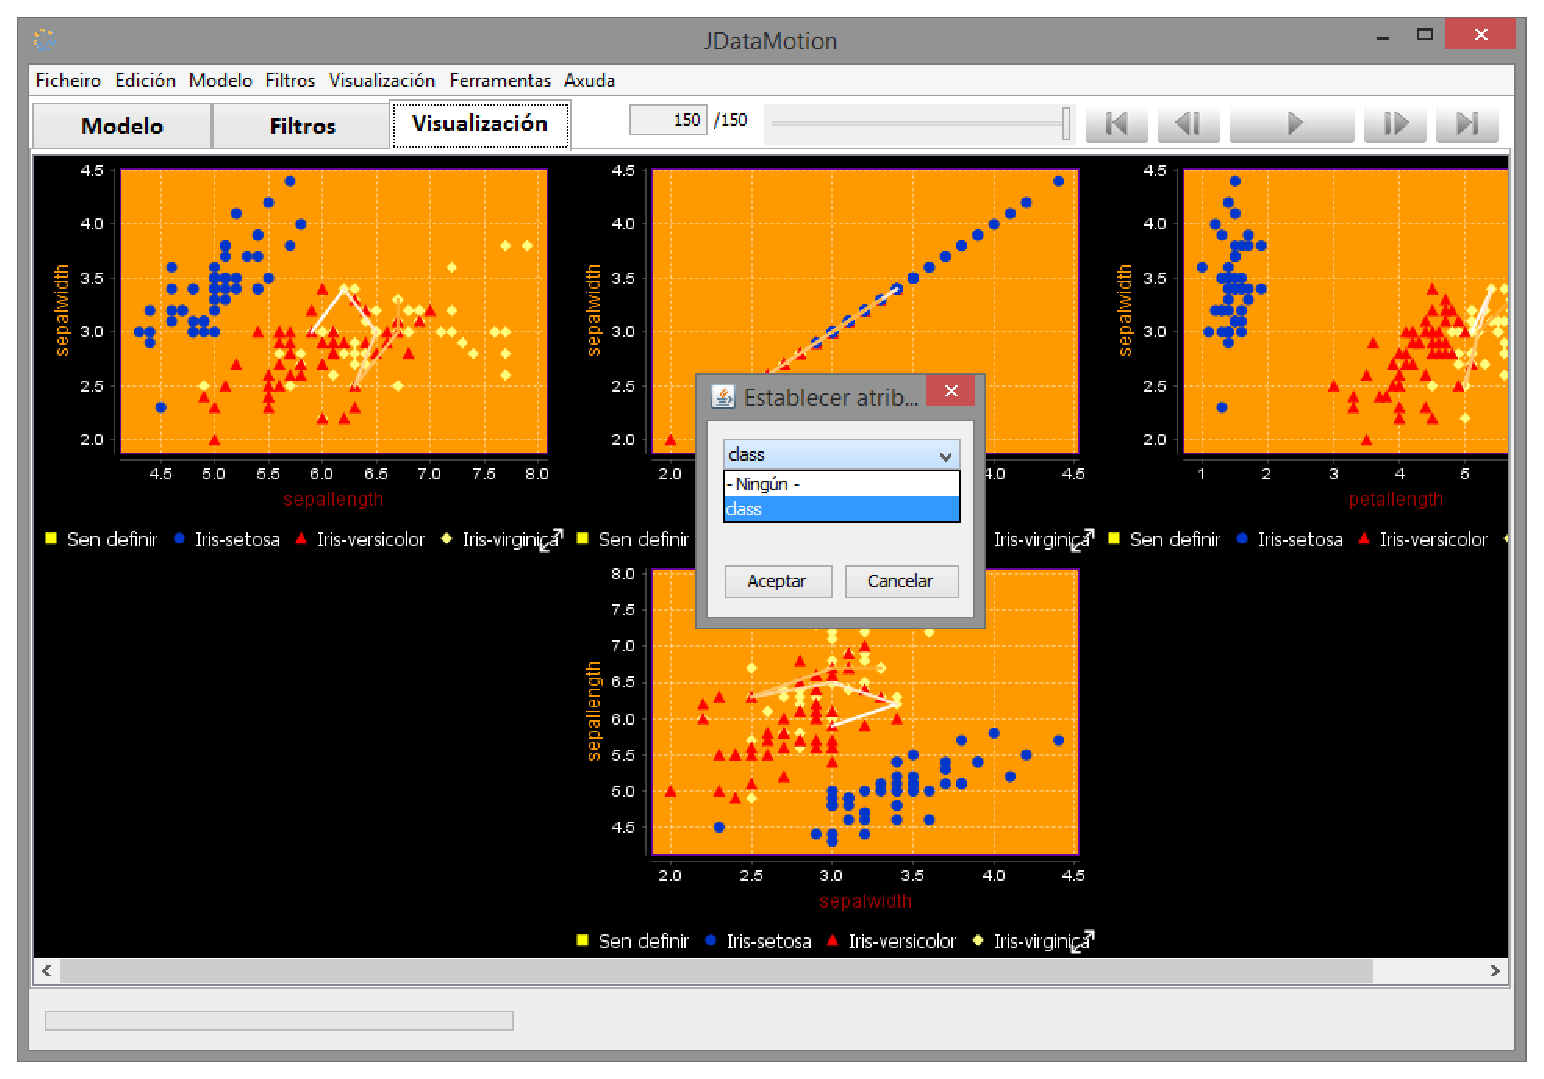
\includegraphics[width=\textwidth,height=\textheight,keepaspectratio]{figuras/RF14}
\caption{Comprobación heurística do RF14}
\label{RF14}
\end{figure}
\item[Resultado]
Correcto.
\end{description}

\subsubsection*{RF15}
\begin{description}
\item[Título] \hfill
Detallar punto seleccionado dentro do diagrama de dispersión
\item[Descrición] \hfill
Cada punto dos diagramas de dispersión pode ser seleccionado para ver nun apartado os seus detalles (todos os seus atributos).
\item[Importancia] \hfill
Esencial
\item[Tipo de proba] \hfill
Avaliación heurística
\item[Descrición]
Tendo algún diagrama representado podemos apreciar este efecto pulsando preto de calquera punto. Abrirase un menú que detalle o punto seleccionado, ou unha lista deles (puntos solapados).
\begin{figure}
\centering
\includegraphics[width=\textwidth,height=\textheight,keepaspectratio]{figuras/RF1516}
\caption{Comprobación heurística do RF15}
\label{RF1516}
\end{figure}
\item[Resultado]
Correcto.
\end{description}

\subsubsection*{RF16}
\begin{description}
\item[Título] \hfill
Resaltar punto en diagramas de dispersión
\item[Descrición] \hfill
Cada punto seleccionalo dentro dun diagrama de dispersión resaltarase tanto nel coma en todos os demais diagramas de dispersión (que plasmarán outras proxeccións do mesmo punto).
\item[Importancia] \hfill
Esencial
\item[Tipo de proba] \hfill
Avaliación heurística
\item[Descrición]
Tendo algúns diagramas representados podemos apreciar este efecto pulsando nun punto no que haxa algún outro punto coincidindo nesa mesma posición (puntos solapados). As proyeccións desos puntos noutros diagramas tamén se resaltan, mantendo o mesmo color as que referencian a mesma instancia.
\begin{figure}
\centering
\includegraphics[width=\textwidth,height=\textheight,keepaspectratio]{figuras/RF1516}
\caption{Comprobación heurística do RF16}
\label{RF1516}
\end{figure}
\item[Resultado]
Correcto.
\end{description}

\subsubsection*{RF17}
\begin{description}
\item[Título] \hfill
Desprazar a ventá de visualización por arrastre de cada diagrama de dispersión
\item[Descrición] \hfill
Para cada diagrama de dispersión poderemos usar unha ferramenta ``man'' para desprazar a ventá polo diagrama de dispersión.
\item[Importancia] \hfill
Esencial
\item[Tipo de proba] \hfill
Avaliación heurística
\item[Descrición]
Tendo algún diagrama representado podemos apreciar este efecto pulsando a tecla Control e arrastrando co rato un diagrama de dispersión. Veremos como a ventá que enfoca o gráfico se despraza na dirección que marquemos.
\begin{figure}
\centering
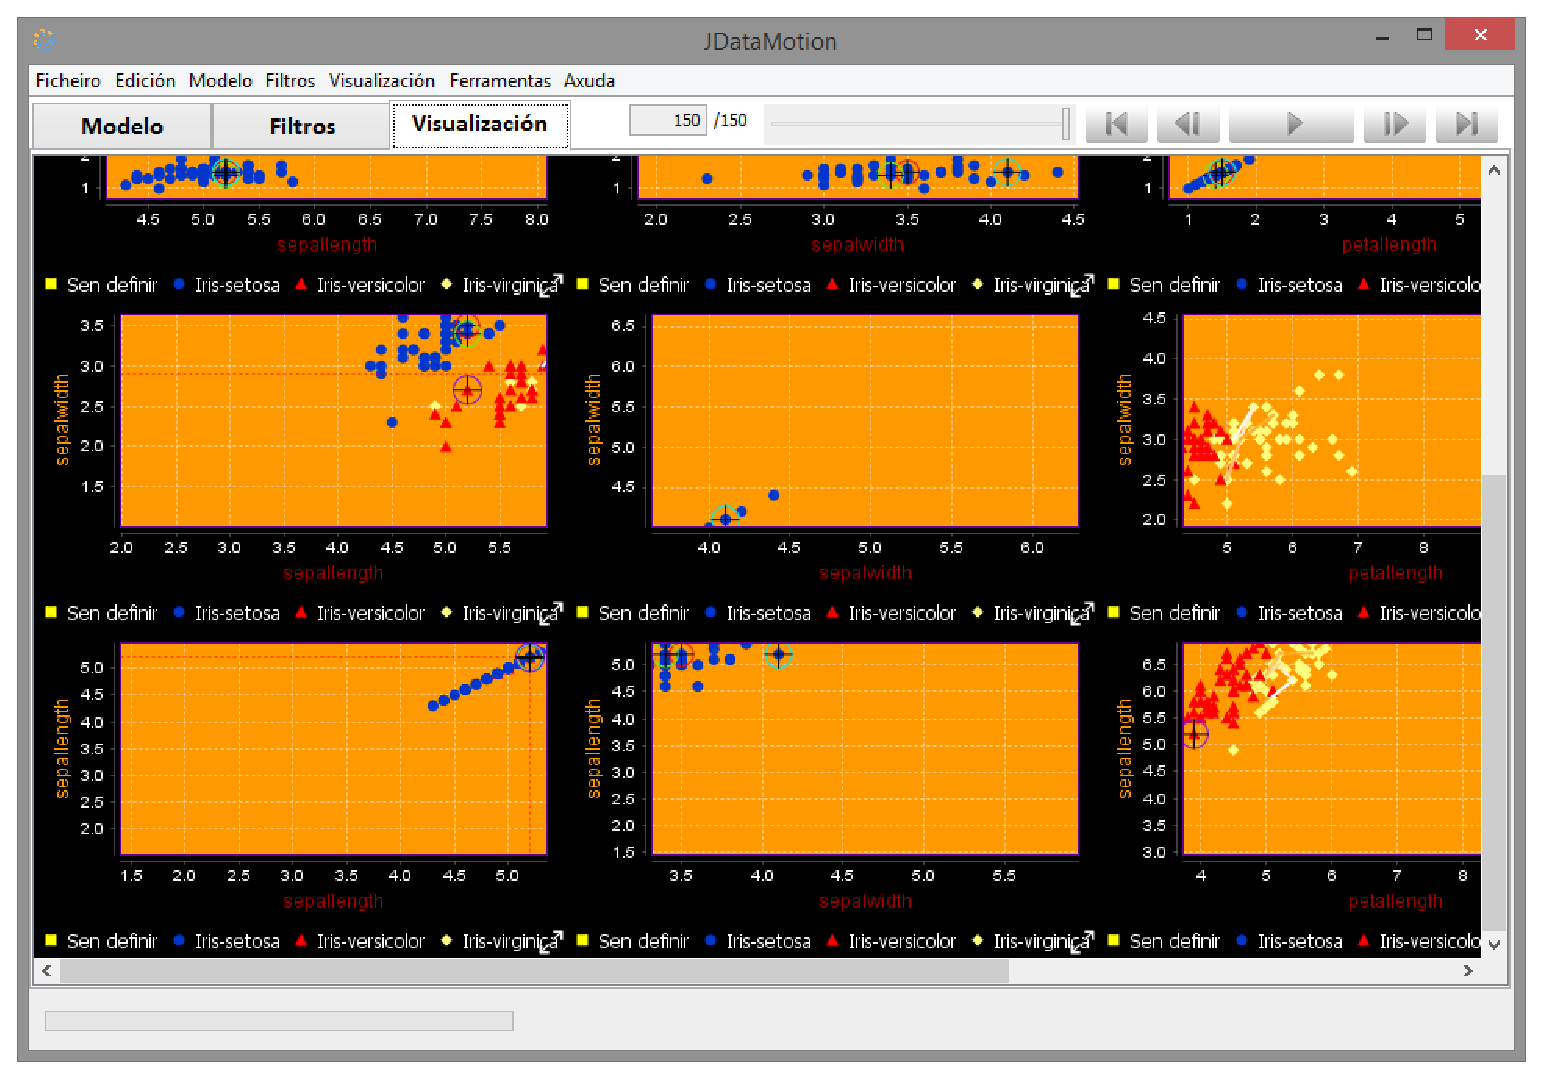
\includegraphics[width=\textwidth,height=\textheight,keepaspectratio]{figuras/RF17}
\caption{Comprobación heurística do RF17}
\label{RF17}
\end{figure}
\item[Resultado]
Correcto.
\end{description}

\subsubsection*{RF18}
\begin{description}
\item[Título] \hfill
Escalar a ventá de visualización de cada diagrama de dispersión
\item[Descrición] \hfill
Para cada diagrama de dispersión poderemos usar unha ferramenta de escalado da ventá para facer zoom no diagrama de dispersión.
\item[Importancia] \hfill
Esencial
\item[Tipo de proba] \hfill
Avaliación heurística
\item[Descrición]
Tendo algún diagrama representado podemos apreciar este efecto colocando o cursor enriba dun diagrama e xirando a roda do rato. Veremos como a ventá de visualización do diagrama escala. Tamén se pode probar pulsando co botón secundario nun diagrama e seleccionando unha opción dentro de Acercar ou Alonxar.
\begin{figure}
\centering
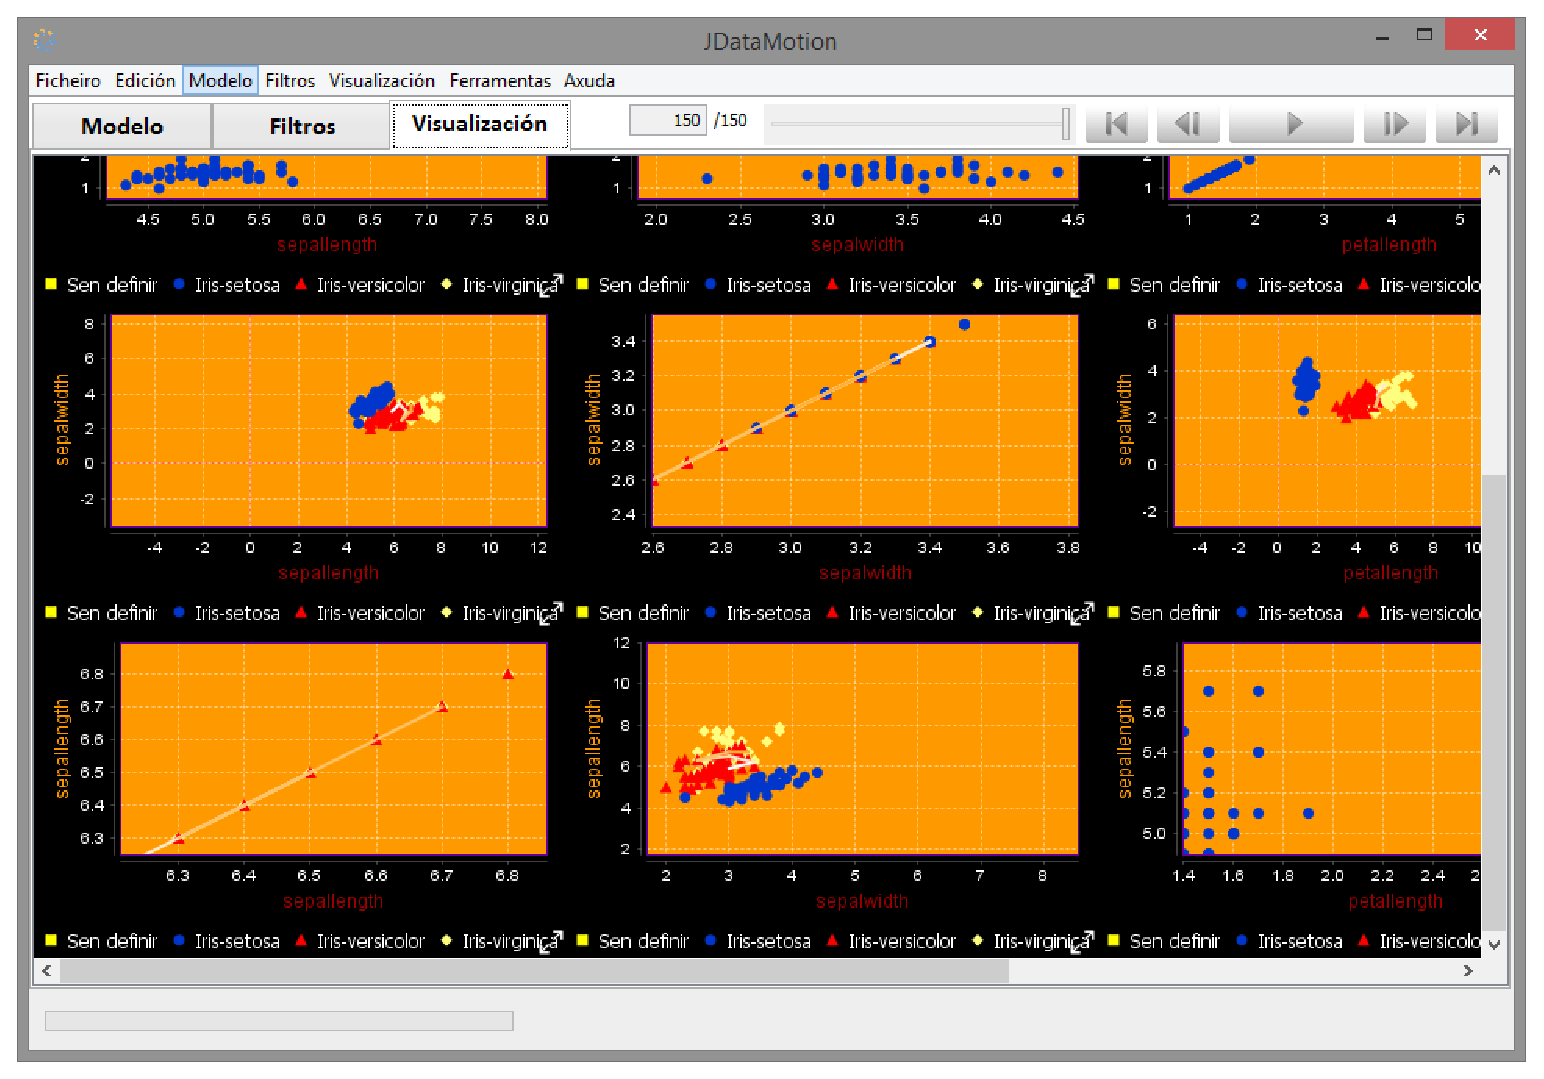
\includegraphics[width=\textwidth,height=\textheight,keepaspectratio]{figuras/RF18}
\caption{Comprobación heurística do RF18}
\label{RF18}
\end{figure}
\item[Resultado]
Correcto.
\end{description}

\subsubsection*{RF19}
\begin{description}
\item[Título] \hfill
Escalar e reposicionar dinamicamente
\item[Descrición] \hfill
Para cada diagrama de dispersión permitirase que a ventá de visualización que o enfoca se adapte dinamicamente ao conxunto de datos representados (movéndose, afastándose e aproximándose para englobar todos os datos).
\item[Importancia] \hfill
Esencial
\item[Tipo de proba] \hfill
Avaliación heurística
\item[Descrición]
Tendo algún diagrama representado podemos apreciar este efecto colocando o cursor enriba dun diagrama e xirando a roda do rato. Veremos como a ventá de visualización do diagrama escala.
\begin{figure}
\centering
\includegraphics[width=\textwidth,height=\textheight,keepaspectratio]{figuras/RF19}
\caption{Comprobación heurística do RF19}
\label{RF19}
\end{figure}
\item[Resultado]
Correcto.
\end{description}

\subsubsection*{RF20}
\begin{description}
\item[Título] \hfill
Reproducir a secuencia de datos
\item[Descrición] \hfill
A aplicación debe de permitir que a visualización dos diagramas de dispersión poida basearse na variable temporal (ou de orde) para reproducir a secuencia de datos, amosando os datos de cada diagrama de dispersión baixo unha secuencia de vídeo. Nesta secuencia engadiríase á visualización en cada instante a tupla de atributos asociada a esa marca temporal. 
\item[Importancia] \hfill
Esencial
\item[Tipo de proba] \hfill
Avaliación heurística
\item[Descrición]
Tendo algún diagrama representado, volvemos ao Modelo e seleccionamos un atributo numérico ou String (pero cun formato de tempo) pinchando nel co botón secundario. Marcámolo como índice temporal. Agora imos a Visualización \textgreater{} Configurar reprodución e personalizamos os valores que se amosan. Para que se teña en conta o índice temporal, seleccionaremos en Orde do modelo a opción ``Orde dos índices temporais numéricos'' ou ben ``Orde dos índices temporais numéricos ponderados'', en función de si o índice temporal expresa só orde ou unha duración relativa, respectivamente. Con todo isto, ao premer no botón de reprodución do menú Visualización comezaremos a ver a secuencia de puntos avanzar da forma que acabamos de configurar.
\begin{figure}
\centering
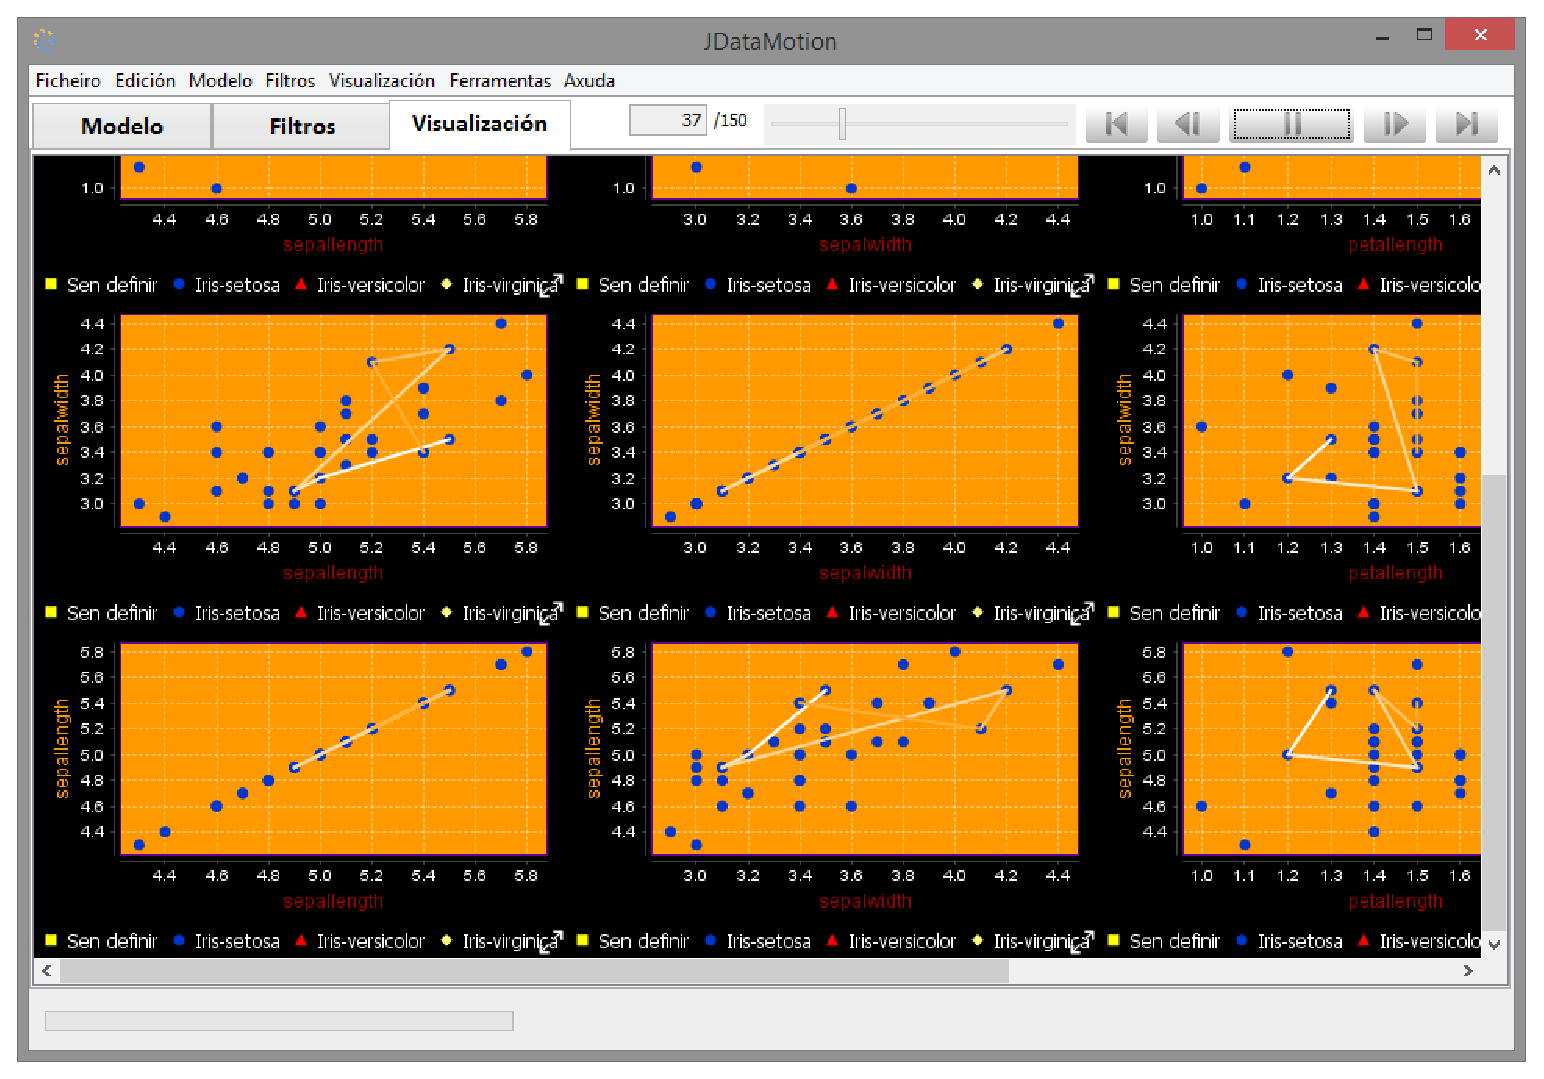
\includegraphics[width=\textwidth,height=\textheight,keepaspectratio]{figuras/RF202122}
\caption{Comprobación heurística do RF20}
\label{RF202122}
\end{figure}
\item[Resultado]
Correcto.
\end{description}

\subsubsection*{RF21}
\begin{description}
\item[Título] \hfill
Representar estela
\item[Descrición] \hfill
A aplicación debe de permitir que cada novo punto pintado se ligue ao último representado no diagrama de dispersión por medio dunha liña recta.
\item[Importancia] \hfill
Esencial
\item[Tipo de proba] \hfill
Avaliación heurística
\item[Descrición]
Tendo algún diagrama representado, imos a Visualización \textgreater{} Configurar reprodución e asegurámonos de que o valor da lonxitude de estela non sexa 0. Entón premendo no botón de reproducir veremos que a estela abarcará o número de puntos especificado, tendo a súa cabeza no último punto que se visualiza en cada momento.
\begin{figure}
\centering
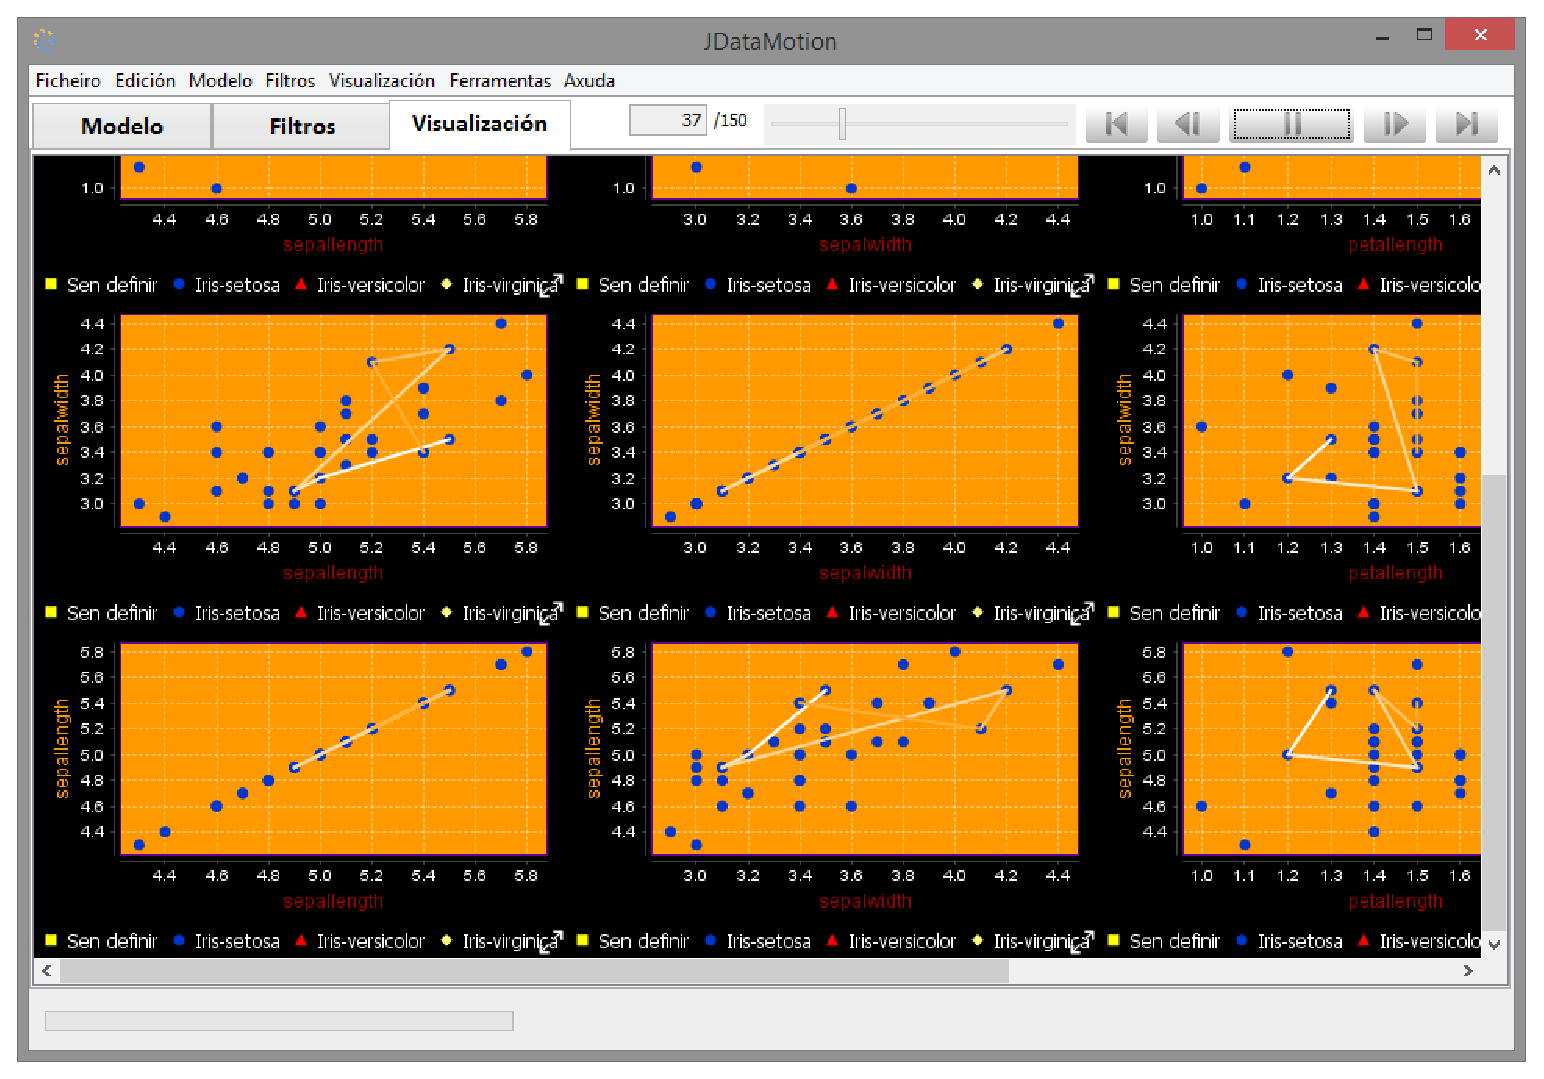
\includegraphics[width=\textwidth,height=\textheight,keepaspectratio]{figuras/RF202122}
\caption{Comprobación heurística do RF21}
\label{RF202122}
\end{figure}
\item[Resultado]
Correcto.
\end{description}

\subsubsection*{RF22}
\begin{description}
\item[Título] \hfill
Difuminar estela ao longo da reprodución
\item[Descrición] \hfill
A aplicación debe permitir difuminar as estelas xa representadas a través do avance temporal.
\item[Importancia] \hfill
Esencial
\item[Tipo de proba] \hfill
Avaliación heurística
\item[Descrición]
Tendo algún diagrama representado, imos a Visualización \textgreater{} Configurar reprodución e asegurámonos de que o valor da lonxitude de estela sexa un número significativo. Entón premendo no botón de reproducir veremos que a estela abarcará o número de puntos especificado, tendo unha cor máis intensa nos tramos nos que une puntos máis recentes, e máis tenue naqueles con maior antigüidade.
\begin{figure}
\centering
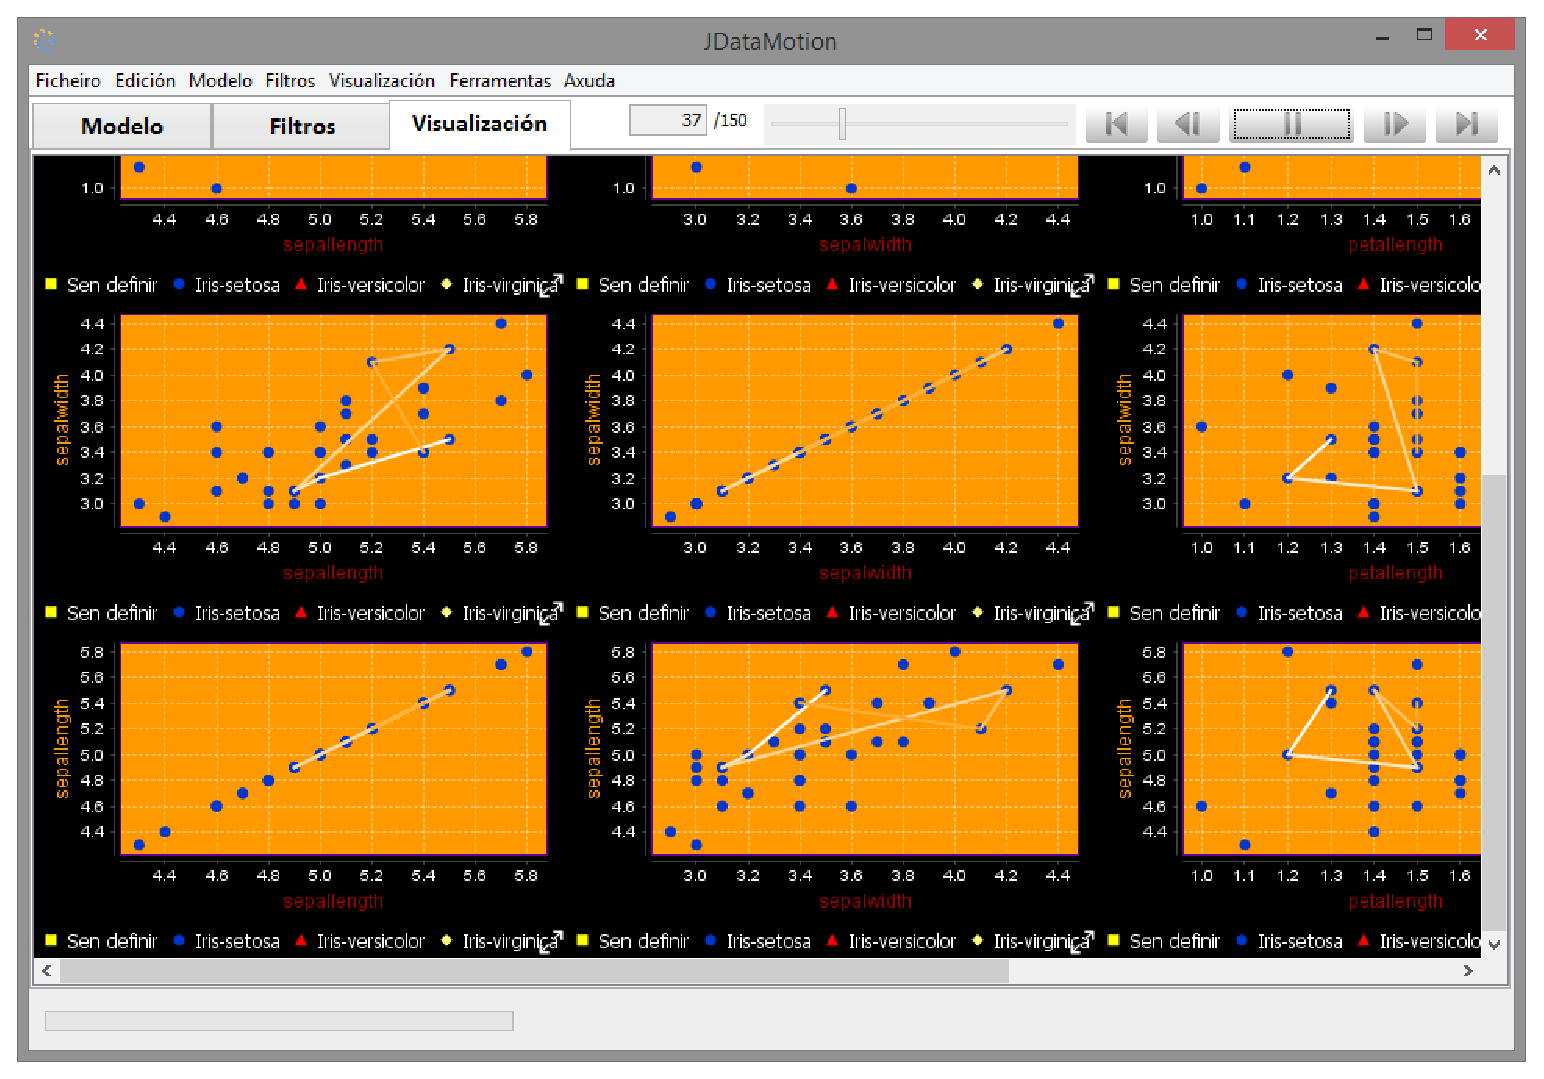
\includegraphics[width=\textwidth,height=\textheight,keepaspectratio]{figuras/RF202122}
\caption{Comprobación heurística do RF22}
\label{RF202122}
\end{figure}
\item[Resultado]
Correcto.
\end{description}

\subsubsection*{RF23}
\begin{description}
\item[Título] \hfill
Configurar a reprodución da secuencia de datos
\item[Descrición] \hfill
A aplicación debe de permitir que a visualización dos diagramas de dispersión sexa configurable en canto a tempo transcorrido entre marcas temporais. Para a reprodución usando marcas temporais ponderadas, este tempo representará a separación entre as dúas marcas temporais mais próximas (tempo mínimo). Ademáis débese poder especificar o número de marcas temporais que durará o difuminado dos puntos que se ploteen, de xeito que durante ese intervalo cada punto se vaia difuminando ata desaparecer. Pode ser igual a 0 para que os puntos non se difuminen.
\item[Importancia] \hfill
Esencial
\item[Tipo de proba] \hfill
Avaliación heurística
\item[Descrición]
Tendo algún diagrama representado, volvemos ao Modelo e seleccionamos un atributo numérico ou String (pero cun formato de tempo) pinchando nel co botón secundario. Marcámolo como índice temporal. Agora imos a Visualización \textgreater{}. Para que se teña en conta o índice temporal, seleccionaremos en Orde do modelo a opción ``Orde dos índices temporais numéricos ponderados''. Con todo isto, ao premer no botón de reprodución do menú Visualización comezaremos a ver a secuencia de puntos avanzar da forma que acabamos de configurar. O difuminado dos puntos non se pode probar porque non foi implementado todavía (debido a unha restricción das estruturas do Dataset que non permitían a reprodución cara atrás).
\begin{figure}
\centering
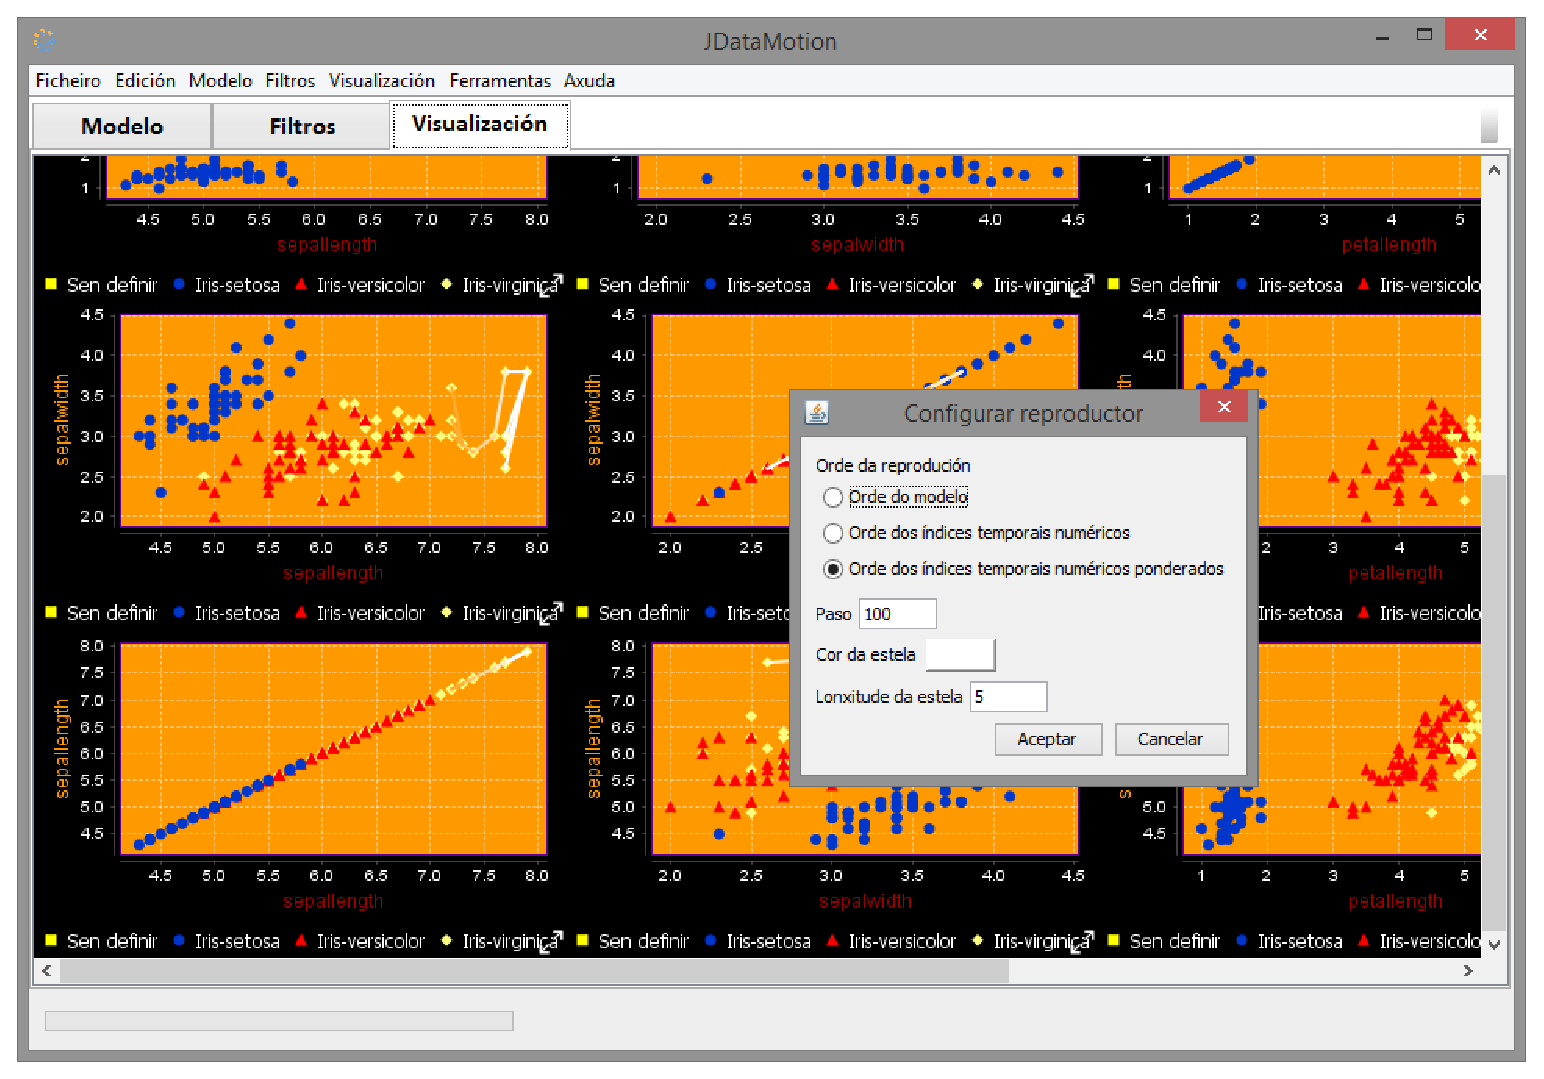
\includegraphics[width=\textwidth,height=\textheight,keepaspectratio]{figuras/RF23}
\caption{Comprobación heurística do RF23}
\label{RF23}
\end{figure}
\item[Resultado]
Correcto.
\end{description}

\subsubsection*{RF24}
\begin{description}
\item[Título] \hfill
Pausar a reprodución
\item[Descrición] \hfill
A aplicación debe permitir parar a reprodución na marca de tempo na que se atope ao executar esta acción, mantendo as visualizacións para ese momento.
\item[Importancia] \hfill
Esencial
\item[Tipo de proba] \hfill
Avaliación heurística
\item[Descrición]
Tendo algún diagrama representado e coa reprodución en curso, prememos outra vez no botón de reprodción (que agora terá un símbolo de dúas barras verticais paralelas). Comprobamos que todos os diagramas deteron a súa reprodución.
\begin{figure}
\centering
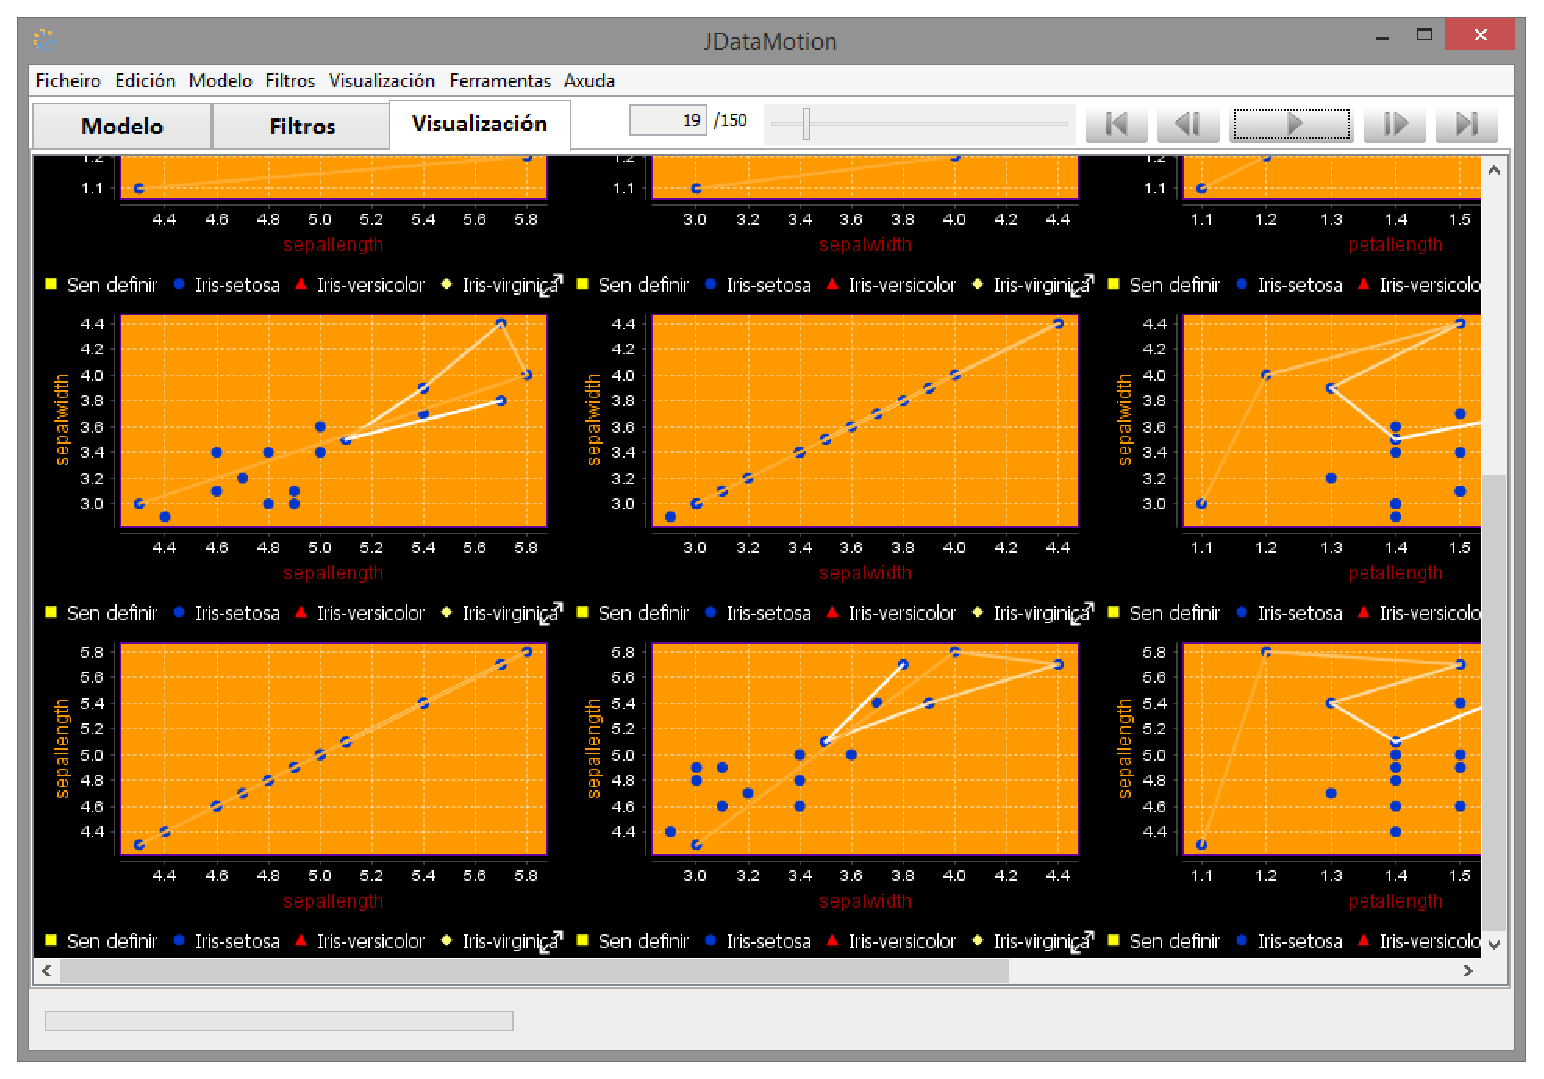
\includegraphics[width=\textwidth,height=\textheight,keepaspectratio]{figuras/RF24}
\caption{Comprobación heurística do RF24}
\label{RF24}
\end{figure}
\item[Resultado]
Correcto.
\end{description}

\subsubsection*{RF25}
\begin{description}
\item[Título] \hfill
Ir a un determinado instante dentro do intervalo temporal da reprodución
\item[Descrición] \hfill
A aplicación debe permitir situarse directamente sobre un instante de tempo, mantendo a reprodución pausada sobre esa marca temporal, e visualizando os diagramas de dispersión tal e como deben estar nese momento.
\item[Importancia] \hfill
Esencial
\item[Tipo de proba] \hfill
Avaliación heurística
\item[Descrición]
Tendo algún diagrama representado, observamos o desprazador que está no menú de Visualización, ao lado dos demais botóns de reprodución. Arrastramos o seu pivote por todo o ancho e observamos como aparecen (cando nos movemos acara a dereita) ou se agochan (cando nos movemos cara a esquerda) puntos en todos os diagramas. Soltando o pivote nunha posición a reprodución establécese nela, seguindo a partir de aí no caso de reanudarse.
\begin{figure}
\centering
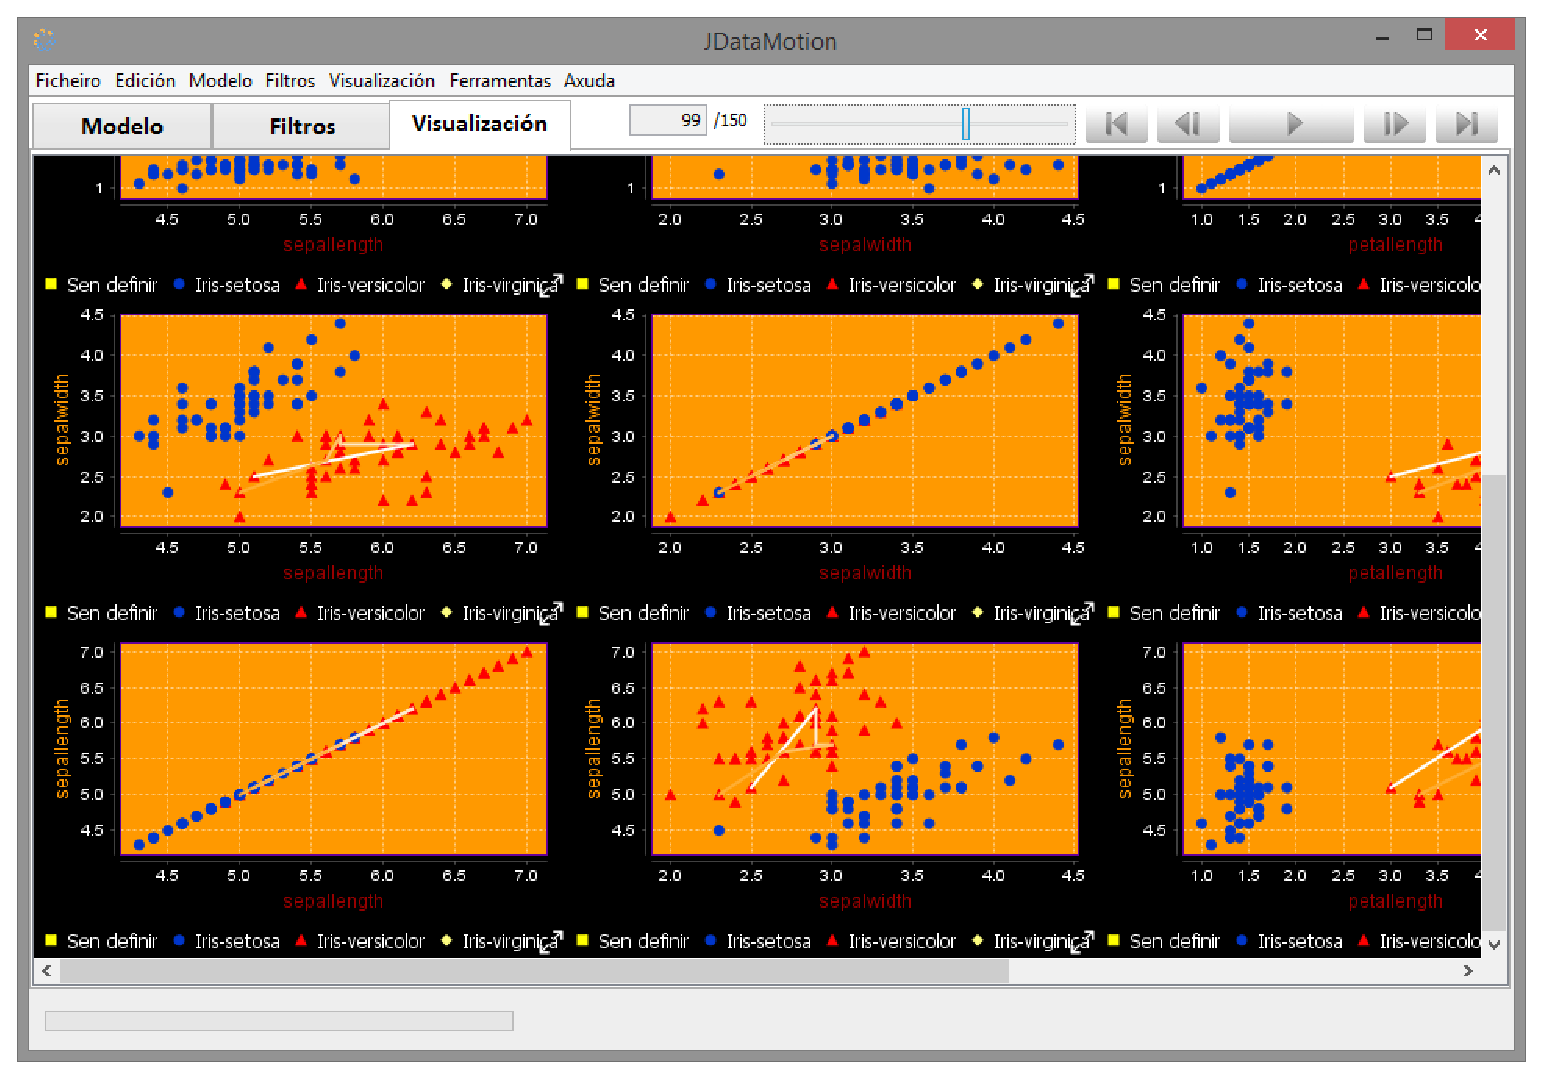
\includegraphics[width=\textwidth,height=\textheight,keepaspectratio]{figuras/RF25}
\caption{Comprobación heurística do RF25}
\label{RF25}
\end{figure}
\item[Resultado]
Correcto.
\end{description}

\subsubsection*{RF26}
\begin{description}
\item[Título] \hfill
Insertar filtros para os datos do experimento
\item[Descrición] \hfill
A aplicación debe permitir engadir unha serie de filtros que se aplicarán de xeito secuencial sobre a secuencia de datos coa que se esté a traballar. Chamarémoslle ``secuencia de filtros'' a esta secuencia.
\item[Importancia] \hfill
Esencial
\item[Tipo de proba] \hfill
Test implementado en JUnit.
\item[Nome do test] \hfill
TestRF2628
\item[Código fonte]
\begin{lstlisting}
    public void test() {
        Modelo modelo = new Modelo();
        Vista vista = new Vista();
        vista.inicializar(modelo, false);
        Controlador.setDebug(true);
        String resource = "example01.arff";
        IFilter filtro = new FiltroLimite();
        Double maximo = 15.0;
        int columna = 1;
        StringParameter sp1 = new StringParameter(), sp2 = new StringParameter();
        DoubleParameter sp3 = new DoubleParameter();
        sp1.setValue(recursosIdioma.getString("limiteValor"));
        sp2.setValue(recursosIdioma.getString("cotaSuperior"));
        sp3.setValue(maximo);
        try {
            String pathEntrada = new URI(getClass().getResource(resource).toString()).getPath();
            ComparableInstances is1 = ValidFileLoading.loadARFF(pathEntrada);
            modelo.setComparableInstances(new ComparableInstances(is1));
            vista.getControlador().manexarEvento(Controlador.ENGADIR_FILTRO, new Object[]{0, filtro});
            modelo.getFiltro(0).getParameters().put(recursosIdioma.getString("tipoLimite"), sp1);
            modelo.getFiltro(0).getParameters().put(recursosIdioma.getString("tipoCota"), sp2);
            modelo.getFiltro(0).getParameters().put(recursosIdioma.getString("valor"), sp3);
            modelo.getFiltro(0).setIndiceAtributoFiltrado(columna);
            boolean todosMenores = true;
            Enumeration<Instance> e = modelo.getComparableInstancesFiltradas().enumerateInstances();
            while (e.hasMoreElements()) {
                Instance i = e.nextElement();
                if (i.value(columna) > maximo) {
                    todosMenores = false;
                }
            }
            assertEquals(todosMenores, true);
        } catch (URISyntaxException ex) {
            Logger.getLogger(getClass().getName()).log(Level.SEVERE, null, ex);
        }
    }
\end{lstlisting}
\item[Descrición]
Este test comproba si ao enviar un evento de tipo ENGADIR\_FILTRO e configurar o filtro en cuestión, se aprecian os seus efectos no método getComparableInstancesFiltradas. En concreto pasaráselle un FiltroLimite que poña a 15 todos os valores da 2º columna que o superen. Estes datos constitúen a configuración do filtro, a cal tamén se proba neste método.
\item[Resultado]
Correcto.
\end{description}

\subsubsection*{RF27}
\begin{description}
\item[Título] \hfill
Eliminar un filtro para os datos do experimento
\item[Descrición] \hfill
A aplicación debe permitir eliminar un determinado filtro dentro da secuencia de filtros.
\item[Importancia] \hfill
Esencial
\item[Tipo de proba] \hfill
Test implementado en JUnit.
\item[Nome do test] \hfill
TestRF2627
\item[Código fonte]
\begin{lstlisting}
public void test() {
        Modelo modelo = new Modelo();
        Vista vista = new Vista();
        vista.inicializar(modelo, false);
        Controlador.setDebug(true);
        String resource = "example01.arff";
        IFilter filtro = new FiltroLimite();
        Double maximo = 15.0;
        int columna = 1;
        StringParameter sp1 = new StringParameter(), sp2 = new StringParameter();
        DoubleParameter sp3 = new DoubleParameter();
        sp1.setValue(recursosIdioma.getString("limiteValor"));
        sp2.setValue(recursosIdioma.getString("cotaSuperior"));
        sp3.setValue(maximo);
        try {
            String pathEntrada = new URI(getClass().getResource(resource).toString()).getPath();
            ComparableInstances is1 = ValidFileLoading.loadARFF(pathEntrada);
            modelo.setComparableInstances(new ComparableInstances(is1));
            vista.getControlador().manexarEvento(Controlador.ENGADIR_FILTRO, new Object[]{0, filtro});
            modelo.getFiltro(0).getParameters().put(recursosIdioma.getString("tipoLimite"), sp1);
            modelo.getFiltro(0).getParameters().put(recursosIdioma.getString("tipoCota"), sp2);
            modelo.getFiltro(0).getParameters().put(recursosIdioma.getString("valor"), sp3);
            modelo.getFiltro(0).setIndiceAtributoFiltrado(columna);
            vista.getControlador().manexarEvento(Controlador.ELIMINAR_FILTRO, 0);
            ComparableInstances is2 = modelo.getComparableInstancesFiltradas();
            assertEquals(is1, is2);
        } catch (URISyntaxException ex) {
            Logger.getLogger(getClass().getName()).log(Level.SEVERE, null, ex);
        }
    }
\end{lstlisting}
\item[Descrición]
Este test comproba si despois de eliminar un filtro que engadimos e configuramos, obtemos unhas ComparableInstances equivalentes ao estado inicial do experimento, o que significa que o evento ELIMINAR\_FILTRO e ENGADIR\_FILTRO funcionan correctamente.
\item[Resultado]
Correcto.
\end{description}

\subsubsection*{RF28}
\begin{description}
\item[Título] \hfill
Configurar filtros para os datos do experimento
\item[Descrición] \hfill
A aplicación debe permitir seleccionar un determinado filtro dentro da secuencia de filtros para modificar a regla de filtrado implícita.
\item[Importancia] \hfill
Esencial
\item[Nome do test] \hfill
TestRF2628
\item[Descrición]
Ver TestRF2628.
\item[Resultado]
Correcto.
\end{description}

\subsubsection*{RF29}
\begin{description}
\item[Título] \hfill
Gardar unha secuencia de filtros do experimento
\item[Descrición] \hfill
A aplicación debe permitir gardar unha secuencia de filtros, non necesariamente correlativos, dentro dos que se estean aplicando sobre o experimento. Esta secuencia pode comprender tanto un só filtro como a secuencia de filtros enteira.
\item[Importancia] \hfill
Esencial
\item[Tipo de proba] \hfill
Test implementado en JUnit.
\item[Nome do test] \hfill
TestRF262930
\item[Código fonte]
\begin{lstlisting}
public void test() {
        Modelo modelo = new Modelo();
        Vista vista = new Vista();
        vista.inicializar(modelo, false);
        Controlador.setDebug(true);
        String resource = "example01.arff";
        String archivoSesion = "tempFiltros.jdmf";
        IFilter filtro = new FiltroLimite();
        Double maximo = 15.0;
        int columna = 1;
        StringParameter sp1 = new StringParameter(), sp2 = new StringParameter();
        DoubleParameter sp3 = new DoubleParameter();
        sp1.setValue(recursosIdioma.getString("limiteValor"));
        sp2.setValue(recursosIdioma.getString("cotaSuperior"));
        sp3.setValue(maximo);
        try {
            String pathSaida = new URI(getClass().getResource(".").toString()).getPath() + archivoSesion;
            String pathEntrada = new URI(getClass().getResource(resource).toString()).getPath();
            ComparableInstances is1 = ValidFileLoading.loadARFF(pathEntrada);
            modelo.setComparableInstances(new ComparableInstances(is1));
            vista.getControlador().manexarEvento(Controlador.ENGADIR_FILTRO, new Object[]{0, filtro});
            modelo.getFiltro(0).getParameters().put(recursosIdioma.getString("tipoLimite"), sp1);
            modelo.getFiltro(0).getParameters().put(recursosIdioma.getString("tipoCota"), sp2);
            modelo.getFiltro(0).getParameters().put(recursosIdioma.getString("valor"), sp3);
            modelo.getFiltro(0).setIndiceAtributoFiltrado(columna);
            vista.getControlador().manexarEvento(Controlador.EXPORTAR_FILTROS, new Object[]{pathSaida, new Integer[]{0}});
            vista.getControlador().manexarEvento(Controlador.IMPORTAR_FILTROS, pathSaida);
            boolean valido = true;
            for (Entry<String, Parameter> entry : modelo.getFiltro(0).getParameters().entrySet()) {
                if (!modelo.getFiltro(0).getParameters().get(entry.getKey()).getValue().equals(modelo.getFiltro(1).getParameters().get(entry.getKey()).getValue())) {
                    valido = false;
                    break;
                }
            }
            if (valido == true
                    && (!modelo.getFiltro(0).getFiltro().getClass().equals(modelo.getFiltro(1).getFiltro().getClass())
                    || modelo.getFiltro(0).getIndiceAtributoFiltrado() != columna
                    || modelo.getFiltro(1).getIndiceAtributoFiltrado() != null)) {
                valido = false;
            }
            assertEquals(valido, true);
        } catch (URISyntaxException ex) {
            Logger.getLogger(getClass().getName()).log(Level.SEVERE, null, ex);
        }
    }
\end{lstlisting}
\item[Descrición]
Este test comproba que a exportación e importación de filtros acada os seus obxectivos. En concreto, os filtros deben ser da mesma clase, o filtro importado debeu perder o índice do atributo durante a exportación, e o resto de parámetros mantivéronse intactos durante o proceso.
\item[Resultado]
Correcto.
\end{description}

\subsubsection*{RF30}
\begin{description}
\item[Título] \hfill
Cargar unha secuencia de filtros para o experimento
\item[Descrición] \hfill
A aplicación debe permitir cargar do sistema de arquivos unha secuencia de filtros que se engadirá á cabeza da secuencia de filtros (a cal pode estar baleira). Esta secuencia tamén pode estar composta por un só filtro.
\item[Importancia] \hfill
Esencial
\item[Nome do test] \hfill
TestRF262930
\item[Descrición]
Ver TestRF262930.
\item[Resultado]
Correcto.
\end{description}

\subsubsection*{RF31}
\begin{description}
\item[Título] \hfill
Mover os filtros dentro da secuencia de filtros
\item[Descrición] \hfill
A aplicación debe permitir desprazar un filtro dentro da secuencia de filtros do experimento, de xeito que o orde de aplicación dos filtros varíe. O desprazamento realizarase inserindo o filtro en cuestión nunha nova posición.
\item[Importancia] \hfill
Esencial
\item[Tipo de proba] \hfill
Test implementado en JUnit.
\item[Nome do test] \hfill
TestRF2631
\item[Código fonte]
\begin{lstlisting}
public void test() {
        Modelo modelo = new Modelo();
        Vista vista = new Vista();
        vista.inicializar(modelo, false);
        Controlador.setDebug(true);
        String resource = "example01.arff";
        String archivoSesion = "tempFiltros.jdmf";
        IFilter filtro1 = new FiltroLimite();
        IFilter filtro2 = new FiltroNormalizacion();
        Double maximo = 15.0;
        int columna = 1;
        StringParameter sp1 = new StringParameter(), sp2 = new StringParameter();
        DoubleParameter sp3 = new DoubleParameter();
        sp1.setValue(recursosIdioma.getString("limiteValor"));
        sp2.setValue(recursosIdioma.getString("cotaSuperior"));
        sp3.setValue(maximo);
        try {
            String pathEntrada = new URI(getClass().getResource(resource).toString()).getPath();
            ComparableInstances is1 = ValidFileLoading.loadARFF(pathEntrada);
            modelo.setComparableInstances(new ComparableInstances(is1));
            vista.getControlador().manexarEvento(Controlador.ENGADIR_FILTRO, new Object[]{0, filtro1});
            modelo.getFiltro(0).getParameters().put(recursosIdioma.getString("tipoLimite"), sp1);
            modelo.getFiltro(0).getParameters().put(recursosIdioma.getString("tipoCota"), sp2);
            modelo.getFiltro(0).getParameters().put(recursosIdioma.getString("valor"), sp3);
            modelo.getFiltro(0).setIndiceAtributoFiltrado(columna);
            vista.getControlador().manexarEvento(Controlador.ENGADIR_FILTRO, new Object[]{1, filtro2});
            modelo.getFiltro(1).setIndiceAtributoFiltrado(columna);
            vista.getControlador().manexarEvento(Controlador.INTERCAMBIAR_FILTROS, new Object[]{0, 1});
            assertEquals(modelo.getFiltro(1).getFiltro().equals(filtro1) && modelo.getFiltro(0).getFiltro().equals(filtro2), true);
        } catch (URISyntaxException ex) {
            Logger.getLogger(getClass().getName()).log(Level.SEVERE, null, ex);
        }
    }
\end{lstlisting}
\item[Descrición]
Este test comproba que ao engadir dous filtros por medio do evento ENGADIR\_FILTRO e intercambialos por medio de INTERCAMBIAR\_FILTROS, cada un dos dous filtros está na posición que antes tiña o outro.
\item[Resultado]
Correcto.
\end{description}

\subsubsection*{RF32}
\begin{description}
\item[Título] \hfill
Configurar o menú de visualización
\item[Descrición] \hfill
A aplicación debe permitir cambiar os parámetros de visualización dos diagramas de dispersión que compoñen o menú de visualización, por exemplo, a cor das etiquetas e lendas, do fondo, dos eixos... ou a fonte, tamaño de letra...
\item[Importancia] \hfill
Optativa
\item[Tipo de proba] \hfill
Avaliación heurística
\item[Descrición]
Abrimos un ficheiro ARFF ou CSV e imos á lapela de Visualización. Podemos acceder ao menú de configuración gráfica pinchando co botón secundario nun diagrama ou mesmo no lenzo do menú. Sairá un menú contextual cunha opción chamada Propiedades, que abrirá o menú en cuestión.
Podemos comprobar como toda a configuración insertada se aplica ao experimento en canto prememos ``Aceptar''.
\begin{figure}
\centering
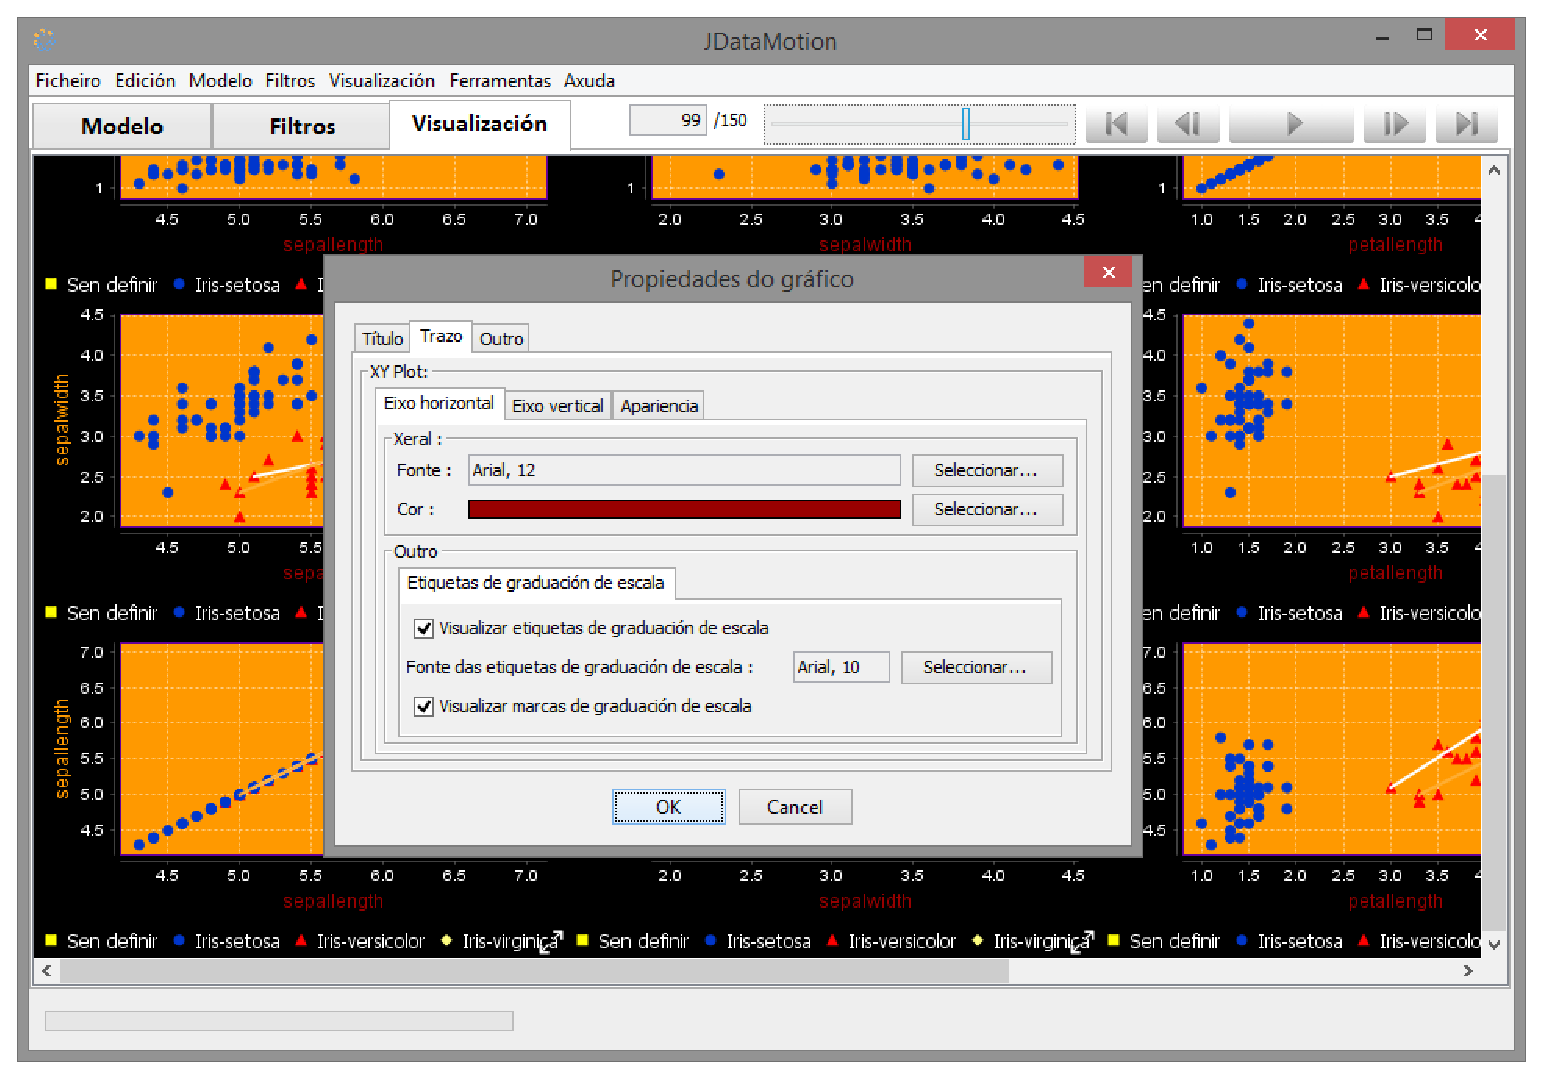
\includegraphics[width=\textwidth,height=\textheight,keepaspectratio]{figuras/RF32}
\caption{Comprobación heurística do RF32}
\label{RF32}
\end{figure}
\item[Resultado]
Correcto.
\end{description}

\subsection{Requisitos de calidade}

\subsubsection*{RC01}
\begin{description}
\item[Título] \hfill
Latencia mínima para o procesamento
\item[Descrición] \hfill
A aplicación debe responder nun tempo razoable ás operacións executadas polo usuario, e intentar que esa latencia escale de xeito controlado ao aumentar a talla dos parámetros.
\item[Importancia] \hfill
Esencial
\item[Tipo de proba] \hfill
Avaliación de prestacións
\item[Descrición]
Preparamos 16 ficheiros ARFF de datos, con 11, 22, 33 e 44 atributos, e 2500, 5000, 7500 e 10000 instancias, cubrindo todas as combinacións. Executamos estos ficheiros activando a bandeira Controlador.DEBUG para obter os tempos de execución das tres rexións que compoñen o refresco (a operación máis custosa do programa). En concreto, tomaremos individualmente o tempo que tarda en refrescar cada menú (Modelo, Filtros e Visualización coa matriz de diagramas de dispersión completa). O de filtros descartarémolo xa que a súa latencia é insignificante e non aumenta coa talla do arquivo. Os resultados obtidos foron os seguintes:
\begin{figure}
\centering
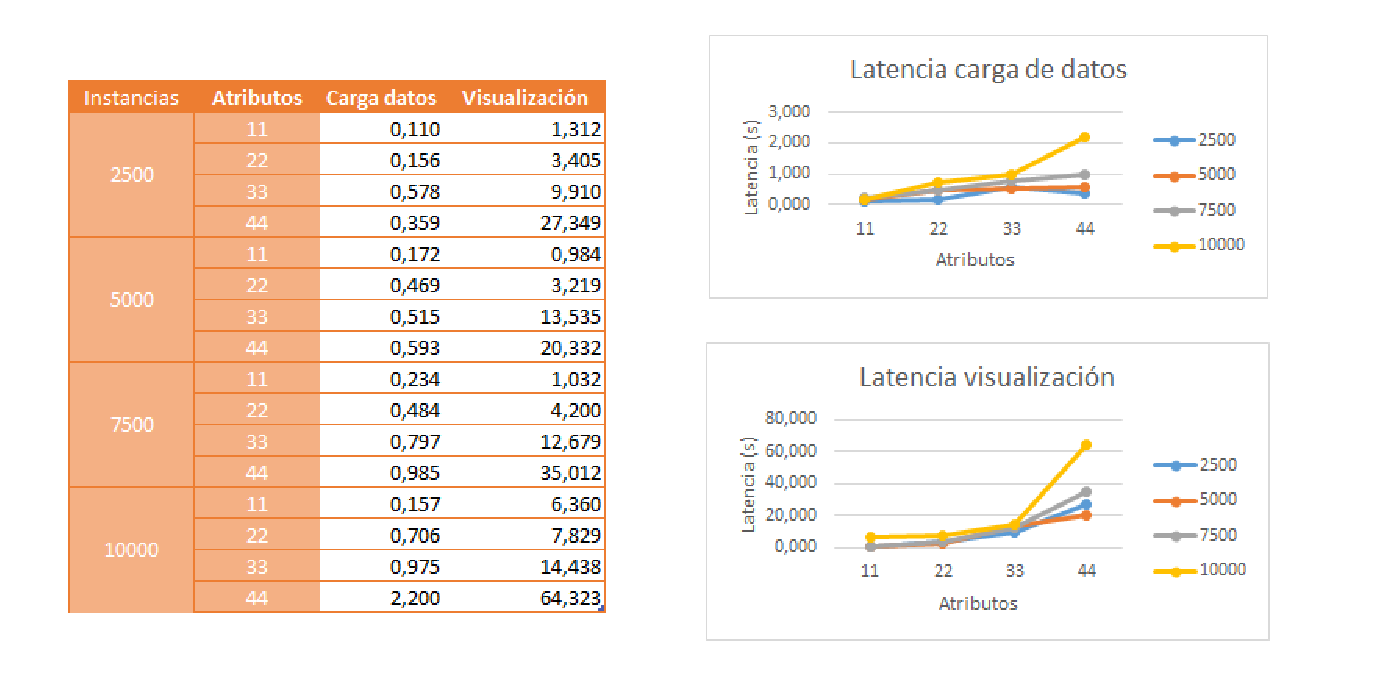
\includegraphics[width=\textwidth,height=\textheight,keepaspectratio]{figuras/eficiencia}
\caption{Comprobación prestacións do RC01}
\label{eficiencia}
\end{figure}
A latencia vólvese crítica no refresco do menú de visualización, e a escalabilidade empeora co aumento do número de atributos. O Modelo sen embargo escala relativamente mellor con respecto a instancias e atributos. Cabe destacar que é ata certo punto razonable que o menú de Visualización escale tan mal, pois sufre os aumentos no número de atributos ao cadrado (a matriz de diagramas ten n*n elementos).
\item[Resultado]
Aceptable.
\end{description}

\subsection{Requisitos de deseño}

\subsubsection*{RD01}
\begin{description}
\item[Título] \hfill
Modularidade no deseño dos filtros
\item[Descrición] \hfill
A aplicación debe facilitar unha interface para a inclusión e uso de filtros personalizados por parte de calquera desenvolvedor de software que a implemente dentro do proxecto.
\item[Importancia] \hfill
Esencial
\item[Tipo de proba] \hfill
Avaliación heurística
\item[Descrición]
O diagrama de deseño exposto neste documento da fe de que se cumpleu este requisito. De todos xeitos pódese probar a nivel de implementación importando un filtro dende JAR.
\item[Resultado]
Correcto.
\end{description}

\subsection{Requisitos non funcionais}

\subsubsection*{RNF01}
\begin{description}
\item[Título] \hfill
Formatos de arquivo admitidos ao importar e exportar arquivos
\item[Descrición] \hfill
A aplicación debe estar preparada para importar e exportar arquivos en distintos formatos, como son o CSV e ARFF.
\item[Importancia] \hfill
Esencial
\item[Tipo de proba] \hfill
Test implementado en JUnit.
\item[Descrición]
Xa foi comprobado no TestRF01\_1 e TestRF01\_2
\item[Resultado]
Correcto.
\end{description}

\subsubsection*{RNF02}
\begin{description}
\item[Título] \hfill
Relación programa-sesión
\item[Descrición] \hfill
Cada instancia do programa debe traballar cunha única sesión (experimento).
\item[Importancia] \hfill
Esencial
\item[Tipo de proba] \hfill
Test implementado en JUnit.
\item[Descrición]
Xa foi comprobado no TestRF0304, xa que ao abrir unha nova sesión perdíase a anterior
\item[Resultado]
Correcto.
\end{description}

\subsubsection*{RNF03}
\begin{description}
\item[Título] \hfill
Implementación en Java
\item[Descrición] \hfill
O software tense que desenvolver na linguaxe de programación Java.
\item[Importancia] \hfill
Esencial
\item[Tipo de proba] \hfill
Avaliación heurística
\item[Descrición]
Podemos comprobalo simplemente accedendo ao código fonte do proxecto.
\item[Resultado]
Correcto.
\end{description}

\subsubsection*{RNF04}
\begin{description}
\item[Título] \hfill
Representación matricial dos diagramas de dispersión
\item[Descrición] \hfill
Os diagramas de dispersión represéntanse de xeito matricial, facendo que cada parámetro dentro dun eixo sexa enfrontado a cada un dos demais do outro eixo, e en cada punto desa dupla se sitúe o diagrama de dispersión que compara ambos parámetros. Deste xeito, os diagramas de dispersión non son acumulables: se temos un que representa X (abscisas) fronte a Y (ordenadas), non podemos engadir outro que represente X (abscisas) fronte a Y (ordenadas), pois ocuparían ambos a mesma cela dentro da matriz de diagramas de dispersión.
\item[Importancia] \hfill
Esencial
\item[Tipo de proba] \hfill
Test implementado en JUnit.
\item[Descrición]
Xa foi comprobado na avaliación heurística de RF11.
\item[Resultado]
Correcto.
\end{description}

\subsubsection*{RNF05}
\begin{description}
\item[Título] \hfill
Entrega dentro de prazo
\item[Descrición] \hfill
Débese entregar unha versión funcional e documentada antes do día 10 de Xullo de 2015, ás 14:00 horas, pois é o momento no que remata o prazo de entrega.
\item[Importancia] \hfill
Esencial
\end{description}

A matriz de trazabilidade que relacionaría cada requisito cun tipo de proba (heurística ou test en JUnit) é a que se presenta a continuación:

\begin{sidewaysfigure}[ht]
\includegraphics[width=\textwidth,height=\textheight,keepaspectratio]{figuras/trazabilidade}
\caption{Matriz de trazabilidade}
\label{trazabilidade}
\end{sidewaysfigure}

% \cleardoublepage
% \chapter{Exemplos}

\section{Un exemplo de sección}
Esta é {\it letra cursiva}, esta é {\bf letra negrilla}, esta é \underline{letra subrallada}, e esta é {\tt letra curier}. Letra {\tiny tiny}, {\scriptsize scriptsize}, {\small small}, {\large large}, {\Large Large}, {\LARGE LARGE} e moitas más. Exemplo de fórmula: $a=\int_o^\infty f(t)dt$.  E agora unha ecuación aparte:

\begin{equation}
S=\sum_{i=0}^{N-1} a_i^2 .
\label{mi_ecuacion}
\end{equation}

As ecuaciones se poden referenciar: ecuación (\ref{mi_ecuacion}).

\subsection{Un exemplo de subsección}
O texto vai aquí.
\subsection{Otro exemplo de subsección}
O texto vai aquí.
\subsubsection{Un exemplo de subsubsección}
O texto vai aquí.
\subsubsection{Un exemplo de subsubsección}
O texto vai aquí.
\subsubsection{Un exemplo de subsubsección}
O texto vai aquí.
\section{Exemplos de figuras e cadros}

A figura número \ref{enlace1}.

O cadro (taboa) número \ref{enlace2}.

\begin{figure}
\centerline{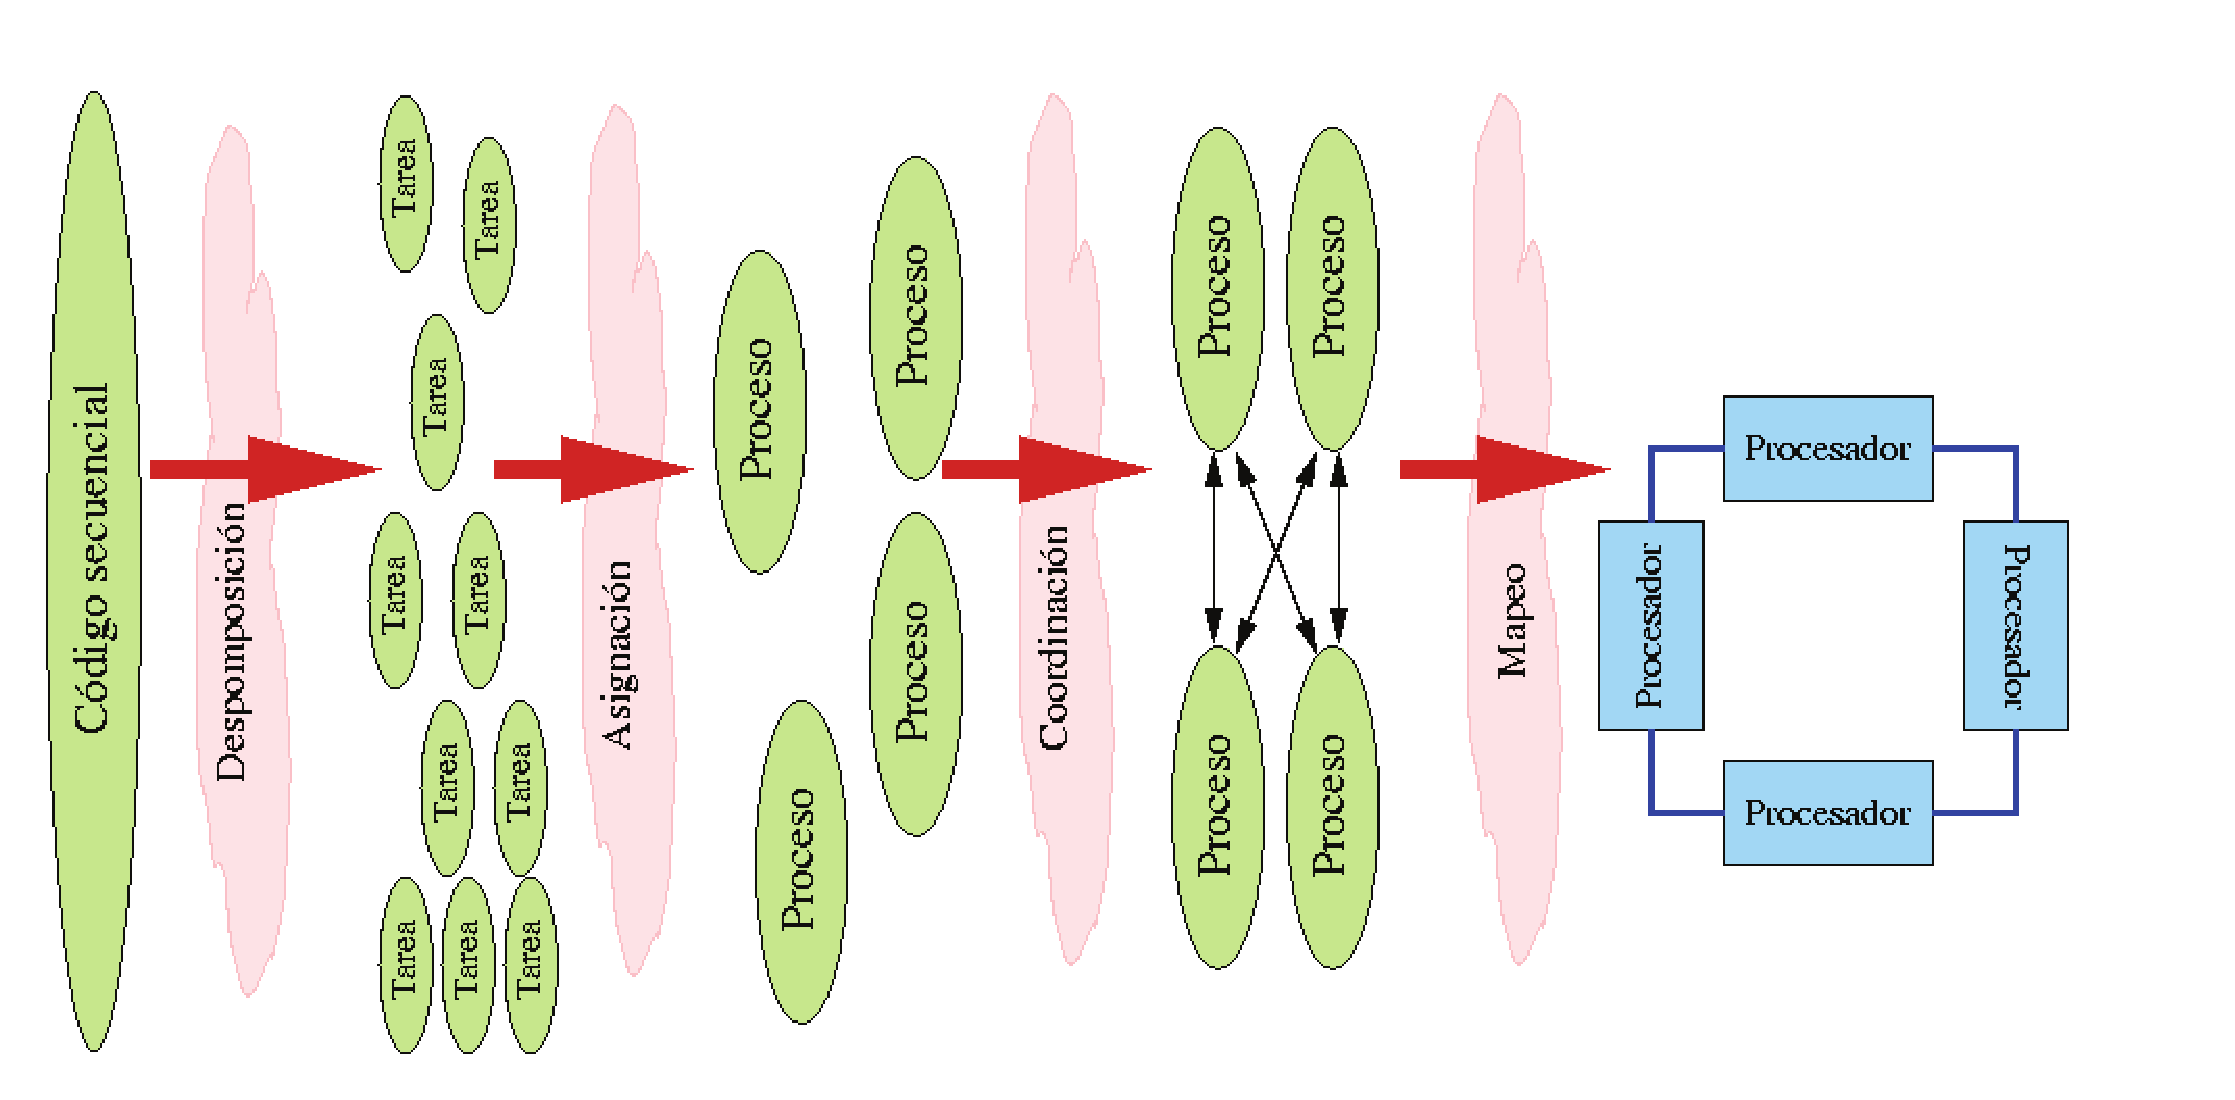
\includegraphics[width=15cm]{figuras/figura01.eps}}
\caption{Esta é a figura de tal e cal.}
\label{enlace1}
\end{figure}

\begin{table}
\begin{center}
\begin{tabular}{|l||r|c|} \hline
Izquierda & Derecha & Centrado  \\ \hline\hline
ll & r & cccc \\ \hline
llll & rrr & c \\ \hline
\end{tabular}
\caption{Esta é a táboa de tal e cal.}
\label{enlace2}
\end{center}
\end{table}

\section{Exemplos de referencias á bibliografía}
Este é un exemplo de referencia a un documento descargado da web \cite{cuda}. E este é un exemplo de referencia a unha páxina da wikipedia \cite{cdma}. Agora un libro \cite{gonzalez} e agora unha referencia a un artigo dunha revista \cite{patricia}. Tamén se poden pór varias referencias á vez \cite{cuda,gonzalez}.

\section{Exemplos de enumeracións}

Con puntos:

\begin{itemize}
\item Un.
\item Dous.
\item Tres.
\end{itemize}

Con números:

\begin{enumerate}
\item Catro.
\item Cinco.
\item Seis.
\end{enumerate}

Exemplo de texto verbatim:

\begin{verbatim}
O texto        verbatim 
     se visualiza tal
            como se escribe
\end{verbatim}

Exemplo de código C:

\lstset{language=C}

\begin{lstlisting}
#include <math.h>
main()
{  int i, j, a[10];
   for(i=0;i<=10;i++) a[i]=i; // comentario 1
   if(a[1]==0) j=1; /* comentario 2 */
   else j=2;
}
\end{lstlisting}

Exemplo de código Java:

\lstset{language=java}

\begin{lstlisting}
class HelloWorldApp {
    public static void main(String[] args) {
        System.out.println("Hello World!"); // Display the string.
    }
}
\end{lstlisting}



%
% Engadir os capitulos que fagan falta
%
\cleardoublepage
\chapter{Conclusións e posibles ampliacións}

Conclusións e posibles ampliacións


% Aquí empezan os apéndices
\appendix
\cleardoublepage
\chapter{Manuais técnicos}

Manuais técnicos: en función do tipo de Traballo e metodoloxía empregada, o contido poderase dividir en varios documentos. En todo caso, neles incluirase toda a información precisa para aquelas persoas que se vaian a encargar do desenvolvemento e/ou modificación do Sistema (por exemplo código fonte, recursos necesarios, operacións necesarias para modificacións e probas, posibles problemas, etc.). O código fonte poderase entregar en soporte informático en formatos PDF ou postscript.

\cleardoublepage
\chapter{Manuais de usuario}

Neste manual sinalaremos onde atopar as distintas funcionalidades que prove JDataMotion. Abordarémolas seguindo unha suxerencia de execución, de acordo á traza de uso máis común que quizais poda recibir a aplicación.

\section{Requisitos do sistema}

Para a executar a aplicación JDataMotion abonda con ter instalada unha versión da máquina virtual de Java igual ou superior a 1.8, a cal podemos descargar dende o sitio web oficial \cite{java}.

Aconséllase empregar a ferramenta nun sistema con 2GB ou máis de memoria RAM.

\section{Instalación e arranque}

O primeiro paso é instalar o software no noso equipo. Para isto podemos emprazar a carpeta JDataMotion da aplicación no directorio que prefiramos (por exemplo, a carpeta persoal). A carpeta da aplicación está contida dentro da carpeta do proxecto, coa que comparte nome. Sinalámola para despexar dúbidas na figura \ref{carpetaAplicacion}

\begin{figure}
\centering

\includegraphics[width=\textwidth,height=\textheight,keepaspectratio]{figuras/carpetaAplicacion}
\caption{Carpeta da aplicación JDataMotinon (seleccionada)}
\label{carpetaAplicacion}
\end{figure}

Unha vez que escollemos o emprazamento para a aplicación, accedemos a ela e seguimos estes pasos en función do noso sistema operativo:

\begin{itemize}
\item Para sistemas baseados en Windows, buscamos o ficheiro ``run.bat''. Podemos crear un acceso directo a este arquivo en calquera outro lugar, pero non copialo ou movelo a outro directorio.
\item Para sistemas baseados en Linux, abrimos primeiramente un terminal e desprazámonos ata o directorio da aplicación. Introducimos o comando ``sudo chmod +x run.sh'' e introducimos o contrasinal de administrador. Podemos crear un lanzador cara este arquivo en calquera outro lugar, pero non copialo ou movelo a outro directorio. Executamos o arquivo con ./run.sh
\end{itemize}

En calquera dos dous casos, apareceranos unha ventá parecida á da figura \ref{inicial}.

\begin{figure}
\centering
\includegraphics[width=\textwidth,height=\textheight,keepaspectratio]{figuras/inicial}
\caption{Ventá de JDataMotion}
\label{inicial}
\end{figure}

\section{Utilización}

Para comezar a traballar temos dúas vías. A primeira é crear un novo experimento importando un ficheiro en formato .csv ou .arff. Para isto iríamos a Ficheiro \textgreater{} Importar ficheiro. A continuación buscaríamos no explorador un ficheiro cunha extensión válida (ver figura \ref{importarFicheiro}).

\begin{figure}
\centering
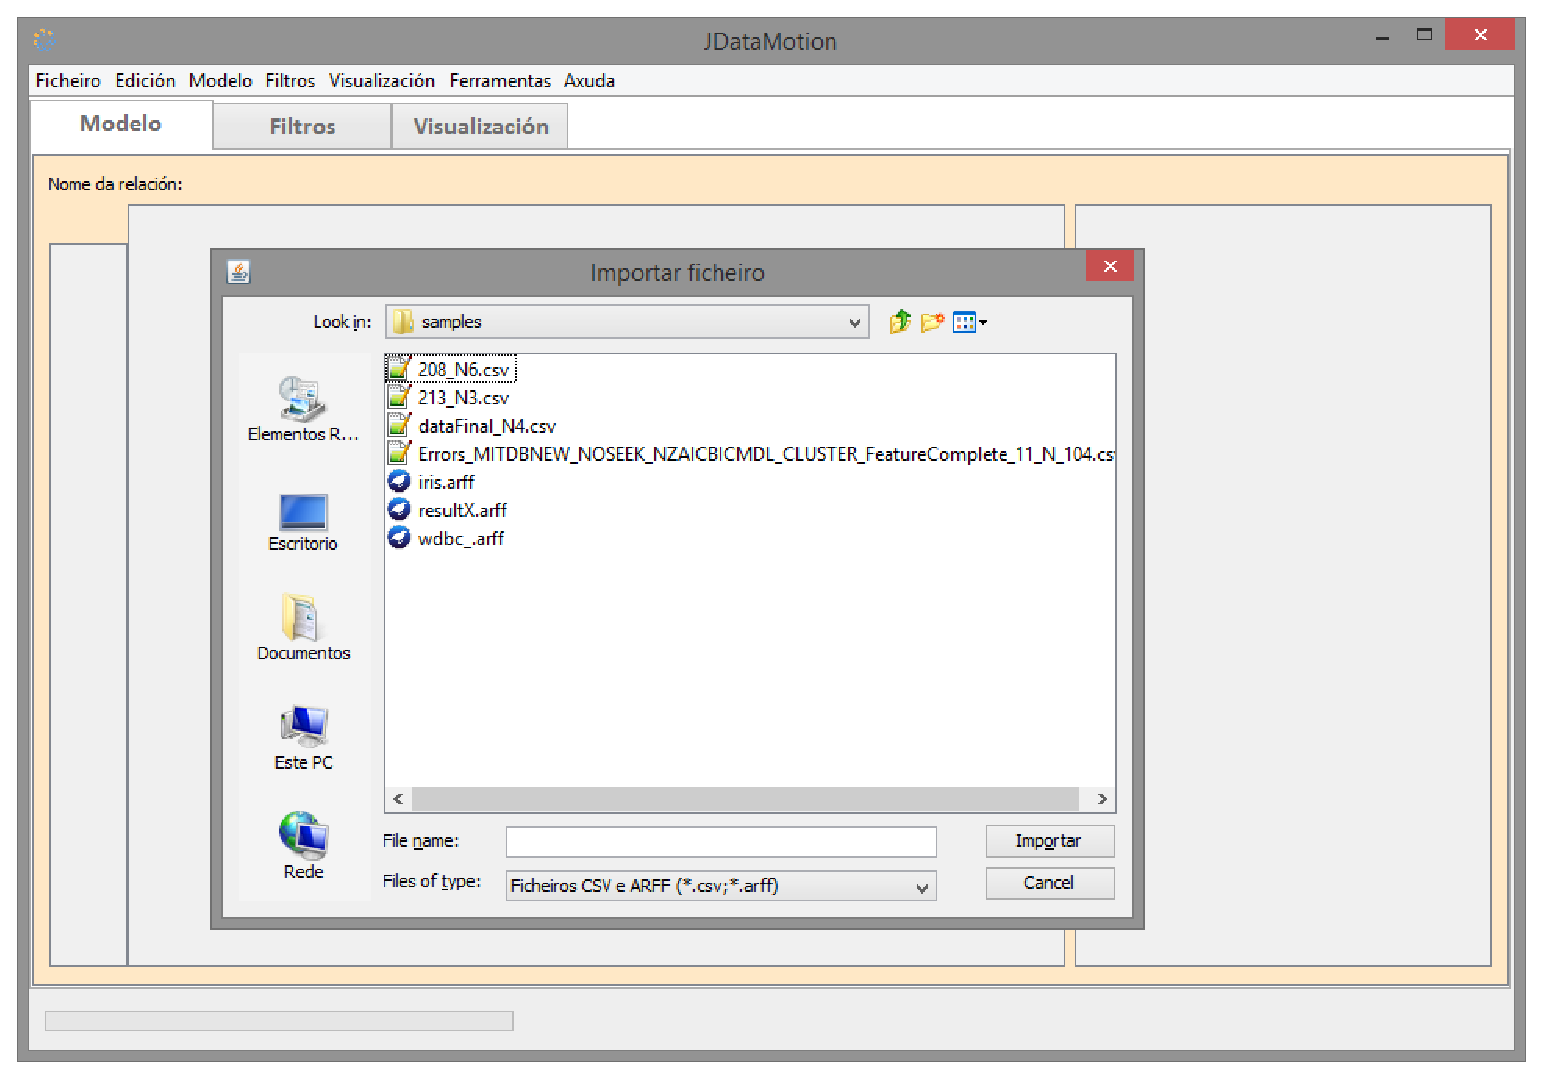
\includegraphics[width=\textwidth,height=\textheight,keepaspectratio]{figuras/importarFicheiro}
\caption{Importación dun ficheiro}
\label{importarFicheiro}
\end{figure}

A outra forma de comezar a traballar é abrir unha sesión gardada previamente. Para isto iríamos a Ficheiro \textgreater{} Abrir sesión. A continuación buscaríamos no explorador un ficheiro coa extensión .jdms (ver figura \ref{abrirSesion}).

\begin{figure}
\centering
\includegraphics[width=\textwidth,height=\textheight,keepaspectratio]{figuras/abrirSesion}
\caption{Abrir unha sesión}
\label{abrirSesion}
\end{figure}

\subsection{Modelo}

O menú Modelo encherase representando os atributos nas cabeceiras da táboa, e os datos como filas da mesma (ver figura \ref{manualModelo}).

\begin{figure}
\centering
\includegraphics[width=\textwidth,height=\textheight,keepaspectratio]{figuras/manualModelo}
\caption{Modelo con datos}
\label{manualModelo}
\end{figure}

Se pinchamos nalgunha das cabeceiras da táboa veremos no panel da dereita un resumo dos datos que contén, ademais dun histograma cos valores que toma. Podemos facer que este histograma agrupe as barras segundo un atributo nominal (tamén chamado atributo de clase). Para isto deberemos especificar cal queremos usar, dirixíndonos ao menú Visualización \textgreater{} Establecer atributo nominal representado, e seleccionando o atributo que prefiramos. Se non aparece o que se desexa usar, teremos que cambiarlle o tipo a ``nominal'' para que estea dispoñible. O resultado será algo parecido ao da figura \ref{histogramaNominal}.

\begin{figure}
\centering
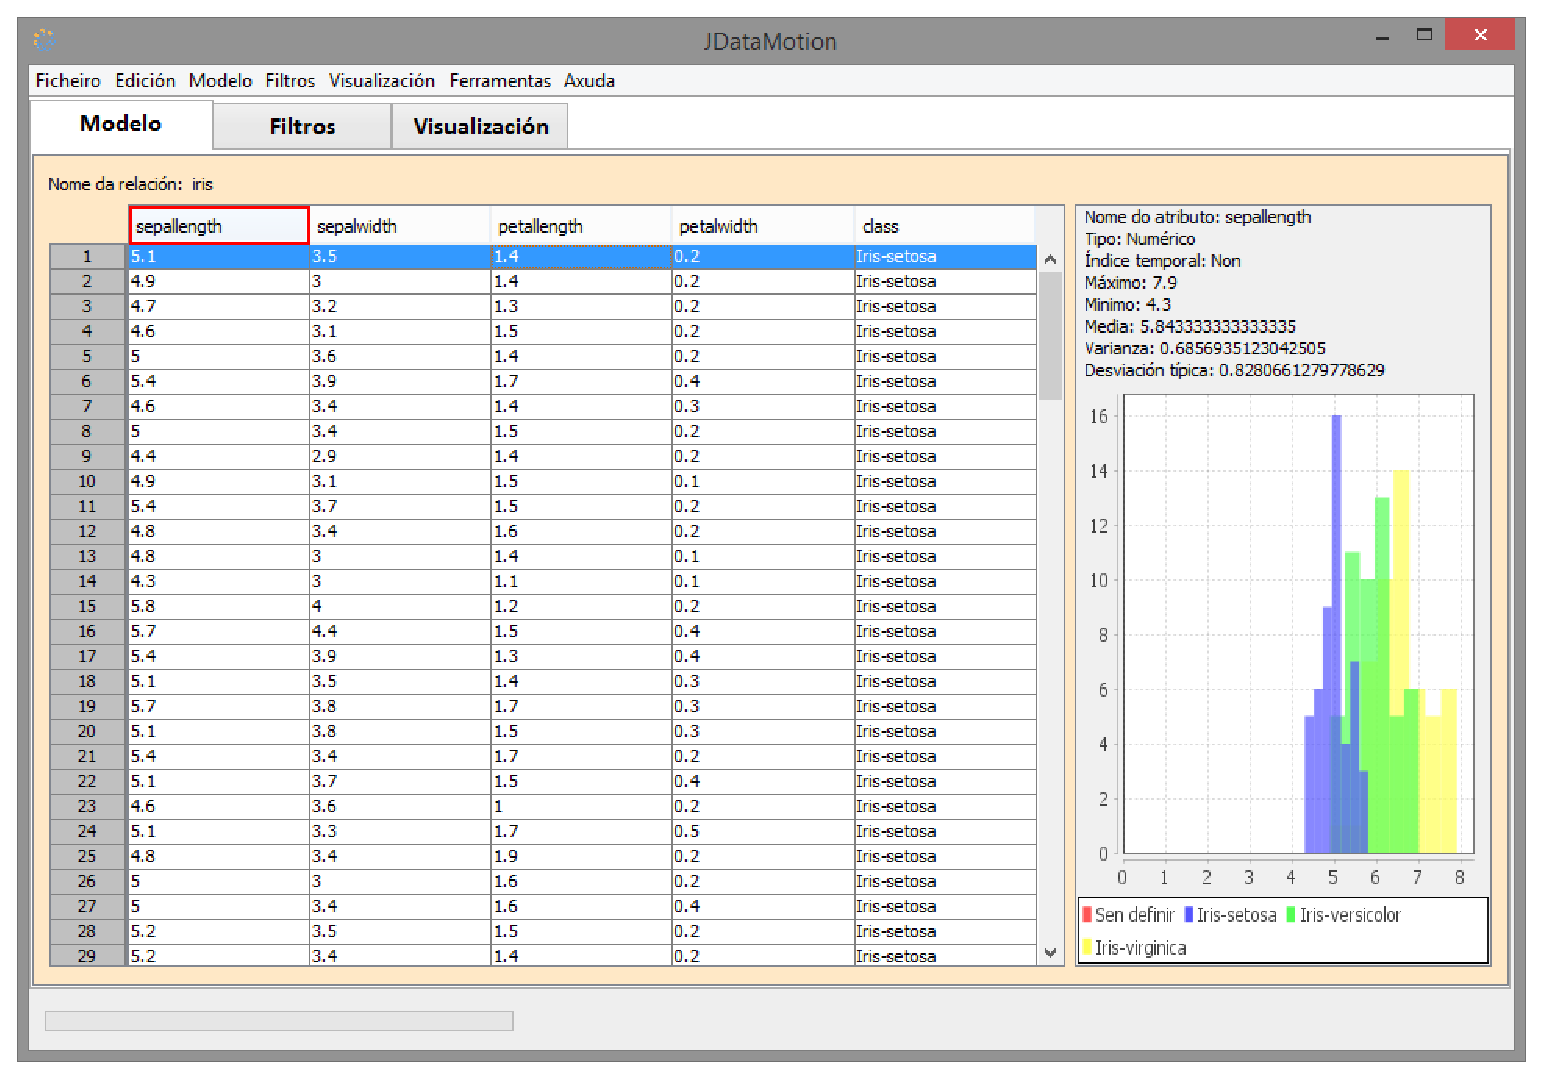
\includegraphics[width=\textwidth,height=\textheight,keepaspectratio]{figuras/histogramaNominal}
\caption{Histograma que usa un atributo nominal}
\label{histogramaNominal}
\end{figure}

Para mudar o tipo dun atributo debemos premer na súa cabeceira co botón secundario. Sairá un menú emerxente con varios ítems (ver figura \ref{menuAtributo}), iremos a Tipo e a continuación seleccionaremos o tipo ao que queremos que se converta o atributo e máis os seus datos. A conversión deixará campos baleiros onde non sexa capaz de realizar a conversión (por exemplo, se pasamos a numérico un atributo que ten un texto nunha celda).

\begin{figure}
\centering
\includegraphics[width=\textwidth,height=\textheight,keepaspectratio]{figuras/menuAtributo}
\caption{Menú emerxente dos atributos}
\label{menuAtributo}
\end{figure}

No menú emerxente dos atributos tamén temos a opción Agochar columna, que a quitará do menú sen eliminar os seus elementos. Para restablecer as columnas ocultadas, iremos a Modelo \textgreater{} Amosar todas as columnas. A última posibilidade deste menú contextual permítenos asignar o índice temporal ao atributo no que se premeu. O atributo debe ser de tipo numérico, ou de tipo String contendo valores nun formato de tempo ([[HH:]mm:]ss). Establecendo o índice temporal poderemos facer que as reproducións posteriores sigan a orde do atributo que é o índice temporal.

Pulsando dúas veces unha cela da táboa podemos editar o seu valor. Se o atributo é de tipo nominal, despregarásenos unha lista dos posibles valores que pode tomar. Se o novo dato que inserimos nesa cela non é compatible co atributo ao que pertence notificarásenos o erro.

Podemos engadir ou eliminar tanto filas (instancias) coma columnas (atributos) á táboa do Modelo.

Para engadir filas iremos a Modelo \textgreater{} Engadir instancia. A nova instancia figura baleira ao final da táboa (ver figura \ref{engadirInstancia}). Podémoslle asignar valores premendo dúas veces nas celas que a compoñen.

\begin{figure}
\centering
\includegraphics[width=\textwidth,height=\textheight,keepaspectratio]{figuras/engadirInstancia}
\caption{Resultado de engadir instancia}
\label{engadirInstancia}
\end{figure}

Se desexamos eliminar un conxunto de filas, primeiro teremos que seleccionalas na táboa. Pódense seleccionar varias mantendo pulsada a tecla Control, ou pulsar a tecla Mayus e seleccionar dúas filas, de xeito que tamén queden seleccionadas as filas que as separan. Unha vez teñamos a selección feita, iremos a Modelo \textgreater{} Eliminar instancias, para descartalas.

Os atributos engádense por medio de Modelo \textgreater{} Engadir atributo. Ao facelo, a táboa contará cun atributo máis ao final, chamado ``novoAtributo''. Este atributo novo é por defecto de tipo String. Esto podémolo apreciar na figura \ref{engadirAtributo}.

\begin{figure}
\centering
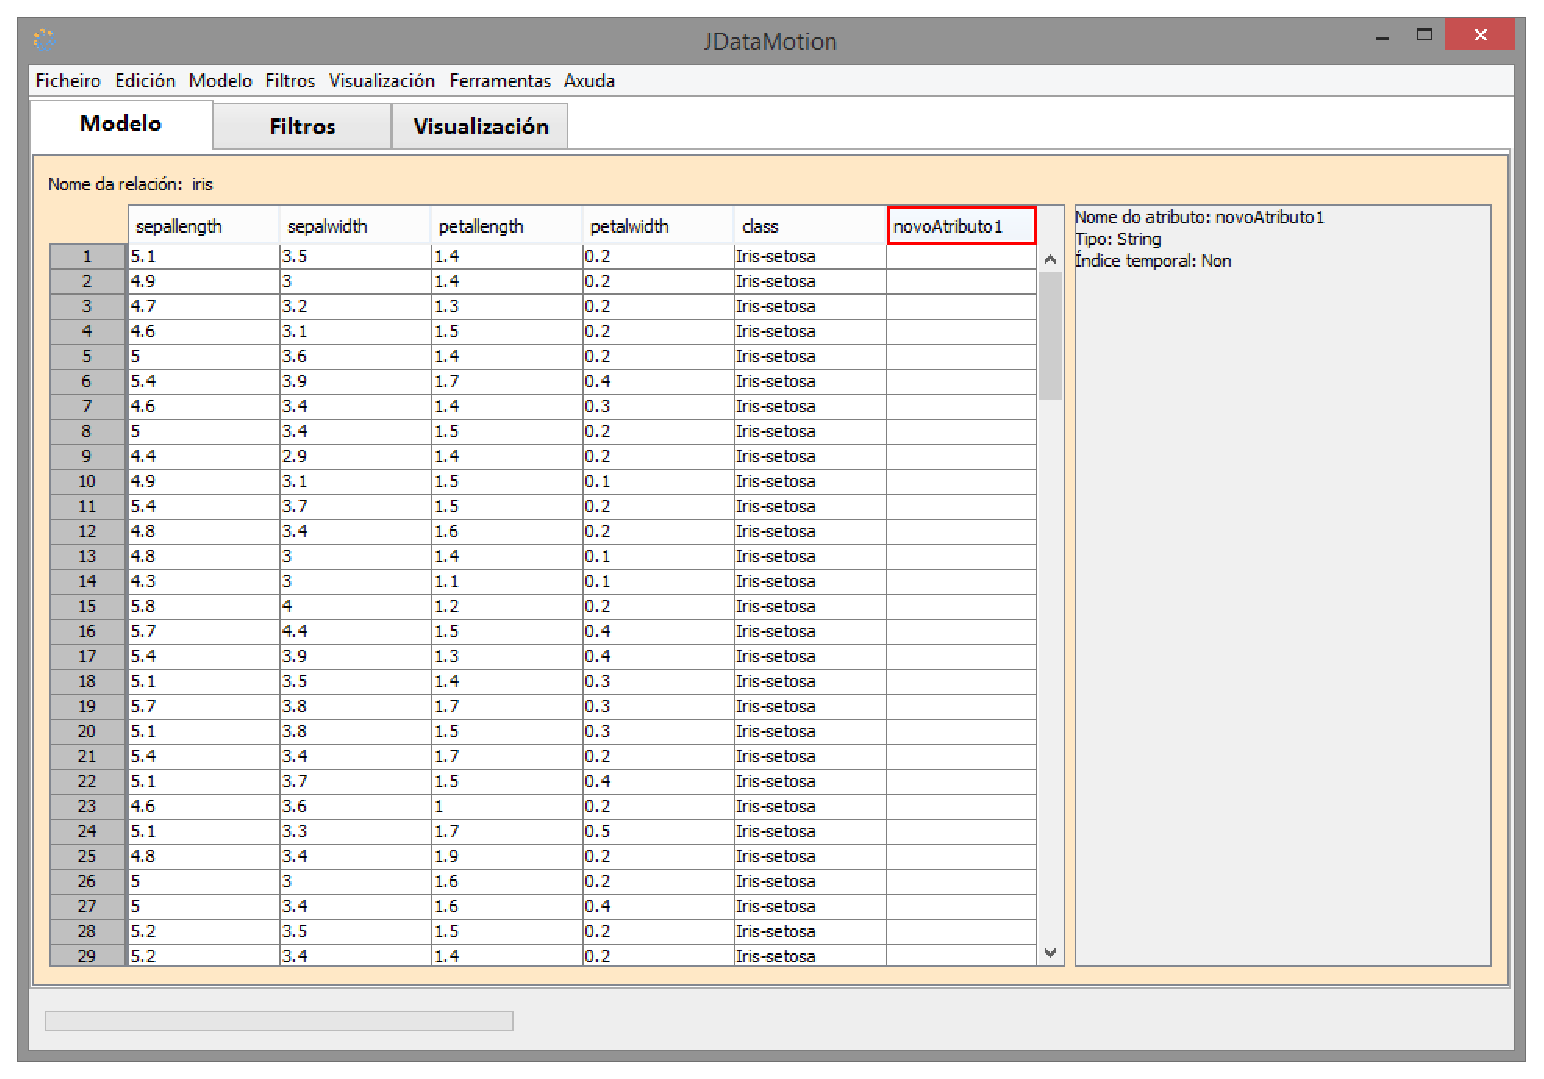
\includegraphics[width=\textwidth,height=\textheight,keepaspectratio]{figuras/engadirAtributo}
\caption{Resultado de engadir atributo}
\label{engadirAtributo}
\end{figure}

Podemos eliminar atributos seleccionándoos e, a continuación, indo a Modelo \textgreater{} Eliminar atributo.

Tamén podemos mudar o nome dun atributo seleccionándoo e indo a Modelo \textgreater{} Renomear atributo. Inserimos o novo nome do atributo e aceptamos. Non se deben duplicar nomes de atributos, se o novo nome do atributo xa existe, o sistema avisaranos do erro.

Por último, podemos cambiarlle o nome á relación de datos coa que estamos traballando con Modelo \textgreater{} Mudar nome da relación.

Para descartar todos os cambios e recargar o ficheiro orixinal podemos usar a función Modelo \textgreater{} Restaurar.

\subsection{Filtros}

Unha vez lle demos formato ou completemos os datos do Modelo, podemos avanzar cara a segunda lapela da aplicación, que amosará o menú de Filtros, tal e como se amosa na figura \ref{manualFiltros}

\begin{figure}
\centering
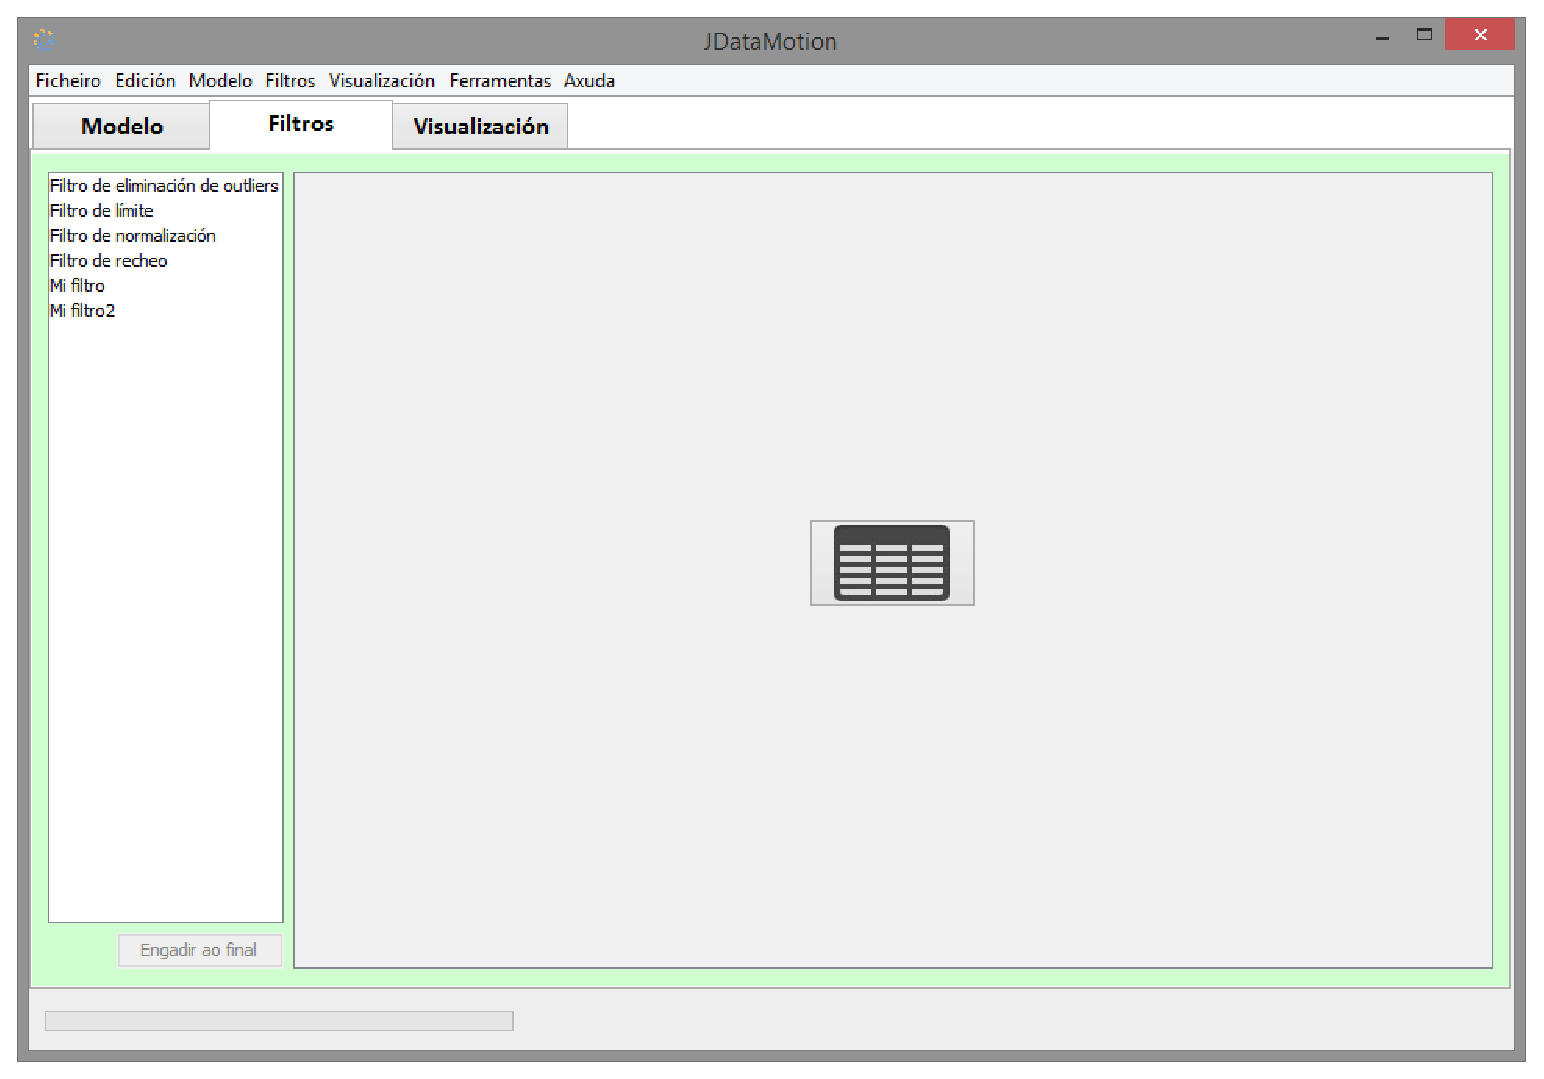
\includegraphics[width=\textwidth,height=\textheight,keepaspectratio]{figuras/manualFiltros}
\caption{Menú Filtros}
\label{manualFiltros}
\end{figure}

Neste menú poderemos seleccionar filtros da lista situada á esquerda, e premer en ``Engadir ao final'' para situar o filtro na secuencia. A medida que engadamos filtros esta secuencia irá aumentando (ver figura \ref{secuenciaFiltros}).

\begin{figure}
\centering
\includegraphics[width=\textwidth,height=\textheight,keepaspectratio]{figuras/secuenciaFiltros}
\caption{Secuencia de filtros}
\label{secuenciaFiltros}
\end{figure}

Dentro do panel que ilustra a secuencia temos varios ítems. Por unha parte, a primeira icona empezando pola esquerda pódese premer, para ampliar nunha ventá aparte o modelo de datos do que se parte antes de aplicar ningún filtro.

Os embudes verdes representan os filtros engadidos. Se saen cun signo de admiración en amarelo, significa que algún parámetro do filtro está sen definir, e polo tanto o filtro non se está aplicando realmente.

Para configurar un filtro temos que premer a primeira das iconas que ten baixo a súa representación (uns engrenaxes negros). Aparecerá unha ventá para inserir os valores que necesita o filtro. Unha vez os insertemos todos, o icono de ``filtro sen configurar'' desaparecerá (ver figura \ref{filtrosConfigurados}).

\begin{figure}
\centering
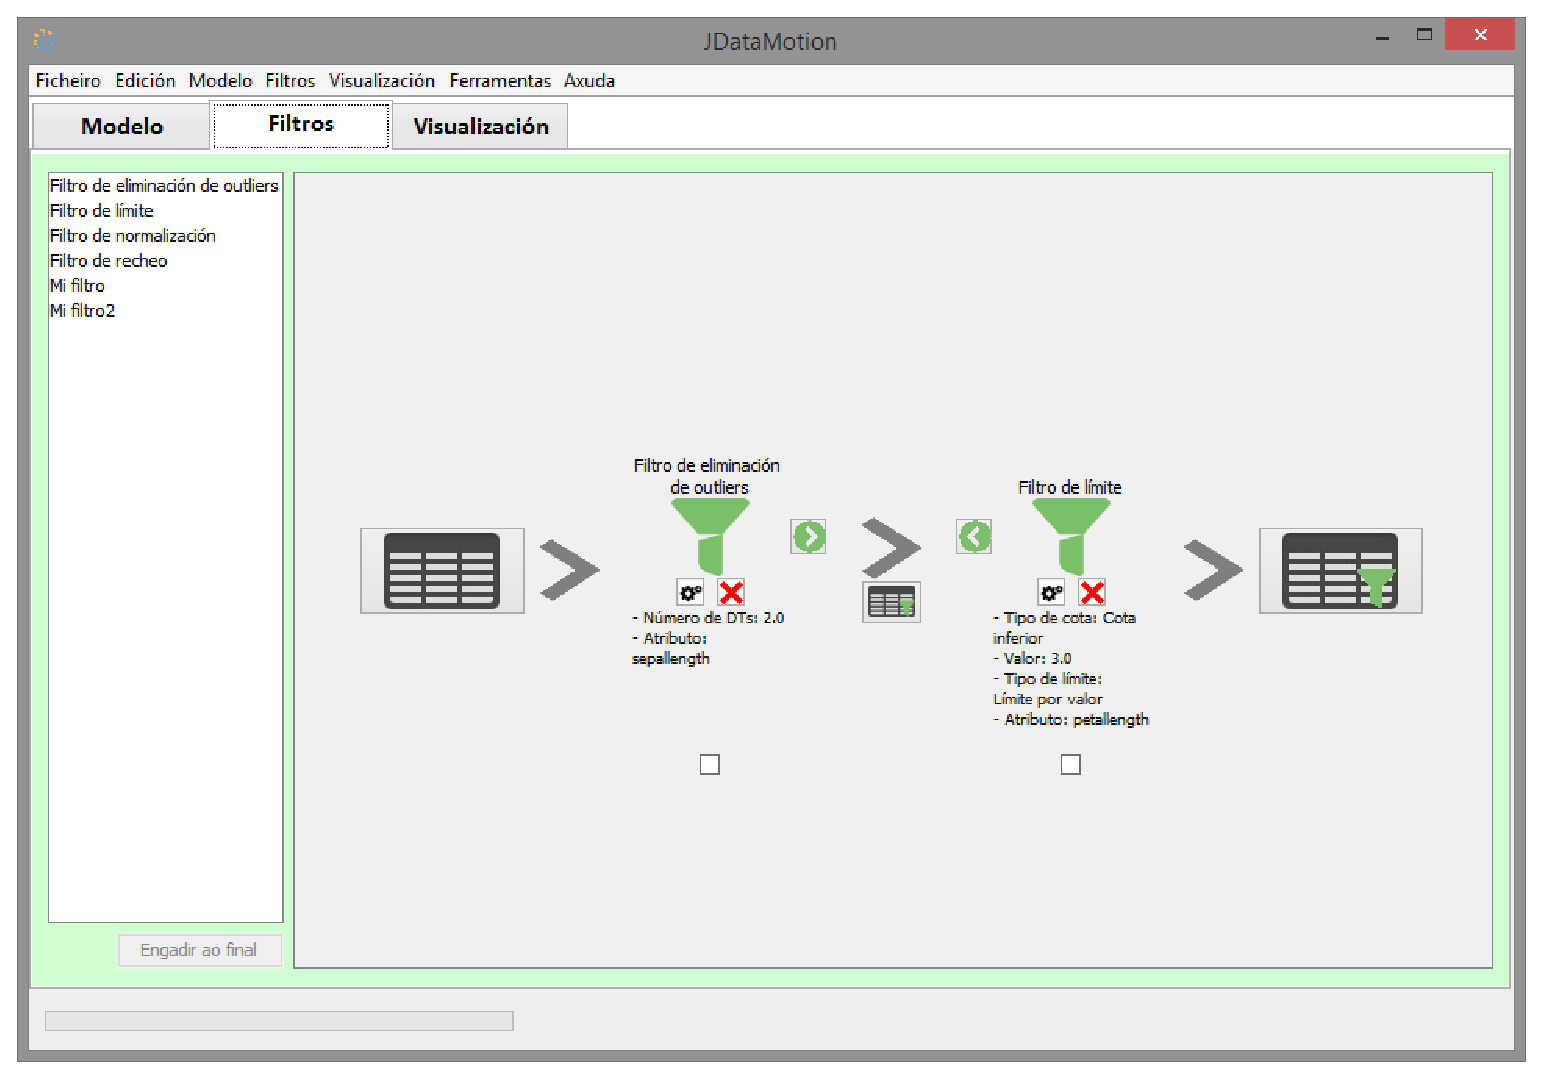
\includegraphics[width=\textwidth,height=\textheight,keepaspectratio]{figuras/filtrosConfigurados}
\caption{Filtros configurados}
\label{filtrosConfigurados}
\end{figure}

A icona contigua á de configuración (cunhas aspas vermellas) serve para eliminar o filtro da secuencia, anulando os seus efectos.

A frecha verde que cada filtro pode ter aos seus lados permite mover o filtro na secuencia, alterando a orde de aplicación.

Entre cada dous filtros consecutivos temos unha icona de táboa de menor tamaño. Premer nela amósanos como se atopa o modelo ata ese punto, tras aplicarse todos os filtros á esquerda pero ningún da dereita aínda. Trátase da representación dun modelo parcial.

Por último, a icona á dereita da secuencia (unha táboa cun embude) mostra o modelo final, tras a aplicación de toda a secuencia de filtros. Este modelo final será co que se vaia a traballar no último menú da aplicación.

Podemos seleccionar filtros utilizando o checkbox ou cadro seleccionable que teñen debaixo. Seleccionar filtros permitiranos utilizar a opción Filtros \textgreater{} Exportar filtros seleccionados. Ao facelo, pedirase un directorio e un nome de arquivo no que se almacenarán os filtros marcados baixo un arquivo de extensión .jdmf.

Eses filtros poden ser logo recuperados en calquera sesión. Se os volvemos a importar, engadiranse ao final da secuencia, tal e como podemos observar na figura \ref{filtrosRecuperados}.

\begin{figure}
\centering
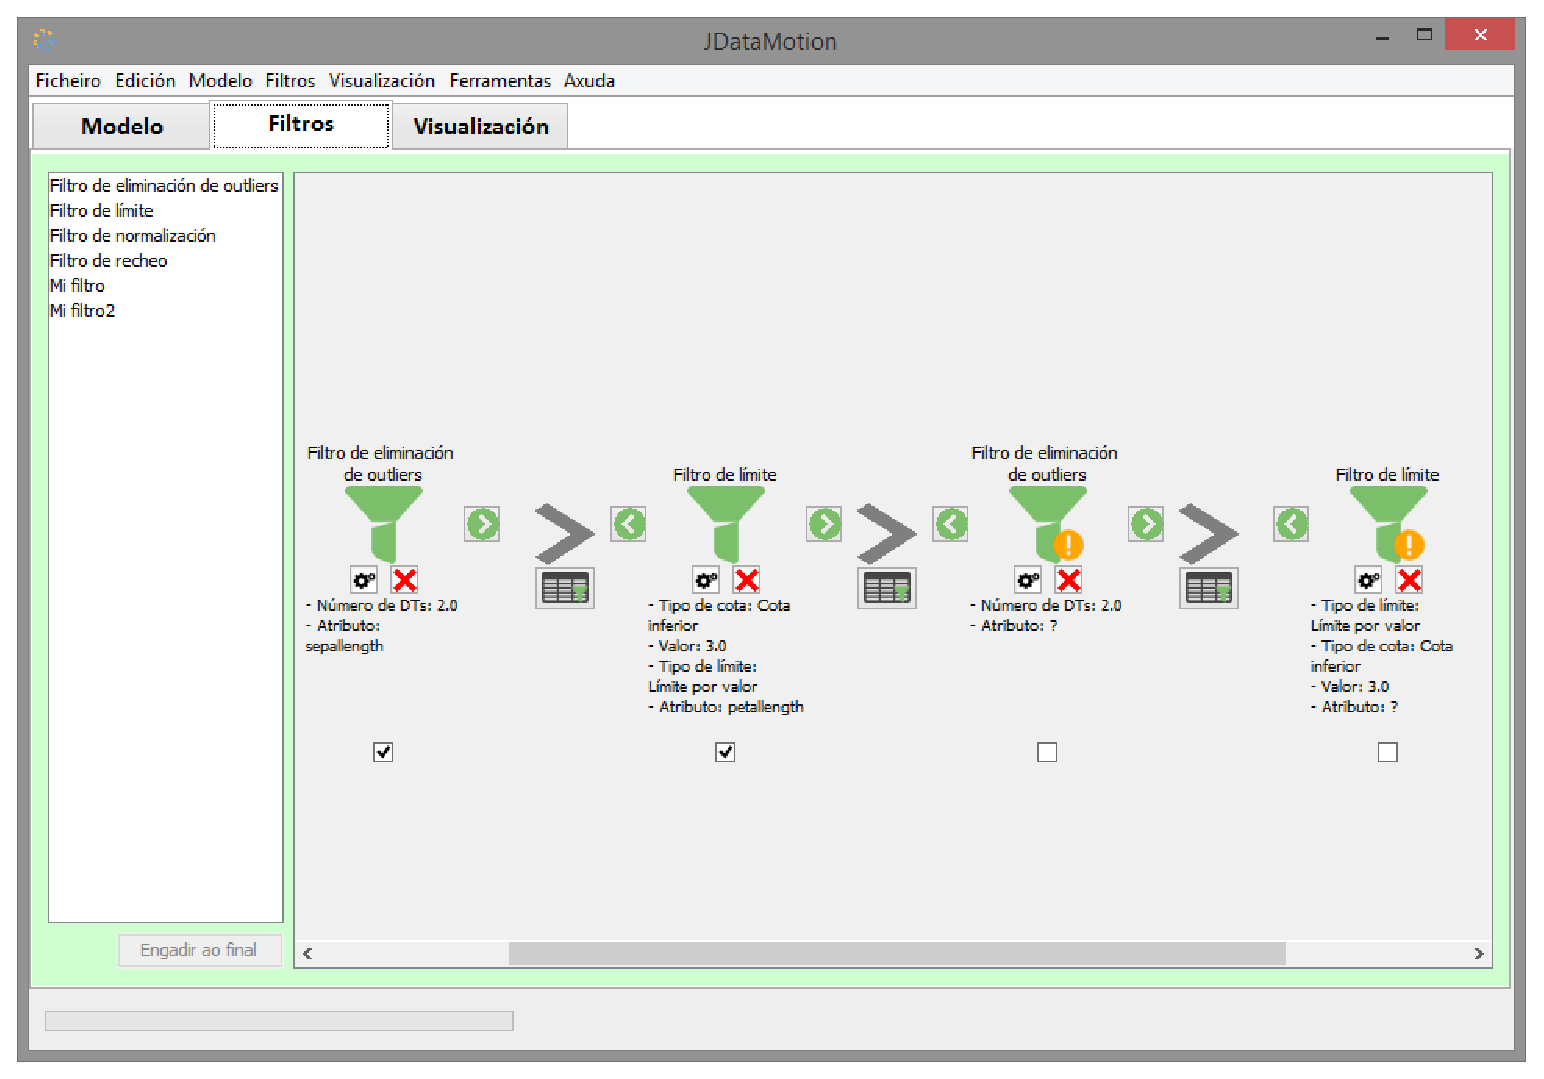
\includegraphics[width=\textwidth,height=\textheight,keepaspectratio]{figuras/filtrosRecuperados}
\caption{Filtros exportados e importados}
\label{filtrosRecuperados}
\end{figure}

Nótese que para preservar a integridade dos filtros entre experimentos distintos, estes perden o atributo sobre o que actúan ao seren importados, co cal temos que volver a configurar este parámetro.

Por último, podemos aumentar a lista de filtros dispoñibles na lista da esquerda importándoos dende unha libraría en formato .jar. Para isto, iremos a Filtros \textgreater{} Importar filtro dende JAR e indicaremos no explorador que ficheiro queremos analizar na procura de filtros. Nótese que un filtro é calquera clase que implemente a interface IFilter que proporciona este proxecto.

\subsection{Visualización}

Chegados a este punto xa temos os datos do ficheiro preprocesados e filtrados, así que agora imos a representalos dinamicamente. Para iso accedemos á última lapela da aplicación, que nos amosará o Menú Visualización, que será parecido ao da figura \ref{manualVisualizacion}.

\begin{figure}
\centering
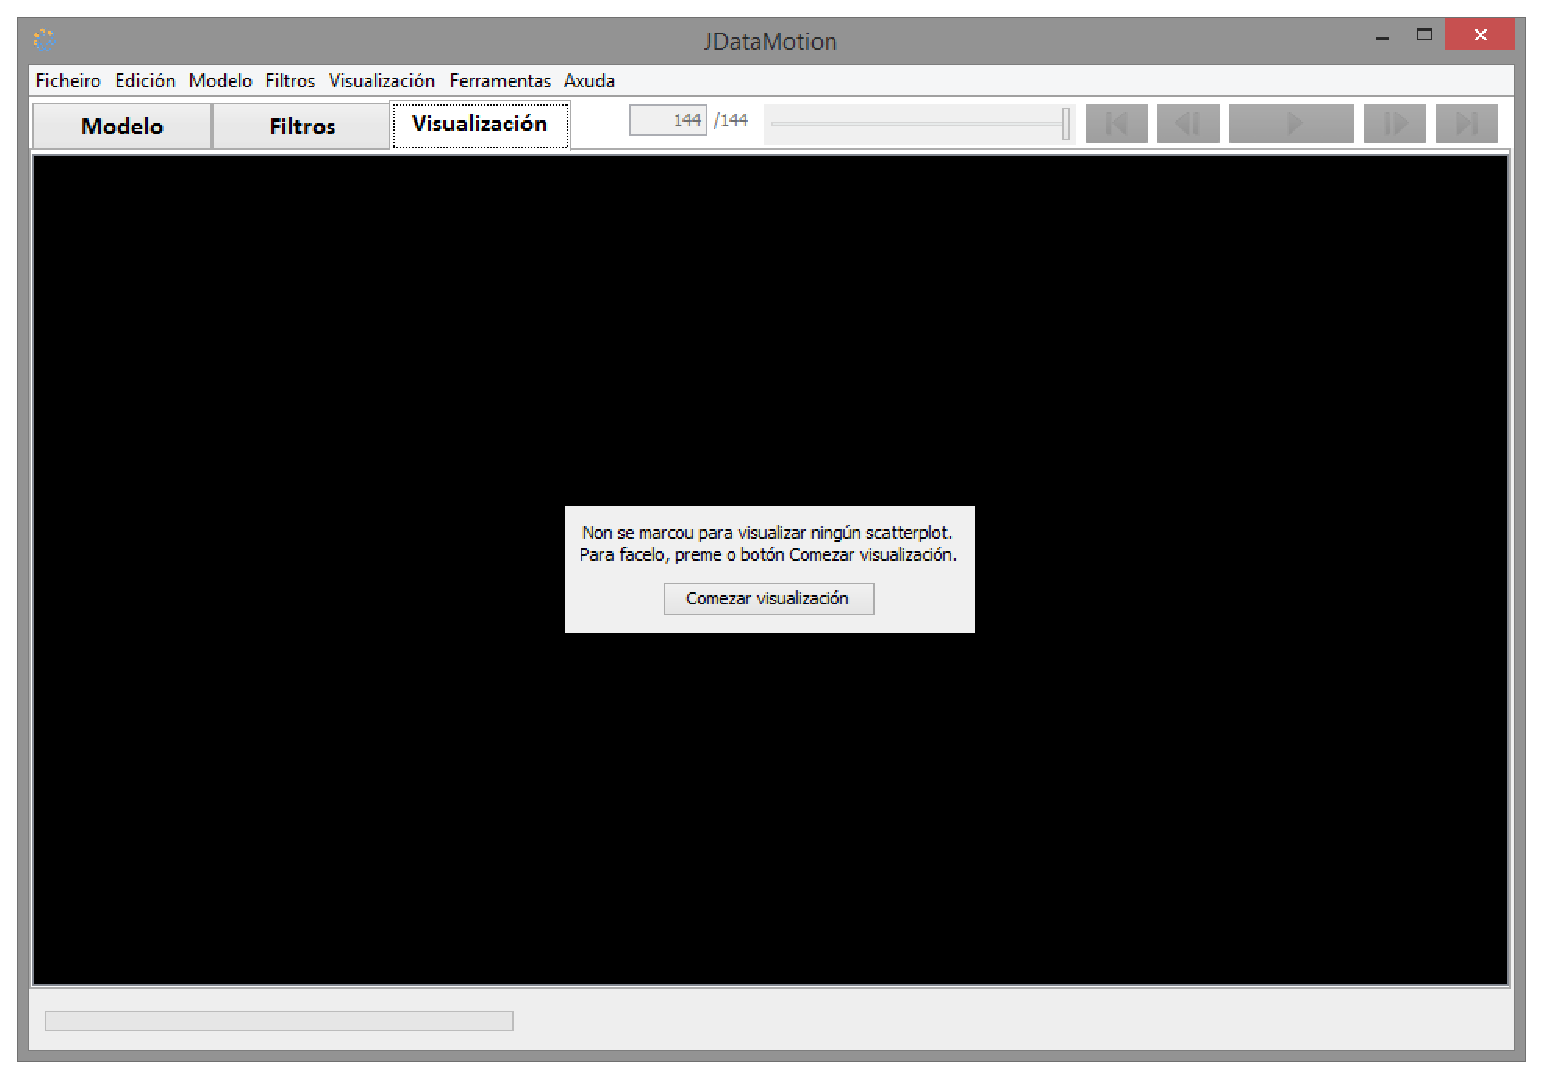
\includegraphics[width=\textwidth,height=\textheight,keepaspectratio]{figuras/manualVisualizacion}
\caption{Menú Visualización}
\label{manualVisualizacion}
\end{figure}

A primeira vez que accedemos a este menú non haberá nada, e suxerirannos engadir algún scatterplot ou diagrama de dispersión por medio do botón ``Comezar visualización''. Premémolo e veremos unha matriz parecida á da figura \ref{matrizVisualizacion}.

\begin{figure}
\centering
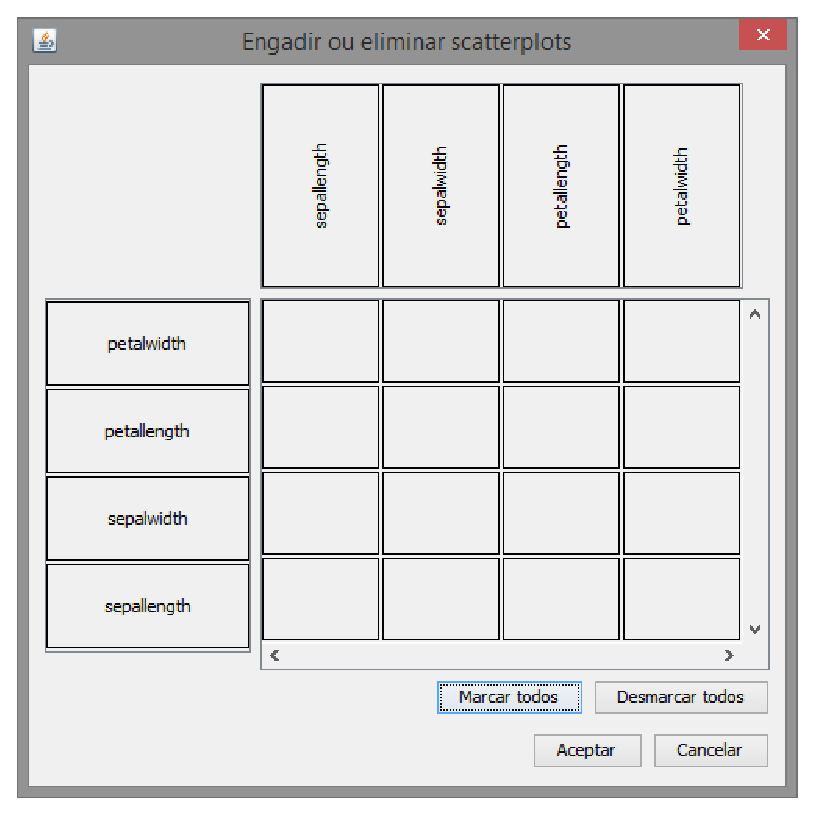
\includegraphics[width=\textwidth,height=\textheight,keepaspectratio]{figuras/matrizVisualizacion}
\caption{Matriz seleccionable de diagramas}
\label{matrizVisualizacion}
\end{figure}

Esta matriz amosa tantas celas como posibles diagramas se poden visualizar. Cada diagrama é a combinación de dous atributos numéricos, un para definir os valores das abscisas (o atributo da columna) e outro para definir os valores das ordenadas (o atributo da fila). Podemos seleccionar e deseleccionar diagramas nesta ventá individualmente (iranse marcando en amarelo as que se desexen visualizar) ou seleccionalas/deseleccionalas todas á vez.

Unha vez fagamos a nosa selección, o menú de Visualización debería encherse con algo semellante ao da figura \ref{matrizChea}.

\begin{figure}
\centering
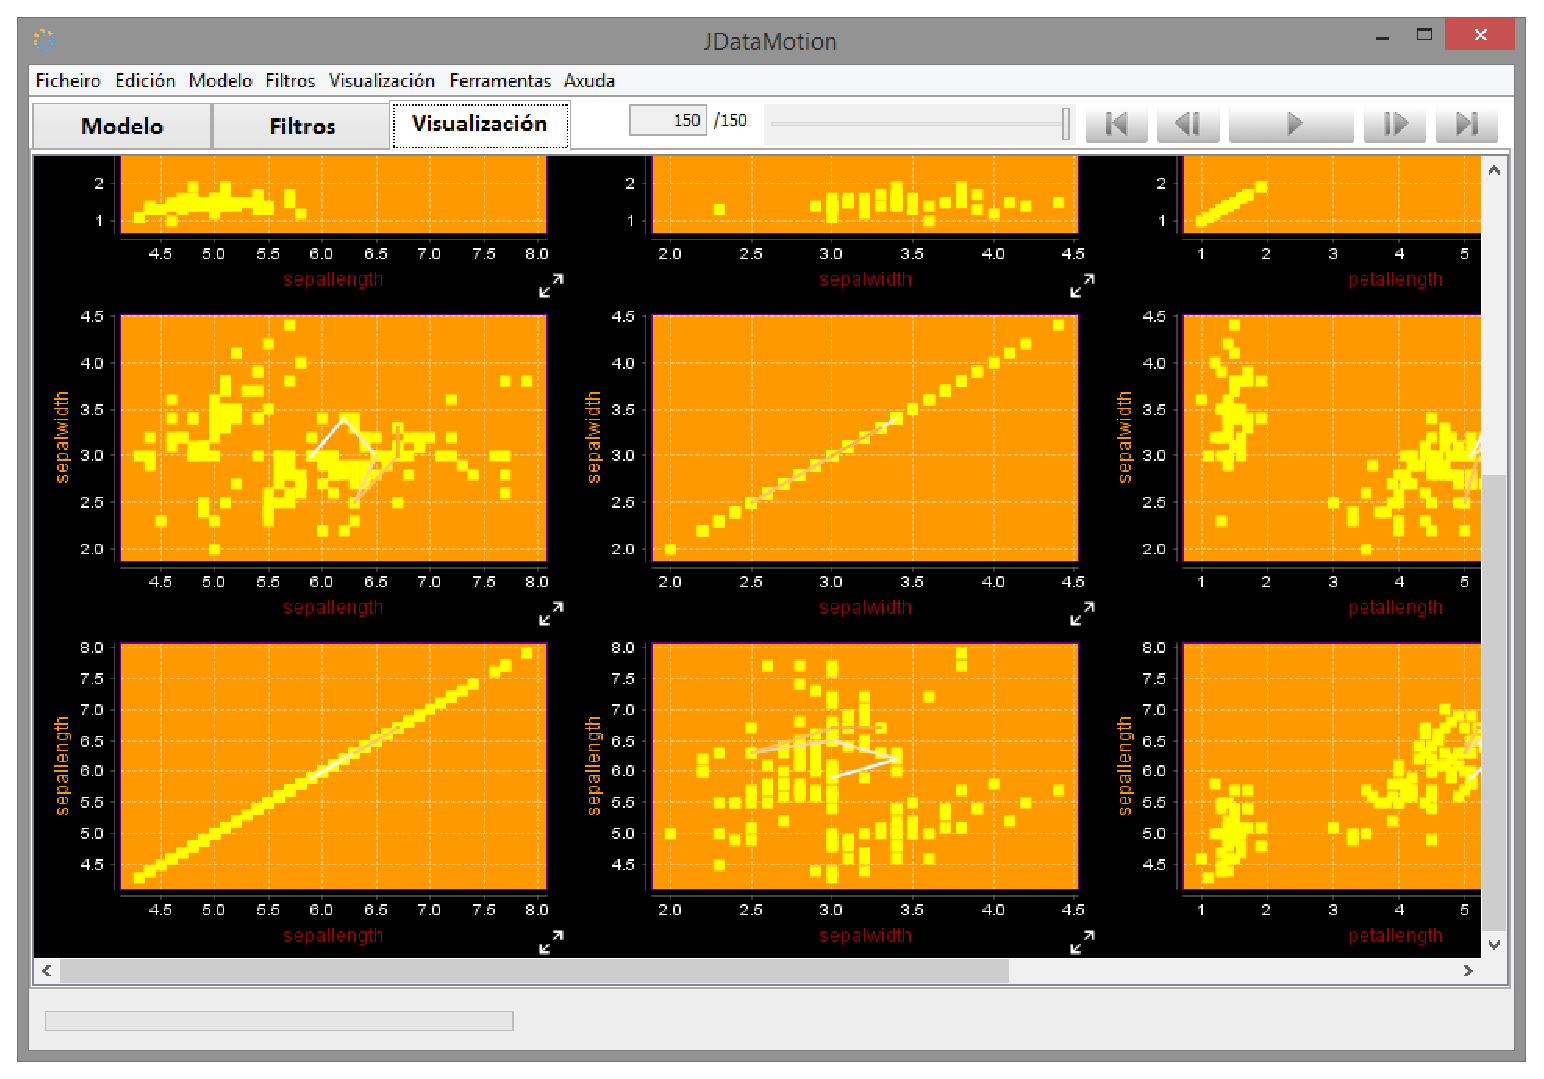
\includegraphics[width=\textwidth,height=\textheight,keepaspectratio]{figuras/matrizChea}
\caption{Matriz de visualización}
\label{matrizChea}
\end{figure}

Todos os diagramas que agora están no Menú de Visualización teñen unha icona con forma de dúas frechas na esquina sueste. Podemos premelos para ampliar un ou varios diagramas nunha ventá aparte.

Se seleccionamos un atributo nominal durante o noso paso polo menú Modelo, ou mesmo se o seleccionamos agora, os diagramas amosarán os puntos agrupados segundo un atributo que será tomado como atributo de clase, tal e como se mostra na figura \ref{diagramasNominais}.

\begin{figure}
\centering
\includegraphics[width=\textwidth,height=\textheight,keepaspectratio]{figuras/diagramasNominais}
\caption{Diagramas con atributo de clase}
\label{diagramasNominais}
\end{figure}

Para volver á ventá para seleccionar que diagramas queremos ver, podemos acceder por medio de Visualización \textgreater{} Engadir ou eliminar scatterplots.

Cada diagrama de dispersión realiza as seguintes funcionalidades:

\begin{description}
\item[Botón secundario no diagrama \textgreater{} Copiar:] \hfill
Garda unha captura do diagrama no portapapeis.
\item[Botón secundario no diagrama \textgreater{} Gardar como \textgreater{}PNG:] \hfill
Garda unha captura do diagrama nun ficheiro de imaxe PNG.
\item[Botón secundario no diagrama \textgreater{} Imprimir:] \hfill
Imprime a captura do diagrama.
\item[Botón secundario no diagrama \textgreater{} Acercar:] \hfill
Aumenta a escala da ventá de visualización do diagrama en termos dun dos eixos ou dos dous.
\item[Botón secundario no diagrama \textgreater{} Alonxar:] \hfill
Diminúe a escala da ventá de visualización do diagrama en termos dun dos eixos ou dos dous.
\item[Botón secundario no diagrama \textgreater{} Escala automática:] \hfill
Reaxusta a escala da ventá de visualización para que abarque de forma exacta a totalidade dos puntos. Pode tamén aplicarse só sobre un dos eixos ou sobre os dous.

\item[Botón Control + arrastrar o diagrama:] \hfill
Reposiciona a ventá que enfoca o diagrama, seguindo a dirección do cursor.
\item[Arrastre dentro do diagrama:] \hfill
Escala a ventá que enfoca o diagrama, de tal forma que se centre no cadrado debuxado durante o arrastre.
\item[Xirar a roda do rato co cursor encima dun diagrama:] \hfill
Escala a ventá de visualización dese diagrama.
\item[Premer nun punto do diagrama:] \hfill
Abre un cadro emerxente que describe todos os atributos da instancia representada nese punto. Ademais, se nesa posición hai varios puntos superpostos, resalta cunha circunferencia eses puntos nos demais diagramas. Os puntos rodeados por circunferencias da mesma cor representarán á mesma instancia en proxeccións diferentes. Podemos apreciar este proceso na figura \ref{resaltarPuntoSeleccionado}.
\begin{figure}
\centering
\includegraphics[width=\textwidth,height=\textheight,keepaspectratio]{figuras/resaltarPuntoSeleccionado}
\caption{Selecciín dun punto nun diagrama}
\label{resaltarPuntoSeleccionado}
\end{figure}

\item[Botón secundario no diagrama \textgreater{} Propiedades:] \hfill
Abre unha ventá, similar á da figura \ref{propiedadesDiagramas}, que nos permitirá engadir as nosas preferencias gráficas con respecto a esta sección. Nela poderemos configurar os seguintes aspectos:
\begin{itemize}
\item Fonte dos títulos dos diagramas (só diagramas ampliados)
\item Cor dos títulos dos diagramas (só diagramas ampliados)
\item Fonte do eixo horizontal, que é a fonte coa que se representa o atributo das abscisas.
\item Fonte do eixo vertical, que é a fonte coa que se representa o atributo das ordenadas.
\item Cor do eixo horizontal, que é a cor coa que se representa o atributo das abscisas.
\item Cor do eixo vertical, que é a cor coa que se representa o atributo das ordenadas.
\item Visualizar etiquetas de graduación de escala no eixo horizontal, que activa ou desactiva as etiquetas numéricas das abscisas.
\item Visualizar marcas de graduación de escala no eixo horizontal, que activa ou desactiva as marcas das abscisas para sinalar intervalos.
\item Visualizar etiquetas de graduación de escala no eixo vertical, que activa ou desactiva as etiquetas numéricas das ordenadas.
\item Visualizar marcas de graduación de escala no eixo vertical, que activa ou desactiva as marcas das ordenadas para sinalar intervalos.
\item Fonte das etiquetas de graduación de escala no eixo horizontal, que son as etiquetas numéricas das abscisas.
\item Fonte das etiquetas de graduación de escala no eixo vertical, que son as etiquetas numéricas das ordenadas.
\item Estilo do trazo do bordo, que é o grosor da liña que bordea o diagrama
\item Cor do bordo, que é a cor da liña que bordea o diagrama.
\item Cor de fondo (lapela Trazo), que é a cor do lenzo sobre o que se visualizan os puntos dentro do diagrama.
\item Anti-aliasing, para activar ou desactivar o anti-aliasing ao representar os puntos.
\item Cor de fondo (lapela Outro), que é a cor do fondo do Menú de Visualización
\item Cor das series, que é a cor que se utilizará para pintar cada grupo asociado a un atributo de clases.
\item Estilo do trazo das series, que é a forma (estrela ou polígono de n vértices) que se utilizará para pintar cada grupo asociado a un atributo de clases.
\end{itemize}
\begin{figure}
\centering
\includegraphics[width=\textwidth,height=\textheight,keepaspectratio]{figuras/propiedadesDiagramas}
\caption{Configuración das preferencias gráficas}
\label{propiedadesDiagramas}
\end{figure}
\end{description}

Para configurar o tipo de reprodución que queremos, iremos a Visualización \textgreater{} Configurar reprodutor. Obteremos un menú similar ao da figura \ref{configurarReproducion}.

\begin{figure}
\centering
\includegraphics[width=\textwidth,height=\textheight,keepaspectratio]{figuras/configurarReproducion}
\caption{Menú de configuración do reprodutor}
\label{configurarReproducion}
\end{figure}

Neste menú hai varios aspectos interesantes. Por unha parte, a orde de reprodución definirá a orde na que as instancias serán visualizadas. Por defecto ten o valor ``Orde do modelo'', que as representa a intervalos de tempo iguais en función do seu índice de fila. Sen embargo, se seleccionamos temos marcado un atributo como índice temporal, poderemos seleccionar neste menú as opcións ``Orde dos índices temporais numéricos'', que representaría as instancias en intervalos iguais de tempo pero ordenándoas segundo o atributo temporal, ou ``Orde dos índices temporais numéricos ponderados'', que ademais de ordenar as instancias polo atributo temporal, lles asigna unha marca temporal proporcional ao valor deste. É dicir, que o índice temporal tería un peso con respecto aos demáis. Se o índice temporal é un String representando un número de segundos, minutos ou horas, recoméndase marcar esta última opción para que a instancia se visualice xusto no momento da marca temporal.

O parámetro paso define o número de milisegundos entre visualizacións para ``Orde de modelo'' e ``Orde dos índices temporais numéricos'', e constitúe a fracción de tempo entre a visualización de cada novo punto durante a reprodución. No caso de ``Orde dos índices temporais numéricos ponderados'', o paso representa a separación temporal mínima, que se empregaría entre as dúas instancias de marcas temporais máis próximas.

Se o índice temporal é un String representando un número de segundos, minutos ou horas, aconséllase que o paso sexa 1000, pois cun paso igual ao segundo a marca temporal representará fielmente o instante de tempo no que aparecerá a instancia.

Este menú tamén permite configurar a cor e a lonxitude da estela. Se a estela ten lonxitude 0 non se reprensentará.

En Visualización \textgreater{} Calcular distancia poderemos achar a distancia entre dous puntos sinalándoos. Ao acceder a esta opción amosarásenos un menú similar ao da figura \ref{calcularDistancia}.

\begin{figure}
\centering
\includegraphics[width=\textwidth,height=\textheight,keepaspectratio]{figuras/calcularDistancia}
\caption{Menú calcular distancia}
\label{calcularDistancia}
\end{figure}

Para calcular a distancia entre dous puntos, temos que pinchar no botón ``Definir'' de cada un. Ao facelo, a aplicación prepararase para recibir as coordenadas de un punto pinchando enriba del no diagrama e premendo a continuación no cadro emerxente que detalla os seus atributos (pode haber varios puntos superpostos, e hai que especificar cal dos cadros emerxentes que o detalla é o que queremos seleccionar). Tamén teremos que definir a fórmula para achar a distancia. Para isto empregaremos \$1 para referenciar ao punto A e \$2 para refrenciar ao punto B. a continuación referenciaremos os seus atributos por medio de un punto e o atributo entre comiñas graves (\grave{}). Por exemplo: \$1.\grave{}sepallength\grave{}. A fórmula ten autocompletado, de forma que ao detectar a secuencia \$1. xa amosa unha lista cos atributos posibles do puntoA. Unha vez se definan os dous puntos e a fórmula da distancia, premendo Aceptar aparecerá un cadro de diálogo co resultado.

Para rematar, enriba do lenzo para os diagramas temos 5 botóns máis un desprazador. Utilizarémolos para controlar a reprodución dos datos.

O botón da esquina dereita, unha frecha cun tope, serve para colocarse no final da reprodución (todos os puntos representados).

O botón anterior, unha frecha cunha barra á sua esquerda, permítenos avanzar un paso na reprodución.

O botón central da inicio á reprodución. Si esta xa está producíndose, cambia a súa icona para pausala.

O segundo botón pola esquerda permítenos retroceder un paso na reprodución.

O último botón á esquerda serve para levar a reprodución ao seu principio (só un punto representado).

Podemos utlizar o desprazador que está en liña con estes botóns para acceder á fracción da reprodución que queiramos. Podemos manexalo arrastrando o pivote ou premendo nunha posición do desprazador para que o pivote vaia a ela.

\subsection{Outras funcionalidades}

Indo a Ficheiro \textgreater{} Pechar, poderemos pechar o programa. No menú ficheiro tamén temos outras posibilidades, que podemos activar no momento que desexemos durante a nosa experiencia. Por exemplo, podemos exportar o experimento actual cara un novo ficheiro en formato .csv ou .arff. Non está permitida a sobrescritura de ningún ficheiro, xa que ese ficheiro pode ter sesións gardadas que quedarían corruptas ao intentar restauralas.

Tamén podemos optar por gardar a sesión, almacenando todo o noso traballo para continuar máis tarde co programa no mesmo estado ca no momento no que se gardou a sesión.

O menú desfacer contén os ítems Desfacer e Refacer, cos que poderemos rectificar unha acción ou volver a realizala.

No menú de Ferramentas, o elemento Idioma permite definir o idioma da aplicación. Ao cambialo o programa reiniciarase, así que debemos previamente gardar a sesión ou exportar cara un ficheiro.

No menú Axuda temos unha entrada chamada Acerca de, que abre un diálogo con información sobre a aplicación e o seu desenvolvemento.
\cleardoublepage
\chapter{Licenza}
Se se quere pór unha licenza (GNU GPL, Creative Commons, etc), o texto da licenza vai aquí.


\cleardoublepage
\markboth{BIBLIOGRAFÍA}{BIBLIOGRAFÍA}
\addcontentsline{toc}{chapter}{Bibliografía}


\begin{thebibliography}{99}
% EXEMPLO DE DOCUMENTO DESCARGADO DA WEB
\bibitem{cuda} Nvidia CUDA programming guide. Versión 2.0, 2010. Dispoñible en {\it http://www.nvidia.com}.

% EXEMPLO DE PÁXINA DA WIKIPEDIA
\bibitem{cdma} Acceso múltiple por división de código. Artigo da wikipedia ({\it http://es.wikipedia.org}). Consultado o 2 de xaneiro do 2010.

% EXEMEPLO DE LIBRO
\bibitem{gonzalez} R.C. Gonzalez e R.E. Woods, {\it Digital image processing}, 3ª edición, Prentice Hall, New York, 2007.

% EXEMPLO DE ARTIGO DE REVISTA
\bibitem{patricia} P. González, J.C. Cartex e T.F. Pelas, ``Parallel computation of wavelet transforms using the lifting scheme'', {\it Journal of Supercomputing}, vol. 18, no. 4, pp. 141-152, junio 2001.
\end{thebibliography}


\cleardoublepage
\pagestyle{plain}
\chapter*{Glosario}
\begin{description}
  \item[Sesión] \hfill \\
  Interacción co sistema e as súas funcionalidades. Inclúe a importación duns datos, o seu procesado, filtrado e visualización.
  \item[Experimento] \hfill \\
  Ver sesión.
	\item[Diagrama de dispersión] \hfill \\
  Diagrama matemático que fai uso das coordenadas cartesianas para amosar os valores de dúas variables para un conxunto de datos. Cada punto no diagrama referencia un valor ao longo do eixo de ordenadas e outro ao longo do eixo de abscisas.
	\item[Modelo] \hfill \\
  Estrutura e contido dos datos cos que se traballa no experimento. Abrangue tanto os tipos dos atributos coma os seus valores dentro de cada entrada, así coma o nome do conxunto de datos, ou a marca do atributo que actúa de índice temporal.
	\item[Filtro] \hfill \\
  Ferramenta configurable que en función dos seus parámetros pode converter, a partir dun modelo A de entrada, un modelo B de saída.
	\item[Visualización] \hfill \\
  Presentación gráfica da relación, neste caso baixo a forma de diagramas de dispersión.
	\item[Reprodución] \hfill \\
  Activación dunha visualización para que cambie o seu estado ao longo do tempo, neste caso en función dun índice ou variable temporal.
	\item[Índice temporal] \hfill \\
  Atributo do modelo que representa a orde na que os datos foron tomados, foron detectados, queren ser priorizados ou simplemente se desexan amosar. Se non se define, asúmese como índice temporal a orde das entradas do modelo.
	\item[Entrada] \hfill \\
  Ver instancia.
	\item[Instancia] \hfill \\
  Vector de datos que contén un valor para cada atributo do modelo. Pode conter valores nulos.
	\item[Atributo] \hfill \\
  Cada unha das variables coas que traballa o modelo.
	\item[Atributo numérico] \hfill \\
  Atributo que só pode tomar valores numéricos.
	\item[Atributo de tipo data] \hfill \\
  Atributo que só pode tomar valores de tipo data.
	\item[Atributo de tipo string] \hfill \\
  Atributo que pode tomar calquera valor en forma de cadea de caracteres.
	\item[Atributo nominal] \hfill \\
  Atributo que só pode tomar unha serie de valores concretos.
	\item[Relación] \hfill \\
 Ver modelo.
\item[Reprodución] \hfill \\
 Visualización dinámica da relación, é dicir, presentación dunha relación na que cada entrada se visualiza nun momento do tempo determinado.
\item[Scatterplot] \hfill \\
 Diagrama de dispersión.
\item[Comando] \hfill \\
 Entidade que representa unha orde para o sistema. Contén información sobre o artefacto ao que afecta, o tipo de orde que se expresa e os parámetros necesarios para a súa execución.
\end{description}

\end{document}
